%%%%%%%%%%%%%%%%%%%%%%%%%%%%%%%%%%%%%%%%%
% The Legrand Orange Book
% LaTeX Template
% Version 2.1 (14/11/15)
%
% This template has been downloaded from:
% http://www.LaTeXTemplates.com
%
% Mathias Legrand (legrand.mathias@gmail.com) with modifications by:
% Vel (vel@latextemplates.com)
%
% License:
% CC BY-NC-SA 3.0 (http://creativecommons.org/licenses/by-nc-sa/3.0/)
%
% Compiling this template:
% This template uses biber for its bibliography and makeindex for its index.
% When you first open the template, compile it from the command line with the 
% commands below to make sure your LaTeX distribution is configured correctly:
%
% 1) pdflatex main
% 2) makeindex main.idx -s StyleInd.ist
% 3) biber main
% 4) pdflatex main x 2
%
% After this, when you wish to update the bibliography/index use the appropriate
% command above and make sure to compile with pdflatex several times 
% afterwards to propagate your changes to the document.
%
% Important note:
% Chapter heading images should have a 2:1 width:height ratio,
% e.g. 920px width and 460px height.
%
%%%%%%%%%%%%%%%%%%%%%%%%%%%%%%%%%%%%%%%%%

%----------------------------------------------------------------------------------------
%	PACKAGES AND OTHER DOCUMENT CONFIGURATIONS
%----------------------------------------------------------------------------------------

\documentclass[11pt,fleqn]{book} % Default font size and left-justified equations

%----------------------------------------------------------------------------------------

%%%%%%%%%%%%%%%%%%%%%%%%%%%%%%%%%%%%%%%%%
% The Legrand Orange Book
% Structural Definitions File
% Version 2.0 (9/2/15)
%
% Original author:
% Mathias Legrand (legrand.mathias@gmail.com) with modifications by:
% Vel (vel@latextemplates.com)
% 
% This file has been downloaded from:
% http://www.LaTeXTemplates.com
%
% License:
% CC BY-NC-SA 3.0 (http://creativecommons.org/licenses/by-nc-sa/3.0/)
%
%%%%%%%%%%%%%%%%%%%%%%%%%%%%%%%%%%%%%%%%%

%----------------------------------------------------------------------------------------
%	VARIOUS REQUIRED PACKAGES AND CONFIGURATIONS
%----------------------------------------------------------------------------------------

\usepackage[top=3cm,bottom=3cm,left=3cm,right=3cm,headsep=10pt,a4paper]{geometry} % Page margins

\usepackage{graphicx} % Required for including pictures
\graphicspath{{pictures/}} % Specifies the directory where pictures are stored

\usepackage{lipsum} % Inserts dummy text

\usepackage{tikz} % Required for drawing custom shapes

\usepackage[english]{babel} % English language/hyphenation

\usepackage{enumitem} % Customize lists
\setlist{nolistsep} % Reduce spacing between bullet points and numbered lists

\usepackage{booktabs} % Required for nicer horizontal rules in tables

\usepackage{xcolor} % Required for specifying colors by name
\definecolor{ocre}{RGB}{243,102,25} % Define the orange color used for highlighting throughout the book

%----------------------------------------------------------------------------------------
%	FONTS
%----------------------------------------------------------------------------------------

\usepackage{avant} % Use the Avantgarde font for headings
%\usepackage{times} % Use the Times font for headings
\usepackage{mathptmx} % Use the Adobe Times Roman as the default text font together with math symbols from the Sym­bol, Chancery and Com­puter Modern fonts

\usepackage{microtype} % Slightly tweak font spacing for aesthetics
\usepackage[utf8]{inputenc} % Required for including letters with accents
\usepackage[T1]{fontenc} % Use 8-bit encoding that has 256 glyphs

%----------------------------------------------------------------------------------------
%	BIBLIOGRAPHY AND INDEX
%----------------------------------------------------------------------------------------

%\usepackage[style=alphabetic,citestyle=alphabetic,sorting=none,sortcites=true,autopunct=true,babel=hyphen,hyperref=true,abbreviate=false,backref=true,backend=biber]{biblatex}
\usepackage[style=numeric,citestyle=numeric,sorting=none,sortcites=true,autopunct=true,babel=hyphen,hyperref=true,abbreviate=false,backref=true,backend=biber]{biblatex}
\addbibresource{bibliography.bib} % BibTeX bibliography file
\defbibheading{bibempty}{}

\usepackage{calc} % For simpler calculation - used for spacing the index letter headings correctly
\usepackage{makeidx} % Required to make an index
\makeindex % Tells LaTeX to create the files required for indexing

%----------------------------------------------------------------------------------------
%	MAIN TABLE OF CONTENTS
%----------------------------------------------------------------------------------------

\usepackage{titletoc} % Required for manipulating the table of contents

\contentsmargin{0cm} % Removes the default margin

% Part text styling
\titlecontents{part}[0cm]
{\addvspace{20pt}\centering\large\bfseries}
{}
{}
{}

% Chapter text styling
\titlecontents{chapter}[1.25cm] % Indentation
{\addvspace{12pt}\large\sffamily\bfseries} % Spacing and font options for chapters
{\color{ocre!60}\contentslabel[\Large\thecontentslabel]{1.25cm}\color{ocre}} % Chapter number
{\color{ocre}}  
{\color{ocre!60}\normalsize\;\titlerule*[.5pc]{.}\;\thecontentspage} % Page number

% Section text styling
\titlecontents{section}[1.25cm] % Indentation
{\addvspace{3pt}\sffamily\bfseries} % Spacing and font options for sections
{\contentslabel[\thecontentslabel]{1.25cm}} % Section number
{}
{\hfill\color{black}\thecontentspage} % Page number
[]

% Subsection text styling
\titlecontents{subsection}[1.25cm] % Indentation
{\addvspace{1pt}\sffamily\small} % Spacing and font options for subsections
{\contentslabel[\thecontentslabel]{1.25cm}} % Subsection number
{}
{\ \titlerule*[.5pc]{.}\;\thecontentspage} % Page number
[]

% List of figures
\titlecontents{figure}[0em]
{\addvspace{-5pt}\sffamily}
{\thecontentslabel\hspace*{1em}}
{}
{\ \titlerule*[.5pc]{.}\;\thecontentspage}
[]

% List of tables
\titlecontents{table}[0em]
{\addvspace{-5pt}\sffamily}
{\thecontentslabel\hspace*{1em}}
{}
{\ \titlerule*[.5pc]{.}\;\thecontentspage}
[]

%----------------------------------------------------------------------------------------
%	MINI TABLE OF CONTENTS IN PART HEADS
%----------------------------------------------------------------------------------------

% Chapter text styling
\titlecontents{lchapter}[0em] % Indenting
{\addvspace{15pt}\large\sffamily\bfseries} % Spacing and font options for chapters
{\color{ocre}\contentslabel[\Large\thecontentslabel]{1.25cm}\color{ocre}} % Chapter number
{}  
{\color{ocre}\normalsize\sffamily\bfseries\;\titlerule*[.5pc]{.}\;\thecontentspage} % Page number

% Section text styling
\titlecontents{lsection}[0em] % Indenting
{\sffamily\small} % Spacing and font options for sections
{\contentslabel[\thecontentslabel]{1.25cm}} % Section number
{}
{}

% Subsection text styling
\titlecontents{lsubsection}[.5em] % Indentation
{\normalfont\footnotesize\sffamily} % Font settings
{}
{}
{}

%----------------------------------------------------------------------------------------
%	PAGE HEADERS
%----------------------------------------------------------------------------------------

\usepackage{fancyhdr} % Required for header and footer configuration

\pagestyle{fancy}
\renewcommand{\chaptermark}[1]{\markboth{\sffamily\normalsize\bfseries\chaptername\ \thechapter.\ #1}{}} % Chapter text font settings
\renewcommand{\sectionmark}[1]{\markright{\sffamily\normalsize\thesection\hspace{5pt}#1}{}} % Section text font settings
\fancyhf{} \fancyhead[LE,RO]{\sffamily\normalsize\thepage} % Font setting for the page number in the header
\fancyhead[LO]{\rightmark} % Print the nearest section name on the left side of odd pages
\fancyhead[RE]{\leftmark} % Print the current chapter name on the right side of even pages
\renewcommand{\headrulewidth}{0.5pt} % Width of the rule under the header
\addtolength{\headheight}{2.5pt} % Increase the spacing around the header slightly
\renewcommand{\footrulewidth}{0pt} % Removes the rule in the footer
\fancypagestyle{plain}{\fancyhead{}\renewcommand{\headrulewidth}{0pt}} % Style for when a plain pagestyle is specified

% Removes the header from odd empty pages at the end of chapters
\makeatletter
\renewcommand{\cleardoublepage}{
\clearpage\ifodd\c@page\else
\hbox{}
\vspace*{\fill}
\thispagestyle{empty}
\newpage
\fi}

%----------------------------------------------------------------------------------------
%	THEOREM STYLES
%----------------------------------------------------------------------------------------

\usepackage{amsmath,amsfonts,amssymb,amsthm} % For math equations, theorems, symbols, etc

\newcommand{\intoo}[2]{\mathopen{]}#1\,;#2\mathclose{[}}
\newcommand{\ud}{\mathop{\mathrm{{}d}}\mathopen{}}
\newcommand{\intff}[2]{\mathopen{[}#1\,;#2\mathclose{]}}
\newtheorem{notation}{Notation}[chapter]

% Boxed/framed environments
\newtheoremstyle{ocrenumbox}% % Theorem style name
{0pt}% Space above
{0pt}% Space below
{\normalfont}% % Body font
{}% Indent amount
{\small\bf\sffamily\color{ocre}}% % Theorem head font
{\;}% Punctuation after theorem head
{0.25em}% Space after theorem head
{\small\sffamily\color{ocre}\thmname{#1}\nobreakspace\thmnumber{\@ifnotempty{#1}{}\@upn{#2}}% Theorem text (e.g. Theorem 2.1)
\thmnote{\nobreakspace\the\thm@notefont\sffamily\bfseries\color{black}---\nobreakspace#3.}} % Optional theorem note
\renewcommand{\qedsymbol}{$\blacksquare$}% Optional qed square

\newtheoremstyle{blacknumex}% Theorem style name
{5pt}% Space above
{5pt}% Space below
{\normalfont}% Body font
{} % Indent amount
{\small\bf\sffamily}% Theorem head font
{\;}% Punctuation after theorem head
{0.25em}% Space after theorem head
{\small\sffamily{\tiny\ensuremath{\blacksquare}}\nobreakspace\thmname{#1}\nobreakspace\thmnumber{\@ifnotempty{#1}{}\@upn{#2}}% Theorem text (e.g. Theorem 2.1)
\thmnote{\nobreakspace\the\thm@notefont\sffamily\bfseries---\nobreakspace#3.}}% Optional theorem note

\newtheoremstyle{blacknumbox} % Theorem style name
{0pt}% Space above
{0pt}% Space below
{\normalfont}% Body font
{}% Indent amount
{\small\bf\sffamily}% Theorem head font
{\;}% Punctuation after theorem head
{0.25em}% Space after theorem head
{\small\sffamily\thmname{#1}\nobreakspace\thmnumber{\@ifnotempty{#1}{}\@upn{#2}}% Theorem text (e.g. Theorem 2.1)
\thmnote{\nobreakspace\the\thm@notefont\sffamily\bfseries---\nobreakspace#3.}}% Optional theorem note

% Non-boxed/non-framed environments
\newtheoremstyle{ocrenum}% % Theorem style name
{5pt}% Space above
{5pt}% Space below
{\normalfont}% % Body font
{}% Indent amount
{\small\bf\sffamily\color{ocre}}% % Theorem head font
{\;}% Punctuation after theorem head
{0.25em}% Space after theorem head
{\small\sffamily\color{ocre}\thmname{#1}\nobreakspace\thmnumber{\@ifnotempty{#1}{}\@upn{#2}}% Theorem text (e.g. Theorem 2.1)
\thmnote{\nobreakspace\the\thm@notefont\sffamily\bfseries\color{black}---\nobreakspace#3.}} % Optional theorem note
\renewcommand{\qedsymbol}{$\blacksquare$}% Optional qed square
\makeatother

% Defines the theorem text style for each type of theorem to one of the three styles above
\newcounter{dummy} 
\numberwithin{dummy}{section}
\theoremstyle{ocrenumbox}
\newtheorem{theoremeT}[dummy]{Theorem}
\newtheorem{problem}{Problem}[chapter]
\newtheorem{exerciseT}{Exercise}[chapter]
\theoremstyle{blacknumex}
\newtheorem{exampleT}{Example}[chapter]
\theoremstyle{blacknumbox}
\newtheorem{vocabulary}{Vocabulary}[chapter]
\newtheorem{definitionT}{Definition}[section]
\newtheorem{corollaryT}[dummy]{Corollary}
\theoremstyle{ocrenum}
\newtheorem{proposition}[dummy]{Proposition}

%----------------------------------------------------------------------------------------
%	DEFINITION OF COLORED BOXES
%----------------------------------------------------------------------------------------

\RequirePackage[framemethod=default]{mdframed} % Required for creating the theorem, definition, exercise and corollary boxes

% Theorem box
\newmdenv[skipabove=7pt,
skipbelow=7pt,
backgroundcolor=black!5,
linecolor=ocre,
innerleftmargin=5pt,
innerrightmargin=5pt,
innertopmargin=5pt,
leftmargin=0cm,
rightmargin=0cm,
innerbottommargin=5pt]{tBox}

% Exercise box	  
\newmdenv[skipabove=7pt,
skipbelow=7pt,
rightline=false,
leftline=true,
topline=false,
bottomline=false,
backgroundcolor=ocre!10,
linecolor=ocre,
innerleftmargin=5pt,
innerrightmargin=5pt,
innertopmargin=5pt,
innerbottommargin=5pt,
leftmargin=0cm,
rightmargin=0cm,
linewidth=4pt]{eBox}	

% Definition box
\newmdenv[skipabove=7pt,
skipbelow=7pt,
rightline=false,
leftline=true,
topline=false,
bottomline=false,
linecolor=ocre,
innerleftmargin=5pt,
innerrightmargin=5pt,
innertopmargin=0pt,
leftmargin=0cm,
rightmargin=0cm,
linewidth=4pt,
innerbottommargin=0pt]{dBox}	

% Corollary box
\newmdenv[skipabove=7pt,
skipbelow=7pt,
rightline=false,
leftline=true,
topline=false,
bottomline=false,
linecolor=gray,
backgroundcolor=black!5,
innerleftmargin=5pt,
innerrightmargin=5pt,
innertopmargin=5pt,
leftmargin=0cm,
rightmargin=0cm,
linewidth=4pt,
innerbottommargin=5pt]{cBox}

% Creates an environment for each type of theorem and assigns it a theorem text style from the "Theorem Styles" section above and a colored box from above
\newenvironment{theorem}{\begin{tBox}\begin{theoremeT}}{\end{theoremeT}\end{tBox}}
\newenvironment{exercise}{\begin{eBox}\begin{exerciseT}}{\hfill{\color{ocre}\tiny\ensuremath{\blacksquare}}\end{exerciseT}\end{eBox}}				  
\newenvironment{definition}{\begin{dBox}\begin{definitionT}}{\end{definitionT}\end{dBox}}	
\newenvironment{example}{\begin{exampleT}}{\hfill{\tiny\ensuremath{\blacksquare}}\end{exampleT}}		
\newenvironment{corollary}{\begin{cBox}\begin{corollaryT}}{\end{corollaryT}\end{cBox}}	

%----------------------------------------------------------------------------------------
%	REMARK ENVIRONMENT
%----------------------------------------------------------------------------------------

\newenvironment{remark}{\par\vspace{10pt}\small % Vertical white space above the remark and smaller font size
\begin{list}{}{
\leftmargin=35pt % Indentation on the left
\rightmargin=25pt}\item\ignorespaces % Indentation on the right
\makebox[-2.5pt]{\begin{tikzpicture}[overlay]
\node[draw=ocre!60,line width=1pt,circle,fill=ocre!25,font=\sffamily\bfseries,inner sep=2pt,outer sep=0pt] at (-15pt,0pt){\textcolor{ocre}{R}};\end{tikzpicture}} % Orange R in a circle
\advance\baselineskip -1pt}{\end{list}\vskip5pt} % Tighter line spacing and white space after remark

%----------------------------------------------------------------------------------------
%	SECTION NUMBERING IN THE MARGIN
%----------------------------------------------------------------------------------------

\makeatletter
\renewcommand{\@seccntformat}[1]{\llap{\textcolor{ocre}{\csname the#1\endcsname}\hspace{1em}}}                    
\renewcommand{\section}{\@startsection{section}{1}{\z@}
{-4ex \@plus -1ex \@minus -.4ex}
{1ex \@plus.2ex }
{\normalfont\large\sffamily\bfseries}}
\renewcommand{\subsection}{\@startsection {subsection}{2}{\z@}
{-3ex \@plus -0.1ex \@minus -.4ex}
{0.5ex \@plus.2ex }
{\normalfont\sffamily\bfseries}}
\renewcommand{\subsubsection}{\@startsection {subsubsection}{3}{\z@}
{-2ex \@plus -0.1ex \@minus -.2ex}
{.2ex \@plus.2ex }
{\normalfont\small\sffamily\bfseries}}                        
\renewcommand\paragraph{\@startsection{paragraph}{4}{\z@}
{-2ex \@plus-.2ex \@minus .2ex}
{.1ex}
{\normalfont\small\sffamily\bfseries}}

%----------------------------------------------------------------------------------------
%	PART HEADINGS
%----------------------------------------------------------------------------------------

% numbered part in the table of contents
\newcommand{\@mypartnumtocformat}[2]{%
\setlength\fboxsep{0pt}%
\noindent\colorbox{ocre!20}{\strut\parbox[c][.7cm]{\ecart}{\color{ocre!70}\Large\sffamily\bfseries\centering#1}}\hskip\esp\colorbox{ocre!40}{\strut\parbox[c][.7cm]{\linewidth-\ecart-\esp}{\Large\sffamily\centering#2}}}%
%%%%%%%%%%%%%%%%%%%%%%%%%%%%%%%%%%
% unnumbered part in the table of contents
\newcommand{\@myparttocformat}[1]{%
\setlength\fboxsep{0pt}%
\noindent\colorbox{ocre!40}{\strut\parbox[c][.7cm]{\linewidth}{\Large\sffamily\centering#1}}}%
%%%%%%%%%%%%%%%%%%%%%%%%%%%%%%%%%%
\newlength\esp
\setlength\esp{4pt}
\newlength\ecart
\setlength\ecart{1.2cm-\esp}
\newcommand{\thepartimage}{}%
\newcommand{\partimage}[1]{\renewcommand{\thepartimage}{#1}}%
\def\@part[#1]#2{%
\ifnum \c@secnumdepth >-2\relax%
\refstepcounter{part}%
\addcontentsline{toc}{part}{\texorpdfstring{\protect\@mypartnumtocformat{\thepart}{#1}}{\partname~\thepart\ ---\ #1}}
\else%
\addcontentsline{toc}{part}{\texorpdfstring{\protect\@myparttocformat{#1}}{#1}}%
\fi%
\startcontents%
\markboth{}{}%
{\thispagestyle{empty}%
\begin{tikzpicture}[remember picture,overlay]%
\node at (current page.north west){\begin{tikzpicture}[remember picture,overlay]%	
\fill[ocre!20](0cm,0cm) rectangle (\paperwidth,-\paperheight);
\node[anchor=north] at (4cm,-3.25cm){\color{ocre!40}\fontsize{220}{100}\sffamily\bfseries\@Roman\c@part}; 
\node[anchor=south east] at (\paperwidth-1cm,-\paperheight+1cm){\parbox[t][][t]{8.5cm}{
\printcontents{l}{0}{\setcounter{tocdepth}{1}}%
}};
\node[anchor=north east] at (\paperwidth-1.5cm,-3.25cm){\parbox[t][][t]{15cm}{\strut\raggedleft\color{white}\fontsize{30}{30}\sffamily\bfseries#2}};
\end{tikzpicture}};
\end{tikzpicture}}%
\@endpart}
\def\@spart#1{%
\startcontents%
\phantomsection
{\thispagestyle{empty}%
\begin{tikzpicture}[remember picture,overlay]%
\node at (current page.north west){\begin{tikzpicture}[remember picture,overlay]%	
\fill[ocre!20](0cm,0cm) rectangle (\paperwidth,-\paperheight);
\node[anchor=north east] at (\paperwidth-1.5cm,-3.25cm){\parbox[t][][t]{15cm}{\strut\raggedleft\color{white}\fontsize{30}{30}\sffamily\bfseries#1}};
\end{tikzpicture}};
\end{tikzpicture}}
\addcontentsline{toc}{part}{\texorpdfstring{%
\setlength\fboxsep{0pt}%
\noindent\protect\colorbox{ocre!40}{\strut\protect\parbox[c][.7cm]{\linewidth}{\Large\sffamily\protect\centering #1\quad\mbox{}}}}{#1}}%
\@endpart}
\def\@endpart{\vfil\newpage
\if@twoside
\if@openright
\null
\thispagestyle{empty}%
\newpage
\fi
\fi
\if@tempswa
\twocolumn
\fi}

%----------------------------------------------------------------------------------------
%	CHAPTER HEADINGS
%----------------------------------------------------------------------------------------

\newcommand{\thechapterimage}{}%
\newcommand{\chapterimage}[1]{\renewcommand{\thechapterimage}{#1}}%
\def\@makechapterhead#1{%
{\parindent \z@ \raggedright \normalfont
\ifnum \c@secnumdepth >\m@ne
\if@mainmatter
\begin{tikzpicture}[remember picture,overlay]
\node at (current page.north west)
{\begin{tikzpicture}[remember picture,overlay]
\node[anchor=north west,inner sep=0pt] at (0,0) {\includegraphics[width=\paperwidth]{\thechapterimage}};
\draw[anchor=west] (\Gm@lmargin,-9cm) node [line width=2pt,rounded corners=15pt,draw=ocre,fill=white,fill opacity=0.5,inner sep=15pt]{\strut\makebox[22cm]{}};
\draw[anchor=west] (\Gm@lmargin+.3cm,-9cm) node {\huge\sffamily\bfseries\color{black}\thechapter. #1\strut};
\end{tikzpicture}};
\end{tikzpicture}
\else
\begin{tikzpicture}[remember picture,overlay]
\node at (current page.north west)
{\begin{tikzpicture}[remember picture,overlay]
\node[anchor=north west,inner sep=0pt] at (0,0) {\includegraphics[width=\paperwidth]{\thechapterimage}};
\draw[anchor=west] (\Gm@lmargin,-9cm) node [line width=2pt,rounded corners=15pt,draw=ocre,fill=white,fill opacity=0.5,inner sep=15pt]{\strut\makebox[22cm]{}};
\draw[anchor=west] (\Gm@lmargin+.3cm,-9cm) node {\huge\sffamily\bfseries\color{black}#1\strut};
\end{tikzpicture}};
\end{tikzpicture}
\fi\fi\par\vspace*{270\p@}}}

%-------------------------------------------

\def\@makeschapterhead#1{%
\begin{tikzpicture}[remember picture,overlay]
\node at (current page.north west)
{\begin{tikzpicture}[remember picture,overlay]
\node[anchor=north west,inner sep=0pt] at (0,0) {\includegraphics[width=\paperwidth]{\thechapterimage}};
\draw[anchor=west] (\Gm@lmargin,-9cm) node [line width=2pt,rounded corners=15pt,draw=ocre,fill=white,fill opacity=0.5,inner sep=15pt]{\strut\makebox[22cm]{}};
\draw[anchor=west] (\Gm@lmargin+.3cm,-9cm) node {\huge\sffamily\bfseries\color{black}#1\strut};
\end{tikzpicture}};
\end{tikzpicture}
\par\vspace*{270\p@}}
\makeatother

%----------------------------------------------------------------------------------------
%	HYPERLINKS IN THE DOCUMENTS
%----------------------------------------------------------------------------------------
\usepackage{hyperxmp}
\usepackage{hyperref}
\hypersetup{hidelinks,%
	backref=true,%
	pagebackref=true,%
	hyperindex=true,%
	colorlinks=false,%
	breaklinks=true,%
	%urlcolor=ocre,%
	bookmarks=true,%
	bookmarksopen=false,%
	pdftitle={\bookTitle},%
	pdfauthor={\bookAuthors},
	baseurl={\bookURL},
	pdflang={en},
	pdflicenseurl={https://creativecommons.org/licenses/by-nc/3.0/}}
\usepackage{bookmark}
\bookmarksetup{
	open,
	numbered,
	addtohook={%
	\ifnum\bookmarkget{level}=0 % chapter
	\bookmarksetup{bold}%
	\fi
	\ifnum\bookmarkget{level}=-1 % part
	\bookmarksetup{color=ocre,bold}%
	\fi
	}
} % Insert the commands.tex file which contains the majority of the structure behind the template

\usepackage{comment}
\usepackage{lineno}
\modulolinenumbers[5]
\pagewiselinenumbers
\rightlinenumbers
\linenumbers

\begin{document}

%----------------------------------------------------------------------------------------
%	TITLE PAGE
%----------------------------------------------------------------------------------------

\begingroup
\thispagestyle{empty}
\begin{tikzpicture}[remember picture,overlay]
\coordinate [below=12cm] (midpoint) at (current page.north);
\node at (current page.north west)
{\begin{tikzpicture}[remember picture,overlay]
\node[anchor=north west,inner sep=0pt] at (0,0) {
\includegraphics[width=\paperwidth]{background}}; % Background image
\draw[anchor=north] (midpoint) node [fill=ocre!30!white,fill opacity=0.6,text opacity=1,inner sep=1cm]{\Huge\centering\bfseries\sffamily\parbox[c][][t]{\paperwidth}{\centering CubeSat Standards Handbook \\ [15pt] % Book title
{\Large A Survey of International Space Standards \\ with Potential Application for CubeSat Missions} \\[2pt] % Subtitle
{\huge }}}; % Author name
\end{tikzpicture}};
\end{tikzpicture}
\vfill
\endgroup

%----------------------------------------------------------------------------------------
%	COPYRIGHT PAGE
%----------------------------------------------------------------------------------------

\newpage
~\vfill
\thispagestyle{empty}

%\noindent Copyright \copyright\ Artur Scholz \\ 

\noindent \textsc{Published by the LibreCube Initiative}\\ % Publisher

%\noindent \textsc{http://librecube.net}\\ % URL
\noindent \url{http://librecube.net} \\

\noindent Licensed under the Creative Commons Attribution-NonCommercial 3.0 Unported License (the ``License''). You may not use this file except in compliance with the License. You may obtain a copy of the License at \url{http://creativecommons.org/licenses/by-nc/3.0}. Unless required by applicable law or agreed to in writing, software distributed under the License is distributed on an \textsc{``as is'' basis, without warranties or conditions of any kind}, either express or implied. See the License for the specific language governing permissions and limitations under the License.\\ % License information

\noindent Book cover and chapter heading images \textcopyright freepik.com \\

\noindent Latex template ``The Legrand Orange Book'' by Mathias Legrand and Vel \\

\noindent \textit{Draft, October 2016} % Printing/edition date

%----------------------------------------------------------------------------------------
%	PREFACE
%----------------------------------------------------------------------------------------

\chapterimage{chapter_head_01} % Chapter heading image
\chapter*{Foreword}

Dear Reader,

\paragraph{}

The purpose of this book is introduce a standards-oriented approach for the implementation of CubeSat projects.  

\paragraph{}

This book contains two main parts. The first part is about the processes to be executed throughout the entire project lifetime. It covers the domains of project management, product assurance, system engineering, and mission operations. The second part is concerned with the recommendation of standards related to system design. This includes reference architectures, interface protocols, and data exchange formats for all segments of a typical space system. 

\paragraph{}

\begin{flushright}
Artur Scholz
\end{flushright}

%----------------------------------------------------------------------------------------
%	ACKNOWLEDGEMENTS
%----------------------------------------------------------------------------------------

%\newpage
%\chapterimage{chapter_head_dummy.pdf} % Chapter heading image
\section*{Acknowledgements}

The following people provided valuable contributions to the creating of this book (in alphabetical order):
César Coelho, Otávio Durão, Daniel Hernandez, ...



%----------------------------------------------------------------------------------------
%	TABLE OF CONTENTS
%----------------------------------------------------------------------------------------

\chapterimage{chapter_head_01} % Table of contents heading image

\pagestyle{empty} % No headers

\tableofcontents % Print the table of contents itself

\clearpage % Forces the first chapter to start on an odd page so it's on the right

\pagestyle{fancy} % Print headers again

%----------------------------------------------------------------------------------------
%	CHAPTERS
%----------------------------------------------------------------------------------------

\setlength{\parskip}{0.6em}
\setlength{\parindent}{0pt}

\chapterimage{chapter_head_01} % Chapter heading image
\chapter{Introduction}

\section{CubeSats}

CubeSats are nanosatellites with standardized cubic shape (as multiples of 10x10x10 cm\textsuperscript{3}) that are stored inside a standardized container during launch and deployed once the orbit is reached by the rocket upper stage. CubeSats are typically launched in bulks as secondary payloads and thus provide more affordable launch prices, plus more regular launch options and some flexibility in the launch opportunities.

In 1999 the CubeSat standard was created as a joint effort by professors Jordi Puig-Suari of California Polytechnic State University and Bob Twiggs of Stanford University \cite{heidt2000cubesat}. The standard specifies mainly the mechanical interface requirements of a 1 kg, 10x10x10 cm\textsuperscript{3} nanosatellite. Satellites adhering to this standard would be compatible with the Poly-PicoSatellite Orbital Deployer (P-POD), a standardized launch container developed as well at Stanford University \cite{nason2002development}. The P-POD is attached to the upper stage of a launch rocket, carries between one and three of such CubeSats and deploys them into orbit. As such, the P-POD provides a first degree decoupling of the interface between satellite and launch rocket and eases the launcher integration process significantly.

The motivation for the invention of the CubeSat standard was to enable graduate students to design, build, test and operate satellites within their academic curriculum. The first CubeSats were launched in June 2003 and led to an explosive growth of CubeSat launches in recent years. The success of CubeSats is attributed exactly to its standardized interface with respect to the launcher integration, which led to cheaper launch costs in the range of several tens of thousands of Euros and an accelerated launch preparation schedule.

Triggered by the success of CubeSats, a handful of start-up companies appeared during the second half of the first decade of 2000, and more followed. Founded mainly by graduates who worked on CubeSat missions during their studies, these companies kept strong ties with their (hosting) university, and focused mainly on supporting research and educational missions. Yet, despite having this academic background, the products were sold closed source, with some companies offering the design information for a significant surplus charge. Around the same time, industry and military entered the fast growing CubeSat sector and launched own CubeSat missions \cite{taraba2009boeing}. By 2013 a dramatic increase of CubeSats deployed in space is noticeable, as shown in Figure \ref{fig:CubeSats launched from 2003 to 2014}. Most of the recent CubeSats were launched as clusters or fleets under the flag of private companies. Nonetheless, the academic world takes the largest share among CubeSat developers, as shown in Figure \ref{fig:CubeSats that were launched from 2003 to 2014 grouped by ownership}. 

\begin{figure}[h]
\centering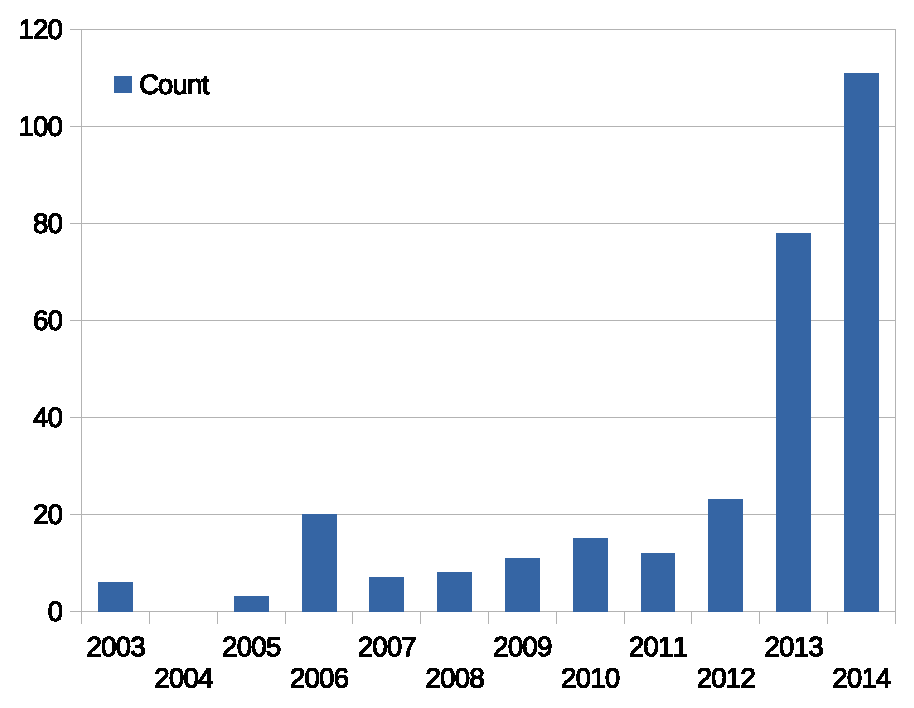
\includegraphics[width=0.6\linewidth]{fig/cubesats_launched_from_2003_to_2014}
\caption{CubeSats launched from 2003 to 2014. Compiled using data from M. Swartwout.}
\label{fig:CubeSats launched from 2003 to 2014}
\end{figure}

\begin{figure}[h]
\centering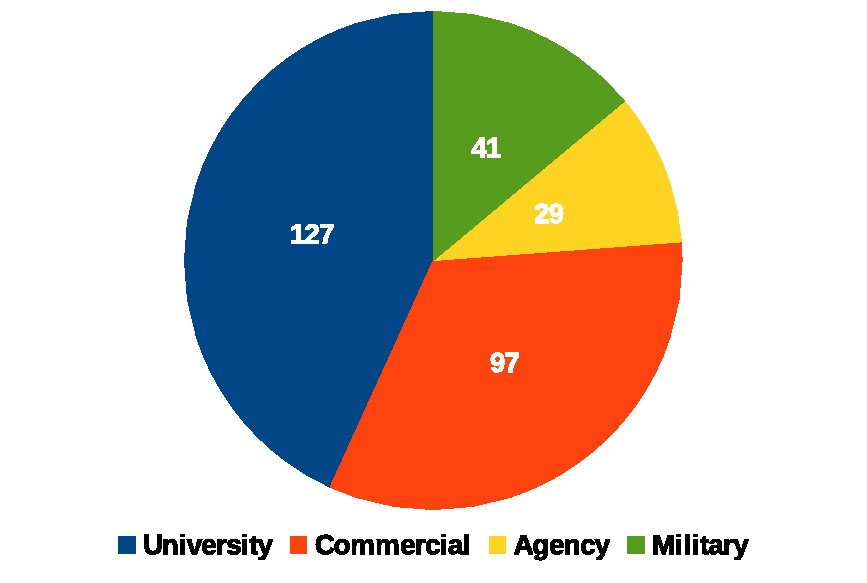
\includegraphics[width=0.8\linewidth]{fig/cubesats_launched_from_2003_to_2014_by_ownership}
\caption{Number of CubeSats that were launched from 2003 to 2014 grouped by ownership. Compiled using data from M. Swartwout.}
\label{fig:CubeSats that were launched from 2003 to 2014 grouped by ownership}
\end{figure}

From this it is evident that academia remains a major player in the CubeSat sector. As such, it has a strong impact on the future of the CubeSat program. CubeSats are an ideal tool for teaching hands-on space technology but they also offer a great chance for opening up the access to space technology to a much larger audience, including students and individuals from developing countries \cite{scholz2015toward}. 

\begin{comment}

\section{Open Source}

The current trend of increasing closed-source commercialization is counter-productive to the objective of opening the access to space. One side effect is that a number of universities have established ``centers of excellence'' for CubeSats, which capitalize on their in-house acquired knowledge. At the same time inter-university collaborations are minimal or not pursued at all. This is arguably not in the original interest of the CubeSat concept, which stipulates the free exchange of design information and lessons learned. 

Terrestrial open source software (OSS) is the backbone of modern society. It is present in almost every field of information technology, such as web servers, operating systems, software development tools, and mobile phones. Open source hardware (OSHW), as discussed in this context\footnote{Radio amateurs, hobbyists, and DIY communities have exchanged design information ever since; here we focus on projects that are made available to a wider public, mainly via the internet.}, is a relatively new phenomenon that follows the same principles: to allow anyone access to its sources for modification, sharing, building, and selling. 

\subsection{Definition}

The combination of open source software and open source hardware is referred to as \textbf{open design}. The recognized authorities for open source software regulation are the Free Software Foundation (FSF) and the Open Source Initiative (OSI), founded in 1985 and 1998, respectively. Both differ to some extent in their goals and values, but from a practical point of view agree on many aspects of what it means to produce free or open software. As a summary of the ten rules for open source definition, the OSI states \cite{opensource.org},

\textit{Open source software is software that can be freely used, changed, and shared (in modified or unmodified form) by anyone. Open source software is made by many people, and distributed under licenses that comply with the Open Source Definition.}

The definition of open source hardware is more complex. This stems from the fact that usage of hardware differs much from software and, being a relatively new phenomenon, less literature on that topic is available. See Lock \cite{lock2013open} for a thorough discussion on this subject. Also, software is easily copied and redistributed, which is not the case for hardware. Hardware modification and production requires access to drawings, schematics, diagrams, design rules, layouts, and other documents.  The Open Source Hardware Association (OSHWA) provides the following definition \cite{oshwa.org}:

\textit{Open source hardware is hardware whose design is made publicly available so that anyone can study, modify, distribute, make, and sell the design or hardware based on that design. The hardware's source, the design from which it is made, is available in the preferred format for making modifications to it.}

Broadly speaking, open source hardware is a physical artifact whose design information is made available under one of the legally binding recognized open source licenses.

\subsection{Intellectual Property Rights}

A number of mechanics are in place to protect the intellectual property of individuals and entities. The most relevant ones for open source design are discussed in the following.

\textbf{Copyright} grants the creator of original work the right to use and distribute it, and to define the conditions therefore. It is a legal concept that is protected well in most countries, and is usually in effect for a certain time, such as the lifetime of the author plus several decades. It applies to published and unpublished works. Main intention is to allow the author to benefit from their work, financially or else. Copyright is a very useful concept as it allows the author to decide on what to do with the work, such as to transfer it into the public domain.

Whereas copyright protects how information is presented, \textbf{patents} cover the subject matter of this information. For example, copyright law may restrict one from making copies of design files for a certain product, but it would not prevent one from making and using that product. Put differently, copyright only governs the expression of the idea, but not the idea itself. This is where patents come into play, which offer the right to exclude others from doing so. In short, patents ensure that the patent owner can take full ownership of its invention with the exclusion of others. Obviously, this is exactly the contrary of what open source design stands for.

\textbf{Trademarks} are typically names, slogans, or symbols, used for identification with goods or services. Trademark rights prevent others from using the same sign for their goods or services, but not from making or offering similar goods or services. As such, they provide a way to label offerings to make them recognizable and accredited by users \cite{anderson2010passport}.

\subsection{Open Source Licenses}

Creators of original work may either write license conditions on their own or adapt or modify existing licenses. Making use of existing licenses provides the advantage of a solid legal groundwork, and they are usually well understood and respected in the community. Basically, an open license is an agreement by the author(s) of original work to allow other people to make use of this work in accordance with the license regulations, without the need of paying licenses fees, as long as the terms of the license are followed. It grants rights to the product, that would otherwise be restricted through copyright or patent law.

Two main categories of open source copyright licenses exist: \textbf{strong copyleft} licenses that require that derivative work must be licensed under the same license; and \textbf{weak copyleft} (i.e. permissive) licenses, which permits the use of different license terms for derived works. The latter would allow modifiers to incorporate their open designs into closed proprietary designs or for merging them with projects which have adopted a different form of open license \cite{katz2012towards}.

Licenses for hardware and software differ naturally \cite{ackerman2008toward}. For software projects, the license ensures that the source code is made available. Hardware licenses on the other hand have to provide terms for the user rights on the design information as well as on the manufacturing and usage of the products. Various licenses are available for hardware and software projects and some of the major ones are briefly introduced in the following. See also \cite{webbink2010packaging} for an exhaustive treatment of open source licenses.

The \textbf{GNU General Public License (GPL)} and the \textbf{GNU Lesser General Public License (LGPL)} are published by the Free Software Foundation \cite{fsf.org}. The GPL allows the user to use, study, share, and modify the received software. It demands that these license conditions are also followed for copies of the original work or derived works. This constitutes a strong copyleft. The LGPL in contrast is a permissive free software license, similar to BSD license and MIT license, that allows developers and companies to use and integrate such work into their own (proprietary) software, without being required to apply the license conditions to their own work. The dominant usage of the LGPL is for software libraries.  

The \textbf{GNU Free Document License (FDL)} was designed for manuals, books, documentations, and other reference material, usually distributed together with open source hardware/software. Similar to the GPL, the FDL gives readers the rights to copy, distribute, and modify, requiring that all derivatives be licensed under the same terms (strong copyleft). A dedicated feature is that when copies are sold in larger quantities, the original document or source must be made available to the reader as well.

\textbf{Creative Commons (CC)} is a non-profit organization that has released several licenses \cite{creativecommons.org}. The creators of original work can easily choose a desired license ``a-la-carte'' that fits their needs in terms of which rights to be waived for others to make use of the work. CC licenses are used for all types of work that underlies copyright, including: books, plays, films, music, photographs, and websites. CC itself does not recommend the use of their licenses for software, although this has been done by some, such as for the Arduino boards.

The Tucson Amateur Packet Radio (TAPR) is an international amateur radio organization that published the \textbf{TAPR Open Hardware License (OHL)} in the flavor of a share-alike license that developers can apply to documentation and schematics \cite{tapr.org}. The key features of the license are that it firstly prevents the filing of patent infringements among people making use of OHL-licensed product, and secondly, that it requires modifiers to include both ``before'' and ``after'' versions of all files that were modified. The license is written in the form of a contract between author and recipient, and constitutes a strong copyleft.

The European Organization for Nuclear Research (Conseil europ\'{e}en pour la recherche nucl\'{e}aire, CERN) has issued the \textbf{CERN Open Hardware License (CERN OHL)} that, similar to what GPL is to software, defines the conditions to the use, copying, modification and distribution of hardware design documentation, and the manufacturing and distribution of products \cite{ayass2012cern}. As with other strong copyleft licenses, any modifications must be licensed under the same license conditions, in order to ensure that the whole community will continue benefiting from improvements.

\end{comment}

\section{Space Standards}

It is common practice to develop spacecraft based on unique designs which are specified and implemented on a project-by-project basis. Any reuse of these system design is usually a by-product of reuse of the whole spacecraft bus. While individual CubeSat developers may have established limited in-house standards or bespoken standards with vendors, these are generally closed and would require significant adaptation across other CubeSat missions.

Similarly, there exists little interface standardization for CubeSats which can be used by individual equipment and instrument developers. While it is true that there are a limited number of physical interfaces applicable for practical use in the space environment, the services and access to these interfaces vary considerably between implementations.

Within the CubeSat developer community there have so far been very few significant attempts to further standardize CubeSat missions. Apart from the CubeSat design specification \cite{cubesat_design_specification}, there exist only a few de-facto standards or best practices. Typically, the solutions that have been developed for CubeSat missions by individual developers are tied very much to the peculiarities of their CubeSat payload and mission objective, with little effort to create sustainable and reusable system components.

The result is that a multitude of CubeSat design solutions are in place, with each mission either inheriting past solutions or developing new ones. However, an increase in the number and complexity of missions and the cost of developing state-of-the-art high-speed data interfaces should trigger a re-thinking within the CubeSat community, towards application of a more standardized approach.

Standardization is an important tool to reduce risks, cost and improve both quality and communication between parties during the preparation and execution of space missions. This is true for any spacecraft mission, and CubeSats are no exception to it.

\subsubsection{Organizations}

A number of organizations exist that are concerned with the development of international standards applicable for space projects. As those standards are often based on vast experience from experts in the field, including lessons learned from past missions, they provide a valuable for meaningful standardization of almost any aspect of typical space missions. For most of these standards the particularities of the spacecraft are not important and hence can be applied to large satellite or CubeSats alike.

This book is concerned with the mapping of available international space standards to the various aspects of developing and running a CubeSat mission. The selection criteria for standards organizations were based on the following:

\begin{itemize}
\item Open: Standards shall be openly available to anyone, preferable through the internet.
\item Free: Standards shall be free of charge and fees.
\item International: Standards shall be available in English and address not national interests but an international audience.
\item Up-to-date: Standards shall be implementable with state-of-the-art components.
\end{itemize}

The organizations found to comply well with these criteria are introduced briefly in the following sections.

The \textbf{Consultative Committee for Space Data Systems (CCSDS)} \cite{ccsds.org} was founded in 1982 for governmental and quasi-governmental space agencies to discuss and develop standards for space data and information systems. Currently composed of "eleven member agencies, twenty-eight observer agencies, and over 140 industrial associates," the CCSDS works to support collaboration and interoperability between member agencies through the establishment of data and system standards. The activities of the CCSDS are organized around six topic areas (see Figure \ref{fig:CCSDS Topic Areas}) and composed of many working groups.

The \textbf{European Cooperation for Space Standardization (ECSS)} \cite{ecss.nl} was initiated to harmonize the requirements from existing standards for space projects, and to provide a single, coherent set of standards for use in (but not limited to) all European space systems development and operation.

The goal of ECSS is to develop a common set of consistent standards for hardware, software, information and activities to be applied in space projects, so that life cycle cost are minimized, while continually improving the quality, functional integrity, reliability and compatibility of all elements of the project. It covers the disciplines shown in Figure \ref{fig:ECSS Disciplines}. 

\begin{figure}[h]
\centering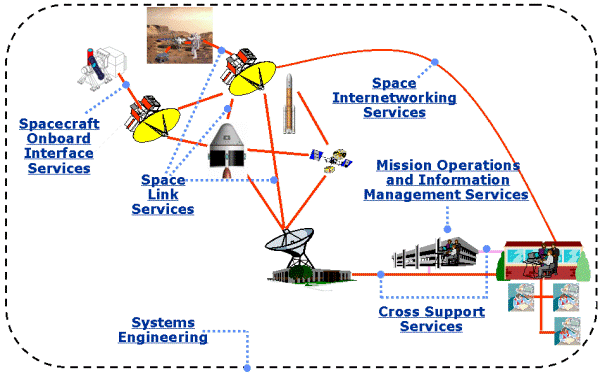
\includegraphics[scale=0.6]{fig/ccsds_topic_areas}
\caption{CCSDS Topic Areas}
\label{fig:CCSDS Topic Areas}
\end{figure}

\begin{figure}[h]
\centering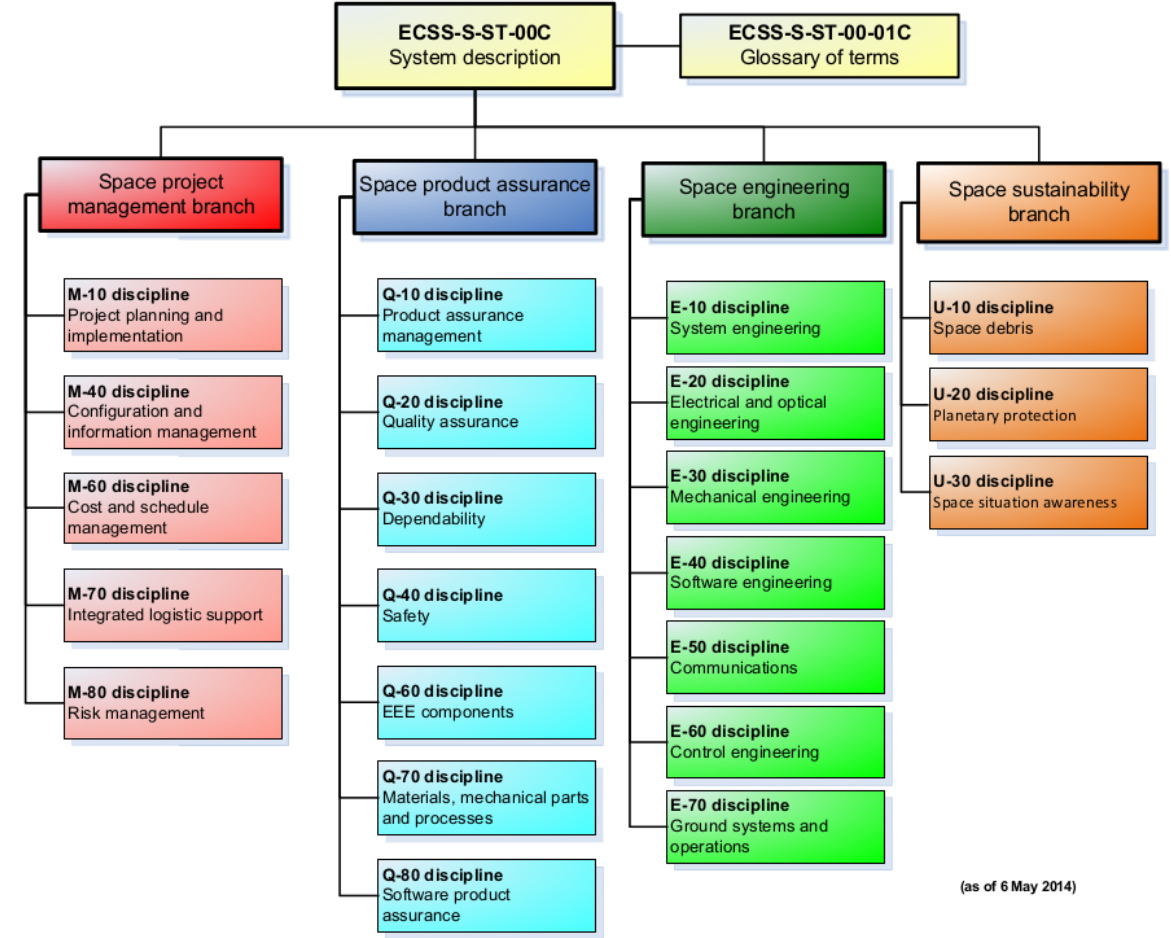
\includegraphics[scale=0.38]{fig/ecss_disciplines}
\caption{ECSS Disciplines}
\label{fig:ECSS Disciplines}
\end{figure}

The \textbf{Object Management Group (OMG)} \cite{omg.org} is an international, open membership, not-for-profit technology standards consortium. OMG Task Forces develop enterprise integration standards for a wide range of technologies and industries. including space industry. OMG modeling standards enable visual design, execution and maintenance of software and other processes. 

The \textbf{Organization for the Advancement of Structured Information Standards (OASIS)} \cite{oasis.org} is a global non-profit consortium that works on the development, convergence, and adoption of standards for security, energy, content technologies, emergency management, and other areas.

\section{How To Use This Book}

This book was written with the goal to improve the overall reliability of CubeSats (in particular from academia and research) and to increase the level of cooperation among CubeSat developers. The application of standards and the mindset of open source software and hardware are the two pillars upon which these goals can be achieved.

This book however does not prescribe in any way what CubeSat developers have to do or which standards shall be required for their project. The book is only a review of existing space standards (mostly from ECSS and CCSDS) and their potential application within CubeSat projects. It is be up to the CubeSat developer team (or the top level customer) to decide which of those standards are selected as binding.

Nonetheless, the recommended approach for CubeSat developers is to follow the development process in a way that is similar to the one outlined in the first part of the book, and to produce \textbf{all} documents listed as deliverables in Section \ref{sec:Project Management Deliverables}, Section \ref{sec:Product Assurance Deliverables}, Section \ref{sec:Engineering Deliverables}, and Section \ref{sec:Mission Operations Deliverables}. Although this may appear as an overwhelming task at first that requires a lot of paperwork, it lays in fact the foundation of a project. It is up to the project team to decide how much effort they put into each of these documents, but it will give a guiding structure to all project related activities and for all the people involved. Last but not least, following this document layout will help in understanding and navigating through other CubeSat projects much quicker.

The second part of the book then presents a large number of standards that are related to system technology and communications protocols. They are categorized into domains of potential application. For example, for onboard communication, the ECSS-CAN bus standard is presented, as it is a standardized space communication bus that is suitable and feasible for implementation in CubeSats. Note however that this part of the book is \textbf{not} a review of technology used on CubeSats or a recipe on how to build a CubeSat. It is rather to show what standards are available that can be possibly used in a CubeSat mission. Most of those standards are concerned with data exchange protocols and interface standardization.

\part{Processes}
\label{part:processes}

\chapterimage{chapter_head_01} % Chapter heading image
\chapter{Project Management}

\section{Overview}

The overall objective of project management is to implement a process to achieve successful completion of the project in terms of \textbf{cost}, \textbf{schedule} and \textbf{technical performance}. Project management is performed following a structured approach throughout all stages of its life cycle and at all levels of the \textbf{customer-supplier chain}.

The notation of customer-supplier model\index{Customer-supplier model} is used throughout this book to denote the concept that  the production of a space system involves parties that supply and parties that consume goods and/or services. In its simplest form, a project can comprise one customer with one or more supplier; however, most space projects comprise a number of hierarchical levels, where:

\begin{itemize}
\item the actor at the top level of the hierarchy is the top level customer (i.e. the stakeholder),
\item the actors at intermediate levels of the hierarchy are both supplier and
customer,
\item the actors at the lowest level of the hierarchy are suppliers only.
\end{itemize}

Project management integrates all management, engineering and product assurance functions required to execute the project.

\subsection{Project Initiation} 

Initially, there is the need or wish to accomplish a certain high level objective for some reason. This could for example be to scan regions of the earth for disaster monitoring. In principle, anybody can propose a space mission. The most common initiators are however: governments, space agencies, science communities, or operators of commercial space systems.

The purpose and objectives of the project are defined by the \textbf{project initiator} in the \textbf{mission statement document} (Section \ref{sec:Mission Statement Document}) which includes key performance parameters and technical and programmatic constraints to be applied to the project. In addition, the overall scope of the project will be defined in terms of the golden triangle: cost, time, and performance.

The \textbf{top-level customer} may or may not be the same as the project initiator. For CubeSat missions, typically the first case is true, where the project initiator takes the role of the top-level customer. The first task of the top-level customer is to prepare a \textbf{project requirements document} (Section \ref{sec:Project Requirements Document}). This is usually done with inputs from (potential) suppliers. The document takes into account the following considerations:

\begin{itemize}

\item \textit{Is there need to develop new technologies?} For most mission some technology has to be developed. However, many parts of a mission can rely on existing, or off-the-shelf, equipment and products. Using available technology not only reduces risk, but you also have to take into account that the development of new technologies is a main driver for project costs and schedule. Therefore make reuse of proven systems wherever feasible. And for those parts that have to be newly developed, assess thoroughly its impact and the required resources.

\item \textit{What are the requirements in terms of human resources?} Although the project team may not have been defined at this stage, the needed skills and approximate number of man hours should be identified. Space projects are interdisciplinary undertakings, requiring skills in management, quality assurance, and engineering. 

\item \textit{What are the requirements on facilities and resources?} A large number of tools and facilities are needed for the design, development, and verification of the system. 

\item \textit{How much risk is acceptable?} Desirably, risks are to be minimized or mitigated. This, however, is a trade-off with costs. 

\item \textit{What development approach to follow?} The approach for the development, that is the number and definition of product models and the associated verification processes, follow from the mission requirements and constraints, but also from the assessment of the above questions. For example, for a low risk mission, a larger number of models are produced, each undergoing intensive verification. This is generally called mission assurance.

\item \textit{What are the deliverables?} The customer has to define all deliverable products needed to meet the mission statement.

\end{itemize}

The \textbf{project requirements document} (PRD) is the integral part of a \textbf{tender}, such as an invitation to tender (ITT), request for proposal (RFP) or request for quote (RFQ). It is released to potential \textbf{top-level suppliers}. Most of requirements are obtained from tailoring the requirements contained in relevant ECSS standards to the specific mission needs. 

\subsection{Project Life Cycle}

Each project is unique and has a distinct life time. The typical life cycle of a space mission covers the following activities:

Objective 
$\rightarrow$ Requirements
$\rightarrow$ Definition
$\rightarrow$ Verification
$\rightarrow$ Production
$\rightarrow$ Utilization
$\rightarrow$ Disposal

\subsection{Project Management Process}

The project management process is implemented by the top-level supplier (and possibly other lower level suppliers in the customer-supplier chain).

Input: 
\begin{itemize}
\item Business agreement / project requirements document
\item Lessons learned from previous projects
\item Applicable standards
\item External information
\item Resources 
\end{itemize}

Process:
\begin{itemize}
\item Project initiation
\item Project planning
\item Project execution
\item Project control and validation
\item Project close-out
\end{itemize}

Outputs:
\begin{itemize}
\item Project products delivered
\item Project objectives achieved 
\item Lessons learned documented
\end{itemize}

\section{Project Management Disciplines}

In order to implement the project management process, a number of disciplines are involved. They are described in the following sections.

\subsection{Planning and Implementation}

\begin{tabular}{l}
\textit{ECSS-M-ST-10 "Project planning and implementation" \cite{ECSS-M-ST-10}}
\end{tabular}

Project planning and implementation is the core of project management. Planning is the process of determining \emph{what has to be done} to achieve the mission objectives and implementation is the process of ensuring that these tasks \emph{are being carried out}, via monitoring and control.

\subsubsection{Project Planning}

The project planning starts immediately after project initiation. Although the top-level customer is responsible for preparing the project requirements document, the top-level supplier is usually already involved at this stage to provide some input.

The \textbf{top-level supplier} responds to the invitation to tender issued by the top-level customer in the form of a \textbf{project management plan} (Section \ref{sec:Project Management Plan}). The project management plan defines the project management approach and methodology to be used throughout the life cycle of the project, together with an overview of all elements of project management disciplines. It includes the definition of the system engineering and product assurance management approach or provides references to separate system engineering and product assurance plans which together make up the total planning documentation used to implement a project.

The project management plan requires input from system engineering and product assurance disciplines and is to be kept up-to-date throughout the entire project life cycle. It remains the key element of project planning. The initial project management plan and any future modifications have to be submitted to the customer for approval.

\subsubsection{Project Organization}

The key for ensuring project success is with project organization. The project organization can be composed of a number of self-standing project teams at the various levels of the customer-supplier chain. More commonly, though, there is a core project team that executes all key functions and makes use of external resources where needed. 

Above all, consistency and coherence are important. Members moving in and out of the team will inevitable cause delay in the project. Yet such situations are unavoidable, in particular in an academic environment. Helpful in such cases is to have a clear definition of the responsibilities of each person (primarily through the means of work packages). 

One of the first actions for the project organization must go into the appointment of the \textbf{project manager}. The project manager is the single person that carries full authority over the project management functions and is the person in charge for contractual matters (such as agreement signing). The project manager also has the task to regularly report to the customer. Although the project manager has the final word, decisions are made in consensus with a steering panel, formed by several project team members of key functions. 

The next step is to appoint the \textbf{key persons} for the each function of the project and access the qualification of the key personal for their tasks, such as system engineering lead or communications system chief engineer. Sometimes a key person takes over more than one key responsibility.

Independent from the allocation of the key persons and their responsibilities it remains with the project management organization (that is, the project manager and the project management team), to do active monitoring and control of all of their own activities and those from all others of the project organization. 

\subsubsection{Breakdown Structures}

Breakdown structures are used to illustrate the composition of complex systems in order to create a common understanding among all actors and to facilitate the project planning process. The different kinds of breakdown structures used in project planning are discussed in the following.

\textbf{Function Tree}\index{Function tree}: The objective of a space mission is implemented via functions. For example, an earth observation mission implements the function of monitoring the earth. Such top level functions are then further decomposed into simpler functions that together perform the higher level tasks. In the current example, the function of monitoring may be decomposed in to image taking, image storage, and image processing. The function breakdown structure is established at the begin of the project and is independent of the products to be used, but it is a vital input to the establishment of the product tree. 

\textbf{Specification Tree}\index{Specification tree}: Whereas functions describe the functionality that shall be achieved, specifications are the means to make those implementations measurable. While the function tree shows \textit{what} the system must achieve, technical specifications define \textit{how} these functions are achieved with certain elements of a system, and specify quantitative and qualitative measures. The specification tree is a graphical representation of all the technical requirements specifications for the different elements of the space system.  The specification tree is based on the technical requirements specification and provides the means to trace back technical requirements to the next higher level of origin. 

\textbf{Product Tree}: The product tree is the breakdown of the space system into successive levels of hardware and software products. It is established at start of Phase B and finalized at end of Phase B. The products in the product tree are chosen as to achieve all the functions specified in the function tree, with the performance level that are specified in the applicable technical requirements specifications. The product tree forms the basis for the project work breakdown structure. Each product tree item shall be attributed with a unique identifier code, an item name, the item supplier, and applicable specification. An example of a product tree is given in Figure \ref{fig:Example of Product Tree}. 

\begin{figure}[h]
\centering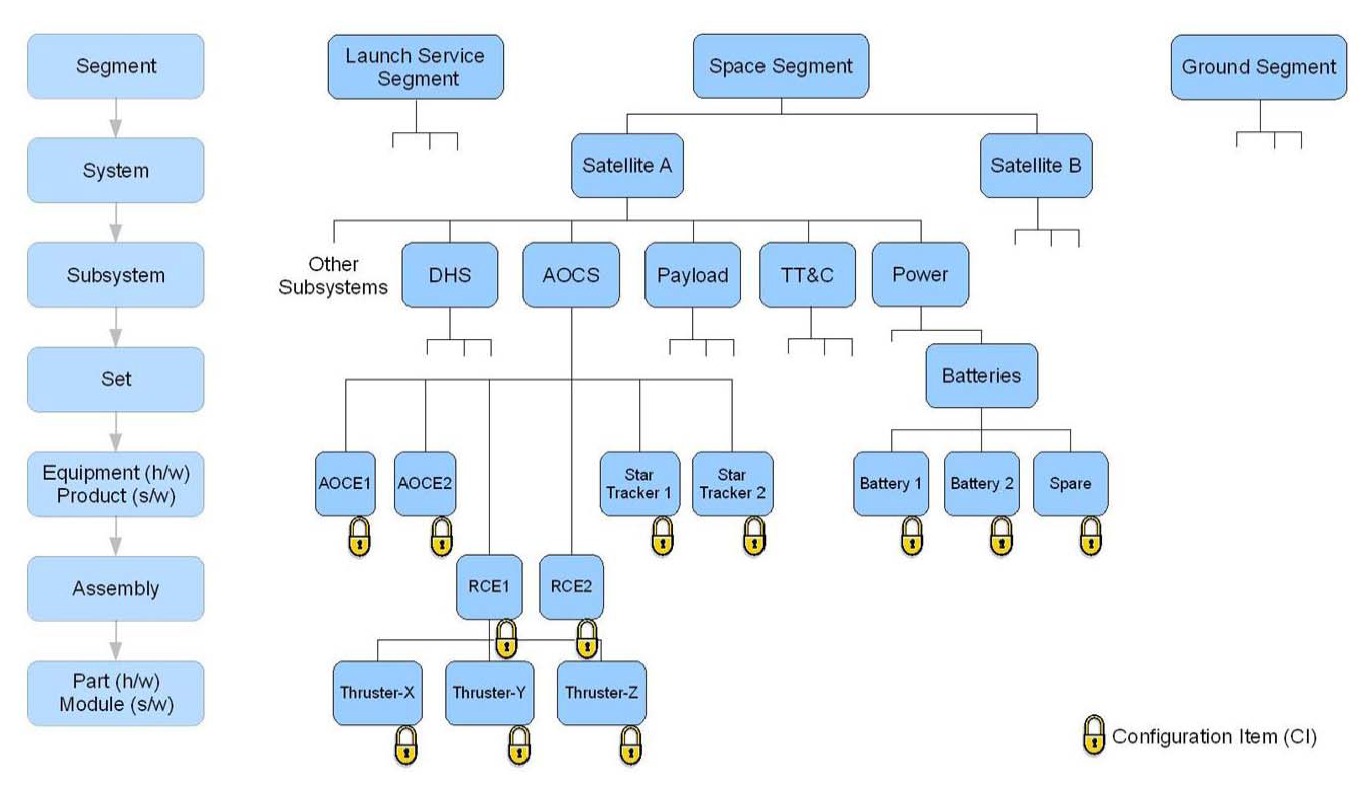
\includegraphics[scale=0.3]{fig/example_of_product_tree}
\caption{Example of Product Tree (ECSS)}
\label{fig:Example of Product Tree}
\end{figure}

\textbf{Work Breakdown Structure}: The work breakdown structure (WBS) is the most important structure to the project manager for managing the project in terms of cost, schedule, and technical content. The WBS divides the project into manageable smaller portions, which are expressed as work packages. The WBS has a hierarchical structure and the appropriate level of detail to which the project is broken down shall be defined by the project manager such that the WBS meets the needs of the project and the nature of the work; yet remains compact and not unnecessary complex. The WBS is derived from the product tree, but also takes into account supporting functions (such as the project management itself, testing activities, productions, etc.) that are necessary to carry out the project. An example of a WBS is provided in Figure \ref{fig:Example of Work Breakdown Structure}. Work related to manufacturing, assembly, integration and test of all product models shall be shown in the WBS.

\begin{figure}[h]
\centering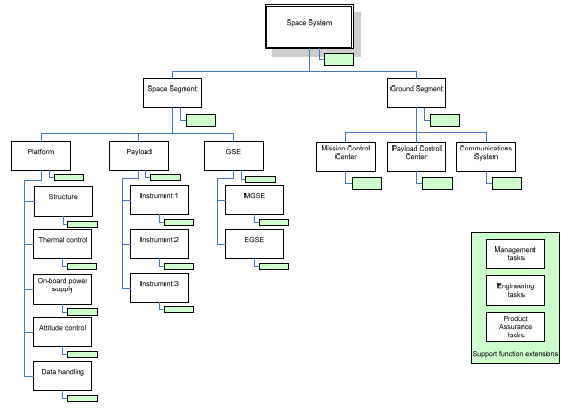
\includegraphics[scale=1.0]{fig/example_of_work_breakdown_structure}
\caption{Example of Work Breakdown Structure (ECSS)}
\label{fig:Example of Work Breakdown Structure}
\end{figure}

Each element in the WBS comprises a certain amount of work, requiring input and producing output. For each element in the WBS a work package description (WPD) shall be established (Section \ref{sec:Work Package Description}). A WP has to have clear definitions on its inputs, it required outputs, the tasks and approach of achieve the outputs, and other details. The purpose of a WPD on lower levels is particularly to separate the higher level complexity from it, such as to let the responsible person concentrate solely on the content of the WPD. A work package may be carried out by a team of people but only a single person is appointed as the responsible WPD manager.

\textbf{Organization Breakdown Structure}: The organization breakdown structure (OBS) depicts the project organization and also shows the contractual interfaces within the organization and to external parties. It shows the hierarchical structure of the key persons and all work package managers.

\subsubsection{Project Phases}

The life cycle of a space project is typically divided into distinct phases. Each phases contains activities to be carried out in the frame of this phase; however, some activities span over several phases. The phasing of a project follows the waterfall model: each phase follows its previous phase. The whole project in turn applies the "V model": From a top level description of the system, and subsequent derivation of requirements, down to its detailed definition; then going up again through verification of lower level then system level, and finally to its operation.

\begin{figure}[h]
\centering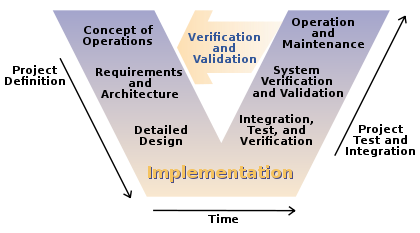
\includegraphics[scale=0.8]{fig/v_model}
\caption{V Model}
\label{fig:V Model}
\end{figure}

The distinct project phases are presented in the following sections. Reviews are held at the end of each phase (with some during a phase) to judge for the go-ahead to the next phase. See Figure \ref{fig:Project Phases and Reviews}.

\begin{figure}[h]
\centering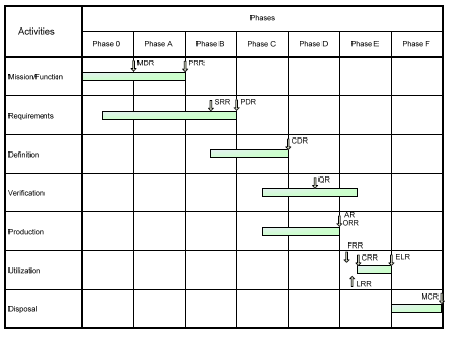
\includegraphics[scale=1.0]{fig/project_phases_and_reviews}
\caption{Project Phases and Reviews (ECSS)}
\label{fig:Project Phases and Reviews}
\end{figure}

\textbf{Phase 0: Mission Analysis and Needs Identification}: This phase is mainly carried out by the project initiator and the top level customer. The major tasks are:
\begin{itemize}
\item Elaborate the mission statement in terms of identification and characterization of the mission needs, expected performance, dependability and safety goals, and mission operating constraints with respect to the physical and operational environment.
\item Develop the preliminary requirements specification.
\item Identify possible mission concepts.
\item Perform preliminary assessment of programmatic aspects.
\item Perform preliminary risk assessment.
\end{itemize}

\textbf{Phase A - Feasibility}: This phase is carried out in order to provide the ground works for the feasibility of the project. The major tasks are:
\begin{itemize}
\item Establish the preliminary PM, SE, and PA plans.
\item Elaborate possible system and operations concepts.
\item Establish the function tree.
\item Assess the technical and programmatic feasibility of the possible concepts.
\item Identify critical technologies and propose pre-development activities.
\item Determine critical elements.
\item Propose the system and operations concept(s) and technical solutions, including model philosophy and verification approach, to be further elaborated during Phase B.
\item Elaborate risk assessment.
\end{itemize}

 It involves the establishment of the preliminary PM, SE, and PA plans, trade-off studies of different system concepts and architectures (including model philosophy and verification approach), the establishment of the function tree, the identification of critical technologies and pre-development activities, and the elaboration of the risk assessment.

\textbf{Phase B - Preliminary Definition}: The major tasks of this phase are:
\begin{itemize}
\item Finalize the PM, SE, and PA plans.
\item Elaborate the baseline master schedule and baseline.
\item Elaborate the preliminary organizational breakdown structure.
\item Select the system and operations concept, as well as the technical solution, and the verification concept.
\item Establish the preliminary design definition for the selected concept.
\item Identify and define external interfaces.
\item Initiate pre-development work on critical technologies.
\item Initiate procurement of long lead items.
\item Finalize product tree, work breakdown structure, and specification tree.
\item Update risk assessment and conduct reliability and safety assessment.
\end{itemize}

\textbf{Phase C - Detailed Definition}: The activities of this phase are driven by the selected model philosophy and verification approach. The major tasks of this phase are:
\begin{itemize}
\item Completion of the detailed design definition of the system down to the lowest level.
\item Production, development testing and pre-qualification of selected critical elements.
\item Production and development testing of engineering models, as required
by the selected model philosophy and verification approach.
\item Completion of assembly, integration and test planning for the entire system.
\item Detailed definition of internal and external interfaces.
\item Issue of preliminary user manual.
\item Update of the risk assessment.
\end{itemize}

\textbf{Phase D - Qualification and Production}: The major tasks of this phase are:
\begin{itemize}
\item Complete manufacturing, assembly and testing of flight hardware/software and associated ground support hardware/software.
\item Complete verification program (qualification and acceptance stages).
\item Prepare system for delivery.
\end{itemize}

\textbf{Phase E - Operations and Utilization}: The activities of this phase depend widely on the type of project and mission. In general, the major tasks of this phase are:
\begin{itemize}
\item Perform all activities at space and ground segment level in order to prepare the launch.
\item Conduct all launch and early orbital operations.
\item Perform on orbit verification (including commissioning) activities.
\item Perform all on orbit operations in order to achieve the mission objectives and perform all ground segment and ground support activities in order to support the mission.
\item Finalize the disposal plan.
\end{itemize}

\textbf{Phase F - Disposal}: The major task of this phase is to implement the disposal plan.

\subsubsection{Reviews}

\begin{tabular}{l}
\textit{ECSS-M-ST-10-01 "Organization and conduct of reviews" \cite{ECSS-M-ST-10-01}} 
\end{tabular}

Reviews are milestones of a project to examine the status and completeness of the project at that point of time against the expected status. Normally, the review board includes external participants that further contribute with their objective view to the critical assessment of the project. Additionally, reviews can identify potential lessons learned.

Reviews are carried out throughout the project life cycle at all levels from mission to unit level. The review purpose, mandate and documentation vary for each particular project and for the specific phase or stage of activity of the project. 

\textbf{Review Bodies}: The participants of a review shall be composed of:
\begin{itemize}
\item The \textbf{review authority / review board}: Appointed by the customer, composed of members of customer organization and external participants that provide further objectiveness to the review.
\item The \textbf{review team}: Appointed by review authority, composed of people preferably with no direct involvement in the project. One single person of this team shall be appointed as review team leader.
\item The \textbf{project team}: Composed of all or a representative subset of the supplier team.
\end{itemize}

\textbf{Review Process}: The course of a review consists of the following steps:
\begin{enumerate}
\item The customer appoints the review authority, the review team, and review team leader.
\item The project team prepares the review procedure (Section \ref{sec:Review Procedure}), which is then subject to the customer's approval.
\item The project team supplies the review data packages subject to review to the review team. The project team is further responsible for the practical implementation of the review, including an optional kick-off meeting (for defining the review objectives), intermediate coordination meetings (as needed), and the final meeting involving all review bodies.
\item The review team reviews the documentation, identifies problems and makes recommendations or requests clarifications in the form of review item discrepancies (Section \ref{sec:Review Item Discrepancy}), and prepares a report (Section \ref{sec:Review Team Report}). 
\item After a certain period during which the project team can respond to the review team in order to close review item discrepancies (RIDs), the review authority will take the final disposition about open RIDs and issue its final report (Section \ref{sec:Review Authority Report}).
\end{enumerate}

\textbf{Mission Definition Review (MDR)}: The primary objective of this review is to release the mission statement and assess the preliminary technical requirements specification and programmatic aspects.

\textbf{Preliminary Requirements Review (PRR)}: The primary objectives of this review are:
\begin{itemize}
\item Release of preliminary management, engineering and product assurance plans.
\item Release of the technical requirements specification.
\item Confirmation of the technical and programmatic feasibility of the system concept(s).
\item Selection of system and operations concept(s) and technical solutions, including model philosophy and verification approach, to be carried forward into Phase B.
\end{itemize}

\textbf{System Requirements Review (SRR)}: This review is held during the course of Phase B. The primary objectives of this review are:
\begin{itemize}
\item Release of updated technical requirements specifications.
\item Assessment of the preliminary design definition.
\item Assessment of the preliminary verification program.
\end{itemize}

\textbf{Preliminary Design Review (PDR)}: The primary objectives of this review are:
\begin{itemize}
\item Verification of the preliminary design of the selected concept and technical solutions against project and system requirements.
\item Release of final management, engineering and product assurance plans.
\item Release of product tree, work breakdown structure and specification tree.
\item Release of the verification plan (including model philosophy).
\end{itemize}

\textbf{Critical Design Review (CDR)}: The primary objectives of this review are:
\begin{itemize}
\item Confirm compatibility with external interfaces.
\item Release the final design.
\item Release assembly, integration and test planning.
\item Release flight hardware/software manufacturing, assembly and testing.
\item Release of user manual.
\end{itemize}

\textbf{Qualification Review (QR)}: The primary objectives of this review are:
\begin{itemize}
\item Confirm that the verification process has demonstrated that the design, including margins, meets the applicable requirements.
\item Verify that the verification record is complete at all levels of the system.
\item Verify the acceptability of all waivers and deviations. 
\end{itemize}

\textbf{Acceptance Review (AR)}: The primary objectives of this review are:
\begin{itemize}
\item Confirm that the verification process has demonstrated that the product is free of workmanship errors and is ready for subsequent operational use.
\item Verify that the acceptance verification record is complete at all levels of the system.
\item Verify that all deliverable products are available per the approved deliverable items list.
\item Verify the "as-built" product and its constituent components against the required "as designed" product and its constituent components.
\item Verify the acceptability of all waivers and deviations.
\item Verify that the Acceptance Data Package is complete.
\item Authorize delivery of the product.
\item Release the certificate of acceptance.
\end{itemize}

\textbf{Operational Readiness Review (ORR)}: The primary objectives of this review are:
\begin{itemize}
\item Verify readiness of the operational procedures and their compatibility with the flight system.
\item Verify readiness of the operations teams.
\item Accept and release the ground segment for operations.
\end{itemize}

\textbf{Flight Readiness Review (FRR)}: The flight readiness review is conducted prior to launch. The objective of this review is to verify that the flight and ground segments including all supporting systems such as tracking systems, communication systems and safety systems are ready for launch.

\textbf{Launch Readiness Review (LRR)}: The launch readiness review is conducted just prior to launch. The objective of this review is to declare readiness for launch of the launch vehicle, the space and ground segments including all supporting systems such as tracking systems, communication systems and safety systems and to provide the authorization to proceed for launch.

\textbf{Commissioning Result Review (CRR)}: The commissioning result review is held at the end of the commissioning as part of the in-orbit stage verification. It allows declaring readiness for routine operations/utilization. This Review is conducted following completion of a series of on-orbit tests designed to verify that all elements of the system are performing within the specified performance parameters. Successful completion of this review is typically used to mark the formal handover of the system to the project initiator or to the system operator.

\textbf{End of Life Review (ELR)}: This review is conducted to verify that the mission has completed its useful operation or service and to ensure that all on-orbit elements are configured to allow safe disposal.

\textbf{Mission Close-Out Review (MCR)}: This review is conducted to ensure that all mission disposal activities are adequately completed.

\subsection{Configuration Management}
\label{sec:Configuration Management}

\begin{tabular}{l}
\textit{ECSS-M-ST-40 "Configuration and information management" \cite{ECSS-M-ST-40}}
\end{tabular}

Configuration management (CM) is the process for establishing and maintaining a consistent record of a system's functional and physical characteristics ("as built") compared to its design and operational requirements ("as designed"). Configuration management is applied throughout the entire life cycle of the product and allows to know at any time the technical description of a product using approved documentation. It helps to record, control, and provide traceability of the evolution in the technical description of a system and ensures the consistency of internal interfaces. It further allows to verify and demonstrate to all actors that documentation is and remains the exact image of the products it describes.

Configuration management interfaces with engineering, product assurance, manufacturing and production, and operations. The supplier produces the \textbf{configuration management plan} (Section \ref{sec:Configuration Management Plan}). The four main tasks of CM are described in the following sections.

\subsubsection{Configuration Identification}

The product tree is used for the selection of \textbf{configuration items} (CIs). CIs fall in two categories: developed or non-developed. The latter is for products that are off-the-shelf, or available from previous projects. Configuration items are identified at various levels of the product tree. There are no fixed rules for which item to select as configuration item, but each selected CI is subject to full configuration management. One generally selects those items that are likely subject to configuration change, be it in hardware or software configuration, or items that the configuration management wishes to have control over (such as the baseline of the ground infrastructure). Each CI shall be labelled with a unique identifier, composed of a part identifier and a serial or lot number (for hardware) or version number (for software). The identifier shall be placed on the item itself if possible, or linked to it. The list of all selected configuration items is maintained in the \textbf{configuration item list} (Section \ref{sec:Configuration Item List}).

\subsubsection{Configuration Control}

During the life cycle of the project several configuration baselines are defined and agreed upon. Configuration control is the process for controlling the evolution of those baselines.

Changes to configuration items can only be done through change control procedures. Changes on \textbf{requirements} are done through \textbf{change requests} or \textbf{change proposals}. Change requests (Section \ref{sec:Change Request}) come from the customer (e.g. for evolution of requirements), whereby change proposals (Section \ref{sec:Change Proposal}) come from the supplier (e.g. self initiated improvement of design). The \textbf{configuration control board}, which can be a single person or a team appointed by the project manager, takes decision on those requests; and in case of major departures from the baseline it does this in coordination with the customer.

Before production, the supplier may request changes to the \textbf{configuration items} through \textbf{requests for deviation}. A request for deviation (Section \ref{sec:Request for Deviation}) is used to agree on the planned departure from the customers requirement that is part of an approved configuration baseline. After production, when the supplier discovers non-conformance of configuration items, a \textbf{requests for waiver} may be applied.  A request for waiver (Section \ref{sec:Request for Waiver}) is used to agree on the use and/or delivery of a product that is not conform to the approved product configuration baseline.

For changes during the operational phase of the mission the same principle apply.

\subsubsection{Configuration Status Accounting}

Configuration status accounting provides the ability to record and report on the configuration baselines at any moment of time. An important tool for this is the \textbf{configuration item data list} (Section \ref{sec:Configuration Item Data List}) that lists all relevant technical documents and their version number for each configuration item (including references to lower level configuration items). The \textbf{as-built configuration data list} (Section \ref{sec:As-Built Configuration Data List}) is a document to act as reporting instrument defining the physical as-built status of each configuration item and listing any discrepancies to the configuration item data list (CIDL). The \textbf{software configuration file} (Section \ref{sec:Software Configuration File}) is used for reviews, and created for each configuration item that involves software development.

\subsubsection{Configuration Verification}

The project reviews (and possibly occasional audits) are used for verification of the configuration.

\subsection{Information Management}

\begin{tabular}{l}
\textit{ECSS-M-ST-40 "Configuration and information management" \cite{ECSS-M-ST-40}}
\end{tabular}

Information management is concerned with the life cycle of documents, that is the creation, collection, review, delivery, storage, archiving, and retrieval of them. All documents are managed electronically.

\subsubsection{Document Reference Number}

Each newly created document is assigned a unique reference number. The structure of such reference number is mission specific and may, for example, be structured as

\texttt{<ORG>-<Project>-<WBS\#>-<Type>-<Number>}. 

For the first "minutes of meeting" document regarding the element "5500" in the work breakdown structure of  project "CSAT" from organization "CORG" this yields the reference number 

\texttt{CORG-CSAT-5500-MIN-0001}. 

A list of ISO conform identifiers for element "Type" is given in Section \ref{sec:Common Document Types}.

\subsubsection{Document Status}

When a new document is created and assigned a reference number, it bears the status "in preparation". It is considered preliminary and cannot be used for binding agreements. When it is complete, it will be submitted for review and bears the status "under review". As the outcome of the review the documents status may change to "rejected" (if it did not pass the review), "superseded" (if it was replaced by another document), or "approved". The document is then digitally signed.

\subsubsection{Document Version}

Once approved the document is valid for use and for binding agreements. Any modification to the document implies a new version. The version of a document is updated in the document  and the document file is appended by its issue number and revision number in the form \_iXrY, where X is the issue and Y is the revision. Before the approval of a document its issue number is zero (0) and the revision number shall start with a one (1) and be incremented upwards. The first approved issue of a document is \_i1r0. Minor changes affect the revision whereas major changes (such as design reviews) change the issue. For the above example, the second issue and first revision of the document would yield the complete reference as 

\texttt{CORG-CSAT-5500-MIN-0001\_i2r1}.

Every change of a document shall be approved and digitally signed to take affect.

\subsubsection{File Formats}

File formats for electronic documents are preferably open formats. Some examples are:

\begin{itemize}
\item PDF for signed read only documents
\item OpenDocument formats for editable text documents, spreadsheets, presentations
\item JPEG for photographic images
\item PNG or TIFF for technical images
\item SVG for vector graphics
\item ZIP for packed archives
\end{itemize}

For other types of data (such as CAD drawings, PCB layout, circuit schematics) open exchange formats are preferred where available.

\subsubsection{File Exchange}

File exchange is preferably done using ZIP files as container.

\subsubsection{Document Management System}

The document management system shall ensure that project information/documentation is

\begin{itemize}
\item preserved from damage or loss,
\item accessible and retrievable,
\item access controlled to authorized users.
\end{itemize}

\subsection{Cost Management}

\begin{tabular}{l}
\textit{ECSS-M-ST-60 "Cost and schedule management" \cite{ECSS-M-ST-60} }
\end{tabular}

Cost management includes the activities to complete the project with a defined budget, namely through cost estimation and planning, cost control, and cost reporting. It facilitates the predication of potential budget deviations and the implementation of countermeasures to avoid cost overruns. Cost management is strongly tied to schedule management. Cost management may establish a business agreement structure diagram to identify the cost reporting relationships between respective customers and suppliers. A useful tool for supporting cost management is the cost breakdown structure (Annex A of ECSS-M-ST-60 provides details).

\subsubsection{Cost Estimating and Planning}

Cost estimating is the process of determining the expected costs of a project. Different methods for cost estimation can be applied. Commonly, a top-down approach (i.e. referring to cost data from similar projects) is used at early phases of the project and bottom-up approaches (i.e. analyzing each individual work package and summing it all up) at later phases. In particular for the bottom-up approach, the work breakdown structure of the project is an important input. This transforms the work breakdown structure into a cost breakdown structure. Cost estimations (see Annex E of ECSS-M-ST-60) are supplied to the customer at agreed milestones and to be updated throughout the project.

\subsubsection{Cost Control}

The customer approved cost estimation forms the \textbf{original baseline cost plan}, which is updated continuously as the \textbf{current baseline cost plan}. In order to allow better control over the costs, two key numbers are continuously updated: the estimate at completion (EAC) and the estimate to completion (ETC). The EAC gives an estimate of the total expenses of the project upon its completion, whereas the ETC is the total expenses for work to be performed from now until the work is completed.

\subsubsection{Cost Reporting}

Depending on the agreement, the supplier periodically submits reports about the cost evolution to the customer. These are namely the original and current baseline cost plan, and the EAC and ETC numbers.

\subsection{Schedule Management}

\begin{tabular}{l}
\textit{ECSS-M-ST-60 "Cost and schedule management" \cite{ECSS-M-ST-60}}
\end{tabular}

Schedule management includes the activities to complete a project within a defined time, namely through establishment of the schedule, schedule control, and schedule reporting. 

\subsubsection{Schedule Definition}

Scheduling takes into account the work to be performed versus the available resources to implement this work and produces a schedule down to sufficient detail. A schedule is actually a network of activities and milestones, together with the relationships between them (see Annex B of ECSS-M-ST-60 for details). For instance, some activities may run in parallel but some activities may depend on the completion of other activities before they can start. 

The work breakdown structure is the input to the schedule definition. The activities are put in sequence and linked to each other reflecting the logical dependencies between them. Next, the duration is estimated for each activity and the required resources. This is then translated into a schedule using a working calendar as basis, that specifies the working hours, holidays, and so on. 

There are also a number of milestones to be placed in the schedule. Traditionally they serve as "gates", which need to be passed in order to proceed with following activities. At minimum, the following milestones are defined: start/end of project, reviews, delivery dates, and business agreement milestones. Figure \ref{fig:Example of Gantt Chart} shows an example Gantt chart as outcome of the schedule definition process.

\begin{figure}[h]
\centering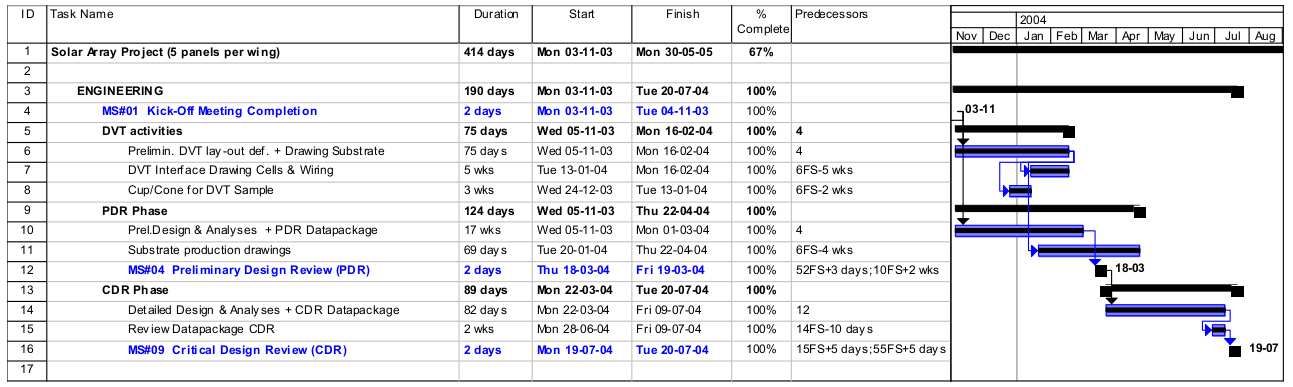
\includegraphics[scale=0.3]{fig/example_of_gantt_chart}
\caption{Example of Gantt Chart (ECSS)}
\label{fig:Example of Gantt Chart}
\end{figure}

\subsection{Schedule Control}

Two schedules are used for schedule control: the baseline schedule and the current working schedule. 

The \textbf{baseline schedule} is the reference schedule that was approved by the customer and allows for timely completion of the project or project phase. It is established through the schedule definition task as already explained. It contains as a minimum the milestones, description and duration of activities, the start and finish dates of activities, and the identification of the critical path. The critical path is the sequence of project network activities which add up to the longest overall duration. This determines the shortest time possible to complete the project.

The \textbf{current working schedule} on the other hand documents the actual status of completed and planned activities, and is updated continuously. It reflects the most realistic view of the project status.

Both schedules are identical at start of the project. As the project progresses, the current working schedule can differ, due to differences in planned and actual progress. This identification of those differences form the basis for progress assessment and the possible implementation of countermeasures to bring the schedule back on track.

\subsubsection{Schedule Reporting}

Schedule reporting is needed to inform the customer about the project progress. The regularity of such reporting is agreed between supplier and customer, and comprise at a minimum details on: activities started/completed, completion forecast for ongoing activities, and an assessment of the logical between activity relationships (see Annex C of ECSS-M-ST-60 for details).

Such progress updates may be conveyed during progress meetings, progress reports, and reviews. Independent from such regular progress updates, if there are major delays in the schedule then the customer shall be informed immediately.

\subsection{Integrated Logistic Support}

\begin{tabular}{l}
\textit{ECSS-M-70 "Integrated logistic support" \cite{ECSS-M-70}}
\end{tabular}

Integrated logistic support (ILS) is a process for developing material resources and services essential to support development, operation and maintenance. The purpose of it is to maintain the technical and availability performance levels while respecting safety constraints and optimizing overall life cycle cost.

Factors of logistic needs are usually: support facilities and equipment, support tools (including software), personnel skills and training, and maintenance plans.  

Integral part of ILS is also inventory control, namely for EEE parts, consumables, equipment, and custom items.

\subsection{Risk Management}
\label{sec:Risk Management}

\begin{tabular}{l}
\textit{ECSS-M-ST-80 "Risk management" \cite{ECSS-M-ST-80}}
\end{tabular}

Risks impact the cost, schedule, or technical performance of a project and therefore present a danger to project success. The objective of risk management is to identify, assess, reduce, accept, and control risks. Proper risk management allows optimization of the overall cost of a project.

The mitigation of risks already starts with the implementation of a systematic methodology for all space project disciplines, namely project management, product assurance, system engineering, and mission operations. Risk management is to be carried out on a day-to-day basis.

The risk management process includes the establishment of a risk management policy, the identification and assessment of risks, the decision on risks, and risk monitoring. The later three steps are carried out in a continuous loop throughout the project life cycle.

Policy
$\rightarrow$ Identify
$\rightarrow$ Decide
$\rightarrow$ Monitor
$\rightarrow$ Identify
$\rightarrow$ etc.

\subsubsection{Risk Management Policy and Plan}

The \textbf{risk management policy document} (Section \ref{sec:Risk Management Policy Document}) describes the objective and principles of risk management in the context of the project. It specifies on a high level the criteria for classification and acceptance of risks. This includes for example the definition of scoring schemes for risk likelihood and severity, and the risk indexing.

The \textbf{risk management plan} (Section \ref{sec:Risk Management Plan}) on the other hand specifies how risk management is implemented, such as roles and responsibilities of people.

\subsubsection{Risk Identification and Assessment}

Risk identification is to be performed in all disciplines and levels of the project. Risks may be of technical, cost, schedule, or other nature. Each member of the engineering team shall be responsible for continuously assessing the risks on their part of the project through the project life cycle, recording this in the form of a project-level risk register, and communicating the risk assessment to the project manager and system engineer.

Every identified risk scenario should be assessed in terms of its causes and consequences, in accordance with the risk policy. In particular, the risk shall be further quantified in terms of severity, likelihood, and so on, and added to the \textbf{risk assessment report} (Section \ref{sec:Risk Assessment Report}).

\subsubsection{Decision on Risks}
 
Identified risks may be either mitigated or accepted. Usually, risks that have minor impact but are costly to avoid are accepted. Risks however which do have a more severe impact on the project and are unacceptable should be avoided by all means possible. If avoidance is not feasible, then this must be communicated to the customer.

The project manager shall maintain the \textbf{risk register} (Section \ref{sec:Risk Register}) and delegate to the system engineer the responsibility to properly address these risks with the engineering team through the planning of specific activities to mitigate them. The project manager and system engineer shall then assign the responsibility for carrying out the risk mitigation actions to individual members of the project engineering team.
 
\subsubsection{Risk Monitoring}

The project manager shall use the risk register to regularly communicate the project risks and mitigation action plans. Periodically all identified risks shall be re-assessed. Further, the implementation of risk reduction performance shall be reviewed over time. One way to visualize this is the use of a risk trend chart. 
  
\clearpage
\section{Deliverables}
\label{sec:Project Management Deliverables}

\subsection{Documents per Review}
\begin{table}[h]
\centering
\begin{tabular}{l c c c c c c c c c}
\toprule
\textbf{Phase} & \textbf{0} & \textbf{A} & \multicolumn{2}{c}{\textbf{B}} & \textbf{C} & \multicolumn{2}{c}{\textbf{D}} & \multicolumn{2}{c}{\textbf{E}} \\
\textbf{Review} & \textbf{MDR} & \textbf{PRR} & \textbf{SRR} & \textbf{PDR} & \textbf{CDR} & \textbf{QR} & \textbf{AR} & \textbf{ORR} & \textbf{FRR} \\
\midrule
Project management plan         &   & •  & • & • &   &   &   &   &   \\
\hline
Product tree					&   & • & • & • & • & • & • &   &   \\
\hline
Work breakdown structure 		&   & • & • & • &   &   &   &   &   \\
\hline
Work package description     	&   & • & • & • &   &   &   &   &   \\
\hline
Schedule						& • & • & • & • & • & • & • & • & • \\
\hline
Cost estimate report			&   & • & • & • &   &   &   &   &   \\
\hline
Config. management plan 		&   & • & • & • &   &   &   &   &   \\
\hline
Config. item list				&   &   &   & • & • &   &   &   &   \\
\hline
Config. item data list			&   &   &   & • & • & • & • &   &   \\
\hline
As-built config. list			&   &   &   &   &   & • & • &   &   \\
\hline
Software config. list			&   &   &   & • & • & • & • &   &   \\
\hline
Config. status acc. reports		&   &   &   & • & • & • & • &   &   \\
\hline
Risk management policy doc.	    & • & • & • & • &   &   &   &   &   \\
\hline
Risk management plan			& • & • & • & • &   &   &   &   &   \\
\hline
Risk assessment report			&   & • & • & • & • & • & • & • & • \\
\bottomrule
\end{tabular}
\caption{Management Documents required per Review}
\end{table}

\subsection{Documents per Request}
\begin{itemize}
\item Cost breakdown structure
\item Schedule progress report
\item Cost estimating plan
\item Inventory record
\item Cost and manpower report
\item Risk register
\end{itemize}

\chapterimage{chapter_head_01} % Chapter heading image
\chapter{Product Assurance}

\section{Overview}

The prime objective of product assurance is to ensure that space products accomplish their defined mission objectives in a safe, available and reliable way. In support of project risk management, product assurance assures an adequate identification, appraisal, prevention and control of technical risks within project constraints.

\section{Product Assurance Disciplines}

In order to implement the product assurance process, a number of disciplines are involved. They are described in the following sections.

\subsection{Product Assurance Management}

\begin{tabular}{l}
\textit{ECSS-Q-ST-10 "Product assurance management" \cite{ECSS-Q-ST-10}}
\end{tabular}

Product assurance management is a multidisciplinary activity to ensure that a product assurance program is implemented and managed throughout all project phases and coordinated with all actors. It addresses the \textbf{product assurance plan} (Section \ref{sec:Product Assurance Plan}) defining all product assurance activities consistent with the project objectives, requirements, criticalities and constraints. 

In particular it includes the allocation and availability of adequate resources, personnel and facilities to carry out the necessary tasks and to follow up progress monitoring, reporting and visibility of all product assurance matters, in particular those related to alerts, critical-items, nonconformances, changes, deviations, waivers, actions or recommendations resulting from reviews, inspection and audits, qualification, verification and acceptance.

The product assurance (PA) manager shall ensure that a \textbf{qualification status list} (Section \ref{sec:Qualification Status List}) is maintained throughout the project lifetime.

\subsubsection{Critical-Item Control}
\label{sec:Critical-Item Control}

\begin{tabular}{l}
\textit{ECSS-Q-ST-10-04 "Critical-item control" \cite{ECSS-Q-ST-10-04}}
\end{tabular}

Critical items (CI) are potential threats to the performance, quality, dependability and safety of a system that are controlled by a specific action plan in order to mitigate emanating risks and to prevent undesirable consequences. Such items shall be formally identified and controlled in a \textbf{critical-item list} (Section \ref{sec:Critical-Item List}). 

Various product assurance analysis provide considerable inputs for identification of critical items (e.g. RAMS: FMECA results, hazard analysis results; PMP: non-qualified parts materials and processes; EEE: non-qualified parts or new technology; lessons learned from previous programs). Annex C of ECSS-Q-ST-10-04 provides a guide for identifying critical items.

The control process for critical items is similar to the risk management process and bears interface to it, namely:

\begin{itemize}
\item critical-item inputs to the risk identification activity, 
\item risk classifications used to prioritize critical items, 
\item references between risk reduction and critical item control measures, 
\item status of critical-item control implementation. 
\end{itemize}

In addition to the critical-item list, \textbf{critical-item control forms} (Section \ref{sec:Critical-Item Control Form}) shall be created and maintained by the PA manager.

\subsubsection{Nonconformance Control}
\label{sec:Nonconformance Control}

\begin{tabular}{l}
\textit{ECSS-Q-ST-10-09 "Nonconformance control system" \cite{ECSS-Q-ST-10-09}}
\end{tabular}

Whenever in the project lifetime a nonconformance is detected, the product assurance representative shall analyse and document it in a \textbf{nonconformance report} (Section \ref{sec:Nonconformance Report}). This report is then to be submitted to the internal nonconformance review board (NRB) for assessment, which classifies it as either minor or major, and maintains a list of all identified nonconformance items and their status (Section \ref{sec:NCR Status List}).

Major nonconformances are those that have an impact on safety, reliability, maintainability, lifetime, interchangeability, or on operational, functional, or contractual requirements.

Minor and major nonconformances are disposed in either of the following ways: return to supplier (for procured items), use "as-is", rework, scrap, or repair. The difference between handling of minor and major nonconformances is that minor ones are decided and acted upon within the project team, whereas major ones have to be addressed together with the customer.
 
Although ECSS-Q-ST-10-09 also covers operational nonconformances during mission operations phase, these are better to be handled with dedicated anomaly reports as discussed in Section \ref{sec:Operations Reporting}.

\subsection{Quality Assurance}

\begin{tabular}{l}
\textit{ECSS-Q-ST-20 "Quality assurance" \cite{ECSS-Q-ST-20}}
\end{tabular}

Quality assurance (QA) is the main pillar of product assurance. Quality assurance management focuses on ensuring the quality throughout the design, verification, procurement, manufacturing, assembly, integration, testing, acceptance, and delivery of the product. The \textbf{quality assurance plan} (Section \ref{sec:Quality Assurance Plan}) provides details on all these aspects. 

In addition, a documented training/certification plan shall be established for personnel, whose performance determines or affects product quality, and records of such trainings shall be maintained.

The quality assurance comprises the following phase-independent activities:

\begin{itemize}
\item critical-items control (Template \ref{sec:Critical-Item Control})
\item nonconformance control (Template \ref{sec:Nonconformance Control})
\item alert management 
\item stamp control
\item traceability 
\item metrology and calibration 
\item handling, storage and preservation

\end{itemize}

An \textbf{alert management system} is used to inform the customer on issues that are detected and that do not fall under nonconformance category, with possibly impact on other projects. Typically this is for (generic) software applications or support equipment. An incident management system can be used for this.

\textbf{Stamp control} refers to methods of implementing a correct and legitimate authorizations system, to ensure, for example, that digital signatures are protected and trustful.

\textbf{Traceability} means that there is maintained a relationship between parts, materials, or products and their associated documentation. This is largely covered in Section \ref{sec:Configuration Management}.

Broadly speaking, \textbf{metrology and calibration} refers to proper control, calibration and maintenance of measurement and test equipment. 

For the \textbf{handling, storage and preservation} of items, proper means shall be established to prevent damages during all phases, from manufacturing to operations. ECSS-Q-ST-20-08 \cite{ECSS-Q-ST-20-08} addresses this for spacecraft hardware in detail.

\subsubsection{Design and Verification}

Quality assurance principles for design and verification phase comprise the definition of design rules and methods, the selection of tools, and to ensure that the design is producible and repeatable.

The use of \textbf{space qualified parts} in system design significantly adds to the quality of the system in terms of reliability. The ESCC (European Space Components Coordination) for example publishes a list of components and technologies which have been, respectively, qualified and capability approved by ESA. \cite{spacecomponents.org}

Another aspect of quality assurance covers the use of \textbf{off-the-shelf} (OTS) hardware items as addressed in ECSS-Q-ST-20-10 \cite{ECSS-Q-ST-20-10}, namely those that have not yet been qualified for space applications. OTS items are those that, even if not necessarily developed for space applications, can be procured from the market and utilized in a space system. For CubeSat missions this typically forms a large part of items that make up the spacecraft system. It is therefore not foreseen to make a strict distinction between such items, and rather focus on extensive testing and verification on all levels and various stages, as discussed in Section \ref{sec:Verification}.

\subsubsection{Procurement}

The procurement activity shall be controlled to ensure that all items and services
procured conform to technical and quality assurance requirements. The control of procurement activity includes selection of procurement sources, control of purchase documents, and inspection of incoming items.

\subsubsection{Manufacturing, Assembly and Integration}

All manufacturing processes shall be covered by documented process specifications or standards. In particular ECSS-Q-ST-70 \cite{ECSS-Q-ST-70} provides a number of process standards for manufacturing. In addition, workmanship standards shall be defined and applied throughout all phases. This also comprises requirements for cleanliness as detailed in ECSS-Q-ST-70-01 \cite{ECSS-Q-ST-70-01}.

Further, \textbf{logbooks} shall be maintained on system, subsystem, and equipment level (Section \ref{sec:Logbook}) that document all operations and tests performed on the item during the period to be covered by the logbook.

\subsubsection{Testing}

Quality assurance shall ensure that internal and external test facilities conform to specified requirements. Details on quality assurance for test centers are provided in ECSS-Q-ST-20-07 \cite{ECSS-Q-ST-20-07}.

QA shall also ensure that test documentation is done properly, comprising test procedures and test reports. QA personnel monitor test executions where needed and attend test reviews.

\subsubsection{Acceptance and Delivery}

Quality assurance shall ensure the preparation of an \textbf{end item data package} (Section \ref{sec:End Item Data Package}) for each deliverable and monitor the actual process of delivering to ensure no degradation of quality to the item.

\subsection{Dependability}

\begin{tabular}{l}
\textit{ECSS-Q-ST-30 "Dependability" \cite{ECSS-Q-ST-30}}
\end{tabular}

The dependability discipline addresses all aspects to ensure that the dependability performance (availability performance and its influencing factors reliability performance, maintainability performance and maintenance support performance) is met for the space product. That means that even in case of error the system shall continue to function, to certain extent. In particular it includes design rules (e.g. derating, end of life parameter drifts) and dependability analysis (e.g. worst case circuit performance, failure mode and effects, criticality).

\subsubsection{Dependability Engineering}

Dependability aspects shall be considered already in the process of requirements engineering, and shall include:

\begin{itemize}
\item design performance margins
\item derating factors
\item human factor influences
\item fault tolerance to hardware failures or software malfunctions
\item redundancies and system simplifications
\item detection, isolation, diagnosis, and recovery of the system from failures
\item monitoring of essential mission performance parameters
\end{itemize}

\textbf{Derating} means to design a system such that its components operate at a significantly reduced level of stress to increase reliability and to insure useful life and design margins (see ECSS-Q-ST-30-11 \cite{ECSS-Q-ST-30-11}).

In support of achieving dependable design, the definition of \textbf{success criteria} on each level of the system shall be defined.

Further, the classification of severity levels shall be defined and assigned to each identified failure mode and failure effect. Typical severity levels are:

\begin{enumerate}
\item Catastrophic (everything more severe than loss of mission)
\item Critical (loss of spacecraft)
\item Major (major mission degradation)
\item Minor (minor mission degradation or other)
\end{enumerate}

\subsubsection{Dependability Analyses}

Dependability analyses shall be conducted on all levels of the space system. There exist a number of different categories of analyses.

\textbf{Reliability analyses} make up the dominant category of dependability analyses and deal with analysing uncertainties and risks of failure. Common reliability analyses are:

\begin{itemize}
\item \textbf{FMEA/FMECA}: Failure modes and effects analyses / failure modes, effects and criticality analyses identify potential failure modes and associate a severity or criticality level to it. See ECSS-Q-ST-30-02 \cite{ECSS-Q-ST-30-02} for details.
\item \textbf{HSIA}: Hardware-software interaction analysis, as part of FMEA/FMECA.
\item \textbf{Contingency analyses}: Identify system level failures and indicate how to recover the system.
\item \textbf{FTA}: Fault tree analysis ensures that the design conforms to the failure tolerance requirements for combination of failures. See ECSS-Q-ST-40-12 \cite{ECSS-Q-ST-40-12} for details.
\item \textbf{WCA}: Worst case analysis shall be performed on electrical equipment to demonstrate that it performs within specification under (externally and/or internally implied) worst case conditions. See ECSS-Q-HB-30-01 \cite{ECSS-Q-HB-30-01} for details.
\item \textbf{FDIR}: Failure detection, isolation and recovery analysis shall be performed at system level to ensure that autonomy and failure tolerance requirements are fulfilled. See ECSS-E-ST-70-11 \cite{ECSS-E-ST-70-11} for details.
\end{itemize}

In addition, \textbf{part stress analyses} (verify that derating rules have been implemented correctly) and \textbf{zonal analyses} (problems due to potential subsystem-to-subsystem interactions) may be carried out where needed.

The other two categories of analyses are \textbf{maintainability analyses} and \textbf{availability analyses}. These include mean time before failure (MTBF) and mean time to repair (MTTR) analyses. See ECSS-Q-ST-30-09 \cite{ECSS-Q-ST-30-09} for details on availability analyses.

\subsection{Safety}

\begin{tabular}{l}
\textit{ECSS-Q-ST-40 "Safety" \cite{ECSS-Q-ST-40}}
\end{tabular}

The safety discipline shall ensure that all safety risks associated with the design, development, production and operations of the space system are identified, assessed, minimized, controlled and finally accepted through the implementation of a safety assurance program. The objective is to ensure that the space system does not cause a hazard to, in order of priority:

\begin{enumerate}
\item Human life
\item Environment
\item Public and private property
\item Spacecraft and launcher
\item Ground support equipment and facilities
\end{enumerate}

The safety program is detailed in the safety program plan (Template \ref{app:Safety Program Plan}). The safety manager is responsible for ensuring that \textbf{safety risks} are identified and properly controlled (via the risk management process, see Section \ref{sec:Risk Management}), and that \textbf{safety training} and \textbf{accident-incident reporting} is properly implemented.  

The most essential tools available to ensure safety are the hazard analysis and fault tree analysis.

\subsubsection{Hazard Analysis}

\begin{tabular}{l}
\textit{ECSS-Q-ST-40-02 "Hazard analysis" \cite{ECSS-Q-ST-40-02}}
\end{tabular}

A hazard is an existing or potential condition of an item that can result in a mishap. For example, the use of Lithium-Ion batteries on a CubeSat are a hazard as they are a potential threat to the safety of the system (an associated hazard scenario would be the explosion of the battery). Hazards therefore present safety risks, which in turn is a subcategory of risks. Due to their nature, they are to be identified, recorded, and controlled in a dedicated manner as outline in the following.

Similar to the risk management process, the hazard analysis process follows the following pattern:
Define analysis requirements
$\rightarrow$ Identify and classify
$\rightarrow$ Decide and act
$\rightarrow$ Close or track
$\rightarrow$ Identify and classify
$\rightarrow$ etc.

Hazards (e.g. explosiveness) are present in the system through hazard manifestation (e.g. lithium-ion battery technology implemented). They are activated through initiating causes (e.g. battery short circuit), then result in the event (e.g. high current flow, pressure build up), and finally lead to a consequence (e.g. loss of power supply, damage to system). Figure \ref{fig:Example of Hazards and Hazard Scenarios} shows an example. Different scenarios can originate from the same hazard, while different scenarios can also lead to the same safety consequences.

\begin{figure}[h]
\centering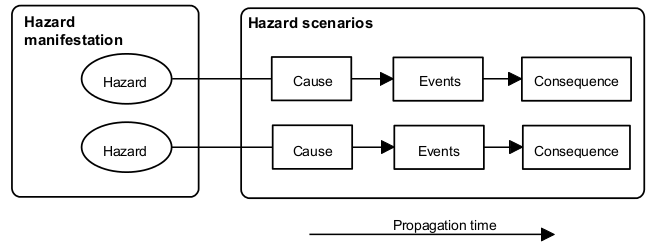
\includegraphics[scale=0.6]{fig/example_of_hazards_and_hazard_scenarios}
\caption{Example of Hazards and Hazard Scenarios (copyright ECSS)}
\label{fig:Example of Hazards and Hazard Scenarios}
\end{figure}

Hazards are reduced by either eliminating them or, if not feasible, by minimizing and controlling them (see Figure \ref{fig:Removal or Change of Hazards, Elimination of Event, or Interruption of Event}). 

\begin{figure}[h]
\centering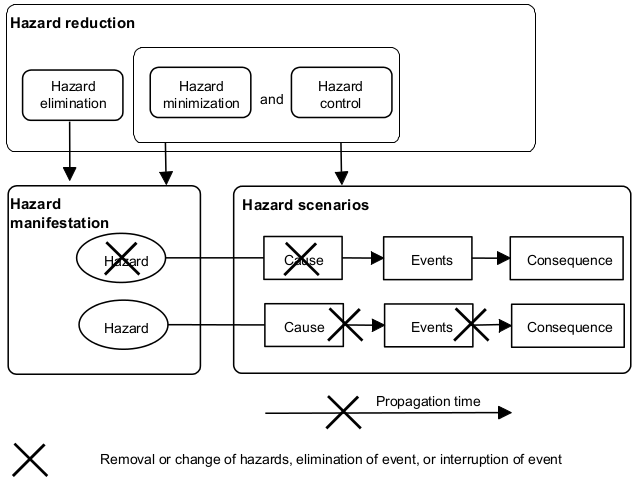
\includegraphics[scale=0.6]{fig/removal_or_change_of_hazards}
\caption{Removal or Change of Hazards, Elimination of Event, or Interruption of Event (copyright ECSS)}
\label{fig:Removal or Change of Hazards, Elimination of Event, or Interruption of Event}
\end{figure}

\subsubsection{Fault Tree Analysis}

\begin{tabular}{l}
\textit{ECSS-Q-ST-40-12 "Fault tree analysis" \cite{ECSS-Q-ST-40-12}}
\end{tabular}

Fault tree analysis (FTA) is a top-down method that stipulates a fault and tries to identify causes to led to this fault. This is done downwards the system levels until the root causes are found. This is in contrast with failure mode and effects analysis (FMEA), which is an inductive, bottom-up analysis method aimed at analyzing the effects of single component or function failures on the next higher system. 

\begin{figure}[h]
\centering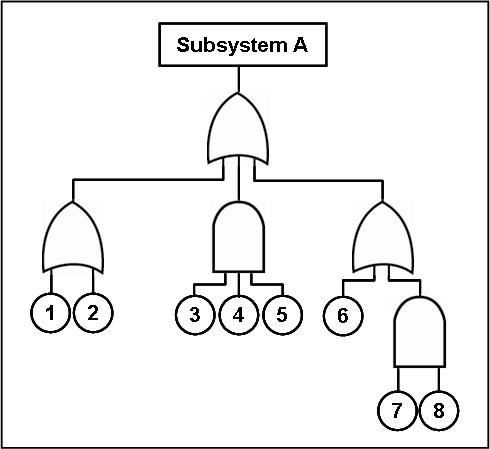
\includegraphics[scale=1.0]{fig/example_of_fault_tree_analysis}
\caption{Example of Fault Tree Analysis}
\label{fig:Example of Fault Tree Analysis}
\end{figure}

\subsubsection{Space Sustainability}

Safety is related to space sustainability through debris mitigation and atmospheric re-entry considerations. The system design and operation shall be such as to minimize \textbf{debris mitigation}, which pose a potential collision hazard to other objects in space. See ECSS-U-AS-10 \cite{ECSS-U-AS-10} for an adoption note of the ISO 24113 standard on space debris mitigation requirements. \textbf{Atmospheric re-entry} on the other hand poses a risk to people, environment, and property. For CubeSats, re-entry issues are not of concern, due to its low mass and size.

\subsection{EEE Components}

The electrical, electronic and electromechanical (EEE) components discipline defines some specific requirements for selection, control and procurement of EEE components for space projects to ensure that they satisfy the mission performance requirements during the full life cycle of the products.  

ECSS-Q-ST-60 \cite{ECSS-Q-ST-60} differentiates between three classes of components, from class 1 with highest assurance and lowest risk, to class 3 with lowest assurance and highest risk. The standard then defines the requirements for components of those three classes. ECSS-Q-ST-60-13 \cite{ECSS-Q-ST-60-13} extends this standard further, by tailoring and modifying its requirements with application to commercial off-the-shelf (COTS) components. 

For typical CubeSat missions even class 3 requirements are in most cases much too demanding. Nonetheless, it is good practice to check against the availability of space qualified components, such as published at the website of the European Space Components Information Exchange System (ESCIES) \cite{escies.org}. 

Further, a \textbf{declared component list} (DCL) (Template \ref{app:Declared Component List}) shall be maintained that provides a status list of all the EEE components intended to be used or actually used in the system.

As mentioned, mainly COTS EEE components are employed in CubeSat missions. For designs that implement such components of which some or all are not space qualified (i.e. they do not carry heritage from flown space missions), the following aspects shall be taken into special account: 

\begin{itemize}
\item \textbf{Temperature range}: Commercial parts shall be selected in the highest available temperature range and shall have a minimum margin of $10\,^{\circ}\mathrm{C}$.
\item \textbf{Radiation}: Survival and successful operation of space systems in the space radiation environment cannot be ensured without careful consideration of the effects of radiation, namely the effects of total ionizing dose (TID), total non-ionizing dose (TNID) and single-event effects (SEE). ECSS-Q-ST-60-15 \cite{ECSS-Q-ST-60-15} provides details on radiation hardening assurance. ECSS-E-HB-10-12 \cite{ECSS-E-HB-10-12} provides details on calculation of radiation and its effects.
\end{itemize}

\subsection{Materials, Parts and Processes}

\begin{tabular}{l}
\textit{ECSS-Q-ST-70 "Materials, mechanical parts and processes" \cite{ECSS-Q-ST-70}}
\end{tabular}

The materials, mechanical parts and processes discipline defines requirements for selection, control and procurement of materials, mechanical parts and processes for space projects to ensure that they satisfy the mission performance requirements during the full life cycle of the products. 

The following lists are to be prepared and maintained for all the configuration items in the system:

\begin{itemize}
\item \textbf{Declared materials list (DML)}: A detailed record of all the materials used to produce the products of the space system. To obtain this list, one may need to access the composition of parts in terms of materials (Template \ref{app:Declared Materials List}).
\item \textbf{Declared mechanical parts list (DMPL)}: A detailed record of all the mechanical parts used to produce the products of the system. The bill of material (BOM) of products can be used to derive this information (Template \ref{app:Declared Mechanical Parts List}).
\item \textbf{Declared process list (DPL)}: A detailed record of all the processes used to produce the products of the space system (Template \ref{app:Declared Process List}).
\end{itemize}

A helpful guideline for the selection of materials and definition of processes is provided in ECSS-Q-ST-70-71 \cite{ECSS-Q-ST-70-71}.

\subsubsection{Cleanliness}

\begin{tabular}{l}
\textit{ECSS-Q-ST-70-01 "Cleanliness and contamination control" \cite{ECSS-Q-ST-70-01}}
\end{tabular}

The purpose of cleanliness and contamination control is to avoid malfunctions and failures of hardware items due to particulate or molecular contamination. The classification of \textbf{particulate contamination levels} is done in ISO Class levels from 1 to 9, with ISO Class level 1 being the cleanest. The levels specify the maximum concentration of particles of different sizes per air volume.

The requirements on \textbf{cleanrooms} are provided in detail and govern the design aspects of the cleanroom, the air supply, the filters, the air monitoring, the temperature control, the pressure control, and the humidity control. It also specifies on how to verify the cleanroom cleanliness levels. The maintenance, cleaning, and access control to the cleanroom are specified as well. ECSS-Q-ST-70-50 \cite{ECSS-Q-ST-70-50} provides more detail on \textbf{monitoring of contamination} for space systems and cleanrooms.

Appendix D and E of ECSS-Q-ST-70-01 provide guidelines for \textbf{general cleanliness and contamination control} and on \textbf{cleanliness-oriented design}. Appendix I of ECSS-Q-ST-70-01 provides an matrix of compatibility of \textbf{cleaning solvents} and target materials. Appendix M of ECSS-Q-ST-70-01 provides an informative guide on \textbf{cleaning methods} for removal of particulate and molecular contamination.

\subsubsection{Material Testing}

Several ECSS standards cover the details of testing of various (basic) materials (not including assemblies or electronic components). It shall be noted that those tests are usually not carried out for a typical CubeSat project, unless specifically required.

\begin{itemize}
\item \textbf{Outgassing}: Thermal vacuum tests as described in ECSS-Q-ST-70-02 \cite{ECSS-Q-ST-70-02} and ECSS-Q-TM-70-52 \cite{ECSS-Q-TM-70-52} are used to determine the outgassing screening properties of materials proposed for use in space. The focus is on determining the the values of total mass loss (TML), recovered mass loss (RML), and collected volatile condensable material (CVCM) of a specimen. It describes the requirements on the test preparation and equipment, the test procedure and test levels.
\item \textbf{Thermal cycling}: The objective of thermal cycling testing is to determine the ability of articles to withstand changes of ambient temperature under vacuum. The specimen are subjected to a certain number of thermal cycles, oscillating within a defined temperature range, as specified in ECSS-Q-ST-70-04 \cite{ECSS-Q-ST-70-04}.
\item \textbf{Radiation}: The testing of specimen exposed to electromagnetic radiation and charged particles is described in ECSS-Q-ST-70-06 \cite{ECSS-Q-ST-70-06}. 
\item \textbf{Corrosion}: Although ECSS-Q-ST-70-20 \cite{ECSS-Q-ST-70-20} is focused on corrosion tests of silver-plated copper wire and cables, it also is a good guideline on general corrosion tests.
\item \textbf{Flammability}: All non-metallic materials are inherently flammable, the degree to which this is true is dependent on the chemical nature of the material itself and the environment to which the material is exposed. Flammability tests as discussed in ECSS-Q-ST-70-21 \cite{ECSS-Q-ST-70-21} play an important role for manned missions, but not so for CubeSat missions.
\item \textbf{Offgassing}: All non-metallic materials release trace contaminants into the surrounding environment, the extent to which this occurs is dependent on the nature of the material concerned. Offgassing test as discussed in ECSS-Q-ST-70-29 \cite{ECSS-Q-ST-70-29} are of importance to manned missions, but not so for CubeSat missions.
\item \textbf{Cracking}: Certain materials are more susceptible to stress corrosion cracking (SCC) than others. If a susceptible material is placed in service in a corrosive environment under tension of sufficient magnitude, and the duration of service is sufficient to permit the initiation and growth of cracks, failure occurs at a stress lower than that which the material is normally be expected to withstand. ECSS-Q-ST-70-36 \cite{ECSS-Q-ST-70-36} provides information on material selection to reduce and control SCC, whereas ECSS-Q-ST-70-37 \cite{ECSS-Q-ST-70-37} provides details determination of SCC susceptibility of metals.
\item \textbf{Metallic properties}: The most relevant test methods for mechanical testing of metallic materials to assess the tensile, fatigue and fracture properties are discussed in ECSS-Q-ST-70-45 \cite{ECSS-Q-ST-70-45}.
\end{itemize}

\subsubsection{Material Processes}

Several ECSS standards cover the details of processes applied on material level. Depending on the mission requirements, some of them may be of importance to a CubeSat project.

\begin{itemize}
\item \textbf{Anodizing}: Passive thermal control systems are often based on the thermo-optical properties of surfaces. ECSS-Q-ST-70-03 \cite{ECSS-Q-ST-70-03} specifies how to conduct proper black-anodizing of metallic surfaces through controlled oxidation with inorganic dyes.
\item \textbf{Thermo-optical measurement}: The thermo-optical properties of materials are of importance for the calculation of thermal housekeeping and radiative heat transfer. ECSS-Q-ST-70-09 \cite{ECSS-Q-ST-70-09} specifies the procedures and instrument requirements to conduct measurements of solar absorptance and infrared emittance.
\item \textbf{Peel and pull-off strength measurement}: The quality of adhesion of coatings, paints, files, etc. on spacecraft equipment is affected by exposure to the environment. ECSS-Q-ST-70-13 \cite{ECSS-Q-ST-70-13} specifies measurement requirements and procedures for using pressure-sensitive tapes to access such adhesion quality.
\item \textbf{Control of shelf-life}: For materials that depend on a chemical reaction for their application, the properties of the reactants are of importance. Those properties are influenced by age and storage condition. ECSS-Q-ST-70-22 \cite{ECSS-Q-ST-70-22} specifies how to store and control such materials with limited shelf-life.
\item \textbf{Application of paints}: The generic preparation and application procedure for paints on spacecraft hardware is detailed in ECSS-Q-ST-70-31 \cite{ECSS-Q-ST-70-31}.
\end{itemize}

\subsubsection{Assembling Processes}

Several ECSS standards cover the details of (lower level) assembly processes. Most of them are of importance to a CubeSat project.

\begin{itemize}
\item \textbf{Soldering}: The soldering of components on printed circuit boards is most often done manually by hand. This is due to the small number of identically designed circuits in a project that could warrant the setting up of unique machine parameters for each individual layout. Nonetheless, for boards that were produced using automated wave soldering, ECSS-Q-ST-70-07 \cite{ECSS-Q-ST-70-07} provides requirements for verification and approval. ECSS-Q-ST-70-08 \cite{ECSS-Q-ST-70-08} on the other hand provides detailed information and procedures for carrying out high reliable manual soldering. ECSS-Q-ST-70-38 \cite{ECSS-Q-ST-70-38} further extends this to the soldering of high-reliability electronic circuits based on surface mount devices (SMD) and mixed technology.
\item \textbf{Crimping}: The requirements for and approval conditions of crimped wired terminations are discussed in ECSS-Q-ST-70-26 \cite{ECSS-Q-ST-70-26} in detail for single and multiple wire contacts, coaxial connectors, and lugs and splices.
\item \textbf{PCB repair and modifications}: The requirements and procedures for repair and modification of single-sided, double-sided, and multi-layer printed circuit boards are detailed in ECSS-Q-ST-70-28 \cite{ECSS-Q-ST-70-28}.
\item \textbf{Wire wrapping}: The production of wire-wrapped connections is a relatively simple yet precision method of fusion. Its use for high reliability space conditions affords high skills and is discussed in ECSS-Q-ST-70-30 \cite{ECSS-Q-ST-70-30}.
\item \textbf{Welding}: The welding of metallic parts for CubeSats is rarely, if at all, a topic of concern. Nonetheless, ECSS-Q-ST-70-39 \cite{ECSS-Q-ST-70-39} provides necessary requirements for it. 
\end{itemize}

\subsubsection{Parts}

Several ECSS standards cover the details of items on parts level. (A part is a set of materials, assembled according to defined and controlled processes, which cannot be disassembled without destroying its capability and which performs a simple function that can be evaluated against expected performance requirements). Most of those standards are of importance to a CubeSat project.

\begin{itemize}
\item \textbf{Printed circuit boards}:  A number of ECSS standards are concerned with printed circuit boards (PCBs). ECSS-Q-ST-70-10 \cite{ECSS-Q-ST-70-10} specifies requirements for evaluation and qualification of PCBS procured from a manufacturer. ECSS-Q-ST-70-11 \cite{ECSS-Q-ST-70-11} extends this to cover the procurement process of PCBs from a manufacturer. Although both standards are rarely needed for CubeSat projects, they still provide good insight about important characteristics of a PCB. A very detailed and helpful guide is ECSS-Q-ST-70-12 \cite{ECSS-Q-ST-70-12}, which provides a large number of \textbf{design rules} for PCBs. It covers rigid, flex, and rigid-flex PCBs, and takes into account thermal, RF, and electrical design aspects.
\item \textbf{RF coaxial cables}: For transmission lines of radio signals with frequencies up to the microwave region, ECSS-Q-ST-70-18 \cite{ECSS-Q-ST-70-18} provides details on assembly and mounting of such coaxial-cable interconnections.
\end{itemize}

\subsection{Software Product Assurance}

\begin{tabular}{l}
\textit{ECSS-Q-ST-80 "Software product assurance" \cite{ECSS-Q-ST-80}}
\end{tabular}

The software product assurance discipline defines requirements to ensure that developed or reused software and software services perform properly and safely in their operational environments. It also includes requirements for the development of supporting software (e.g. for test and verification) which affects the quality of the deliverable product or service.

In a system of systems, a software product can be considered to constitute a system itself, whether it is firmware embedded in a microcontroller or data systems running on personal or industrial computers. Being a system, all aspects of management, product assurance, and engineering apply equally to it, as to they do to the overall space system of which it is part. It makes therefore a difference whether the software development is carried out in the frame of the project or implemented as an autonomous software project, which is then (re)used for the particular CubeSat project.

For an autonomous, \textbf{standalone software project}, ECSS-Q-ST-80 together with ECSS-E-ST-40 \cite{ECSS-E-ST-40} provide all the framework requirements for its implementation, covering the entire life cycle from requirements definition, architectural design, software items design, coding, testing and validation, operation, and maintenance. The use of such independently developed software in the CubeSat project would then only require the application of the terms governing the reuse of existing software as detailed in ECSS-Q-ST-80.

For \textbf{integrated software projects} on the other hand, developed as part of the space project, many of the management and product assurance aspects can be shared within the project. For example, software risk management can be part of the overall project risk management. Also, the software product assurance plan, may be integrated into the overall product assurance plan. 

Nonetheless, for CubeSat projects we recommended to pursue software project (in particular those that are not firmware projects) as independent projects, decoupled from the specific CubeSat mission. This way it enforces re-usability of software and it allows the selection of a different development approach, such as agile development. 

Either way, the following two documents shall be prepared and maintained by the product assurance manager. The \textbf{software product assurance plan} (Template \ref{app:Software Product Assurance Plan}) defines all the product assurance aspects of the software development (as mentioned, this one may be merged into the overall product assurance plan). The \textbf{software product assurance milestone report} (Template \ref{app:Software Product Assurance Milestone Report}) is used to report on software product assurance activities that were performed during the past project phase.

\clearpage
\section{Deliverables}
\label{sec:Product Assurance Deliverables}

\subsection{Documents per Review}
\begin{table}[h]
\centering
\begin{tabular}{l c c c c c c c c c}
\toprule
\textbf{Phase} & \textbf{0} & \textbf{A} & \multicolumn{2}{c}{\textbf{B}} & \textbf{C} & \multicolumn{2}{c}{\textbf{D}} & \multicolumn{2}{c}{\textbf{E}} \\
\textbf{Review} & \textbf{MDR} & \textbf{PRR} & \textbf{SRR} & \textbf{PDR} & \textbf{CDR} & \textbf{QR} & \textbf{AR} & \textbf{ORR} & \textbf{FRR} \\
\midrule
Product assurance plan     		&   &(•)&(•)& • & • &   &   & o &   \\
\hline
Critical-item list				&   &   &(•)& • & • & • & • &   & • \\
\hline
Qualification status list 		&   &(•)&   & • & • & • & • &   &   \\
\hline
Quality assurance plan          &   & • & • & • & • &   &   &   &   \\
\hline
End item data package           &   &   &   &   &   & • & • &   &   \\
\hline
Safety program plan             &   & • & • & • & • & • & • & • & • \\
\hline
Declared component list         &   &   &   & • & • & • & • &   &   \\
\hline
SW PA plan                      &   &   & • & • & • & • & • & • &   \\
\hline
SW PA milestone report          &   &   & • & • & • & • & • & • &   \\
\bottomrule
\end{tabular}
\caption{Product assurance required per Review}
\end{table}

\begin{tabular}{l l}
(•) &= Preliminary \\
o &= covering operational phase
\end{tabular}


\chapterimage{chapter_head_01} % Chapter heading image
\chapter{Engineering}

\section{Overview}

Next to project management and product assurance, engineering is the third branch of a space project. And it is the most essential one, as it produces the actual product or artefact, which is to achieve/deliver the mission objectives. In fact, project management and product assurance are merely functions (but very important one) that support and guide the engineering process. In this chapter we have a detailed look on the various aspects of engineering a space product.

\section{Engineering Disciplines}

In order to implement the system engineering process, a number of system engineering disciplines are involved. They are described in the following sections.

\subsection{System Engineering}
\label{sec:System Engineering}

\begin{tabular}{l}
\textit{ECSS-E-ST-10 "System engineering general requirements" \cite{ECSS-E-ST-10}}
\end{tabular}

System engineering is a multidisciplinary activity that transforms all technical requirements of the system into a system solution. A system is defined as an integrated set of elements to accomplish a defined objective. These elements include hardware, software, firmware, human resources, information, techniques, facilities services, and other support elements.

The concept of "system" is used here in a wide sense. The highest level, often called "mission level" or "space system", consists usually of one (or more) space segment(s), a ground segment, a launch segment, and a user segment. Elements of system decomposition are also considered a system. Hence, a system can be any element at any level of decomposition as defined by the function tree or the product tree. The scope of an element can include hardware, software, procedures, facilities and services.

The overall objective of system engineering is to obtain a product that satisfies the customer technical requirements within defined budget and time constraints. It includes the activities of definition of requirements, analysis, design and development, and verification. This is applied on all levels of the system. 

The governing document for all the system engineering activities is the \textbf{system engineering plan} (Section \ref{sec:System Engineering Plan}. The SEP gets input from other disciplines, including project management, product assurance, other engineering disciplines, production, operations and logistics. The SEP is continuously updated through the course of the project.

The traditional approach for conducting space system engineering is the waterfall approach, at which the following processes are carried out subsequently (corresponding to the project phases): definition of requirements, system design and production, and system verification.

\subsubsection{Requirements Engineering}

Requirements define the required technical performance of the system. Requirements are established on all levels of the system, and usually are elaborated from top to bottom. For example, a single high level requirement may be split into a number of low level requirements. This is done recursively until requirements on the lowest level are defined. To visualize the requirements, a specification tree may be used. However, to keep the tree manageable, the equipment element level requirements (and below) are usually put on a separate tree.

It must be ensured that requirements are consistent on all levels, that is, that they not contradict one another. Each requirement must be have the characteristics of being: traceable, unique, single, verifiable, unambiguous.

For being \textbf{traceable}, it must be clear from where the requirement originates, e.g. from a higher level requirements, an imposed constraint, and so on. For this, a requirement traceability matrix is used. For being \textbf{verifiable}, one or more methods must be identified for each requirement that will be used for its verification. \textbf{Unique} means that there must not be duplicated requirements, and \textbf{single} means that a requirement shall only cover one specific performance characteristic. \textbf{Unambiguous} means that requirements shall be written in a clear and precise way that leaves no room for interpretation.

There are several types of requirements, of which all or a subset may be applicable to the system element under consideration. ECSS-E-ST-10-06 \cite{ECSS-E-ST-10-06} provides details on the different requirements types and how to adequately define requirements. The list of requirements shall then be compiled in a \textbf{technical requirements specification} (Section \ref{sec:Technical Requirements Specification}). 

The source of requirements are manifold. For each project there are mission and project specific requirements. In addition, there is also a large number of generic requirements. Many requirements originate from mission analysis, which includes among others the analysis of the \textbf{space environment} (ECSS-E-ST-10-04 \cite{ECSS-E-ST-10-04} provides environmental models). Also non-technical factors, such as programmatic or product assurance constraints influence the system design. Generic requirements originate from applicable standards and expectations of common functionality and performance (ECSS-E-70-11 \cite{ECSS-E-ST-70-11} provides requirements on space segment operability).

Another important set of requirements are interface requirements. They are established with the objective to achieve functional and physical compatibility amongst all interrelated items in the product tree. ECSS-E-ST-10-24 \cite{ECSS-E-ST-10-24} provides a detailed list of reference interface data as a baseline for a \textbf{interface requirements document} (which itself is part of the technical requirements specification). 

Requirements are collected in a requirements database and by all means should not be changed after the completion of the requirements definition phase. A late change of requirement (e.g. during production phase) will likely incur high costs.

\subsubsection{Analysis}

Analysis is performed for decomposition of requirements and functional requirements analysis, resolving requirement conflicts, and estimating system performance. It is used to support the requirements engineering and the design process.

As an input to requirement engineering, the system engineering team shall perform an analysis of the \textbf{mission statement document} (Section \ref{sec:Mission Statement Document}) to produce the \textbf{mission description document} (Section \ref{sec:Mission Description Document}). For the case where several mission scenarios shall be compared and traded-off with each other, separate mission description documents, together with system engineering and project management plans are created. The winning concept is then chosen and document in a \textbf{system concept report} (Section \ref{sec:System Concept Report}).

Next, the functional architecture shall be established in form of a \textbf{function tree}. The function tree shall satisfies the customer requirements in terms of functionality, that is, the mission objective shall be composed into functional requirements.

In support of the design process, the system engineering team performs physical analysis to produce the \textbf{physical architecture} and the \textbf{product tree} (see Figure \ref{fig:Example of Product Tree}) of the system. Analysis is further used to justify the selected physical architecture. This includes a very wide range of analyses, such as thermal analysis, attitude and orbit analysis, data link analyses, etc. Performance analysis is to be performed on various levels of the system architecture, including end-to-end evaluation of the complete system. Analysis may also be performed to identify the impact of system imposed constraints to the cost and schedule of the project. 

All analyses are to be documented in analysis reports (Section \ref{sec:Analysis Report}).

\subsubsection{Design}

The design and development process produces a physical architecture of the complete system in terms of functionality and all the hardware and software characteristics.

The two main artifacts produced by the system engineering team are the \textbf{design definition file} (Section \ref{sec:Design Definition File}) and the \textbf{design justification file} (Section \ref{sec:Design Justification File}). Both are data repositories that hold references to all the information produced during the system design process. 

The design definition file (DDF) covers the technical definition of the system or product that complies with its technical requirements specification. The main aspects of the DDF are:

\begin{itemize}
\item Functional description (functional architecture, function tree, function chains)
\item Physical description (physical architecture, product and specification tree, element and interface description, technical budgets, margins, deviations)
\item Design constraints (constraints related to production, logistics, operation, maintainability)
\end{itemize}

The interfaces of the system are maintained in a dedicated \textbf{interface control document} for each interface (Section \ref{sec:Interface Control Document}) 

The design justification file (DJF) on the other hand is used to represent the rationale for the selected design solution, and to demonstrate that the design meets the requirements. The main aspects of the DJF are:

\begin{itemize}
\item Justification of functional architecture
\item Justification of physical architecture
\item Verification activities and reports
\item Justification of system budgets and margins
\item Justification of constraints imposed by system design
\end{itemize}

During the design process the system engineering team is working on the establishment and maintenance of the design definition file and the design justification file, and produces a \textbf{product user manual} (Section \ref{sec:Product User Manual}) that provides information on the design, operations, and data of the system that is required by the user to handle, install, operate, maintain, and dispose the product during its life time. If the system is a space segment, the product user manual (PUM) to produce is called \textbf{space segment user manual} (SSUM) (Section \ref{sec:Space Segment User Manual}).

Other supporting documents are the technical budget document and the coordinate system document. The \textbf{technical budget document} (Section \ref{sec:Technical Budget Document}) contains the various technical budgets of the system and may also record the evolution of the budgets over time. The \textbf{coordinate system document} (Section \ref{sec:Coordinate System Document}) is used to establish the reference coordinate systems to be used throughout the project.

\subsubsection{Verification}
\label{sec:Verification}

\begin{tabular}{l}
\textit{ECSS-E-ST-10-02 "Verification" \cite{ECSS-E-ST-10-02}} \\
\textit{ECSS-E-HB-10-02 "Verification guidelines" \cite{ECSS-E-HB-10-02}}
\end{tabular}

Verification has the objective to demonstrate that the deliverable products conform to the specified requirements. The verification process activities consist of planning, execution, and reporting and close-out. 

The verification planning is documented in the \textbf{verification plan} (Section \ref{sec:Verification Plan}) and covers the verification approach,model philosophy, methods, levels, stages, and verification tools. 

The \textbf{verification approach} activity is started early in the project life cycle. It analyzes which, how, and when requirements shall be verified, taking into account constraints and other factors. For each requirement to be verified, the verification strategy shall be defined in terms of verification methods, level, and stages. This is summarized in the \textbf{verification control document} (Section \ref{sec:Verification Control Document}) also known as verification matrix, which is to be approved by the customer.

The \textbf{model philosophy} defines the physical models that are required to achieve confidence in the product verification. The philosophy to be chosen depends on several factors, such as risk level, heritage, programmatic constraints, and budget. There are two dominant philosophies: prototype and protoflight. In the first approach separate models for qualification and acceptance are produced, whereas in the protoflight approach one model undergoes both verification stages. Hence the protoflight approach is cheaper but more risky, and suitable for systems with flight heritage.

The usual approach for new developments is therefore the prototype philosophy. An example of such a prototype philosophy and the associated models is shown in Figure \ref{fig:Example of Prototype Philosophy}.

\begin{figure}[h]
\centering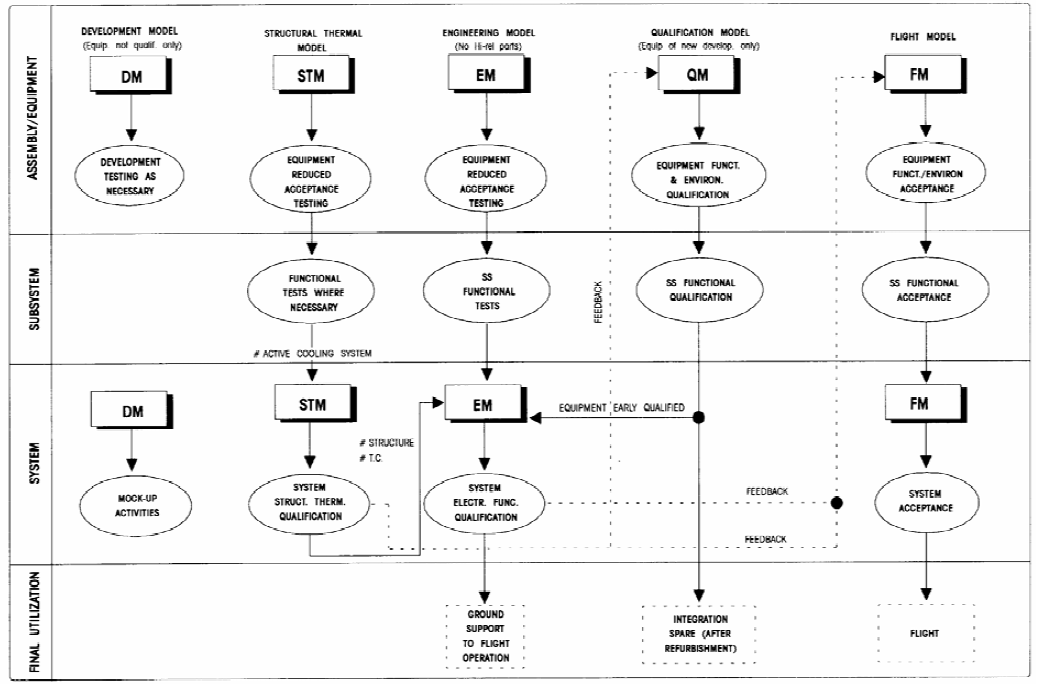
\includegraphics[scale=0.4]{fig/example_of_prototype_philosophy}
\caption{Example of Prototype Philosophy (ECSS)}
\label{fig:Example of Prototype Philosophy}
\end{figure}

Commonly defined models for verification programs are:

\begin{itemize}
\item \textbf{Development model} (DM): Used in general for new design or when substantial redesign is performed. Applicable to every type of product (e.g. electronic box, mechanisms, structural parts and thermal equipment) and can be subjected to functional and/or environmental testing. DM are sometimes also called bread board model.
\item \textbf{Structural model} (SM): Fully representative of the end product for structural aspects. Used for qualification of the structural design and for mathematical models correlation. Generally, the system structural model consists of a representative structure, with structural dummies of the flight equipment. It also includes representative mechanical parts of other subsystems (e.g. mechanisms and solar panels). The SM is also used for a final validation of test facilities, GSE, and related procedures.
\item \textbf{Thermal model} (ThM): Fully representative of the thermal properties of the end product. Used for the qualification of the thermal design and for the correlation of mathematical models. 
\item \textbf{Structural-thermal model} (STM): Combines the objectives of the SM and ThM.
\item \textbf{Suitcase model} (ScM): Intended to be used with the ground station for verifying correct telemetry (TM) reception, telecommand (TC) commanding. It is representative of the RF receiver and transmitter as well as the data handling part involved in the TM/TC protocol. 
\item \textbf{Electrical and functional model} (EFM): Functionally representative of the end products in both electrical and software terms. They are used for functional and interface tests and for failure mode investigations. Some part can be simulated by software; the rest is using commercial parts. Also known as Flatsat.
\item \textbf{Engineering model} (EM): Flight representative in form, fit and function, without high reliability parts and usually without full redundancy. The EM is used for functional qualification and failure survival demonstration. The EM is also used for final validation of test facilities and GSE and the related procedures.
\item \textbf{Qualification model} (QM): Fully reflects the end product design in all aspects. The QM is
used for complete functional and environmental qualification tests. 
\item \textbf{Flight model} (FM): The flight end product. It is subjected to formal functional and environmental acceptance testing. 
\item \textbf{Flight spare} (FS): The spare end product for flight. It is subjected to formal acceptance testing.
\end{itemize}

The \textbf{verification methods} available to the verification engineer are:

\begin{itemize}
\item Test
\item Analysis
\item Review of design
\item Inspection
\end{itemize}

The list is ordered by the magnitude of confidence that each verification methods gives, with tests being the most reliable verification methods. Hence, all (safety) critical functions shall be verified by test.

\textbf{Tests} shall be conducted under representative simulated environments. Tests objectives shall be documented via a \textbf{test specification} (Section \ref{sec:Test Specification}), the test conduction via a \textbf{test procedure} (Section \ref{sec:Test Procedure}) and the test results via \textbf{test report} (Section \ref{sec:Test Report}). The overall test program encompassing all tests shall be defined in the \textbf{assembly, integration, and test plan} (Section \ref{sec:Assembly, Integration, and Test Plan}).

\textbf{Analyses} use either theoretical or empirical techniques, such as statistical analysis or computational simulation. Analysis also covers verification by similarity. Analyses are document in the \textbf{analysis report} (Section \ref{sec:Analysis Report}).

\textbf{Review of design} uses records or evidence (such as technical drawings) that show unambiguously that a requirement is met. Reviews of design are document in the \textbf{review of design report} (Section \ref{sec:Review of Design Report}).

\textbf{Inspection} consists of visual determination of physical characteristics. Examples are visual inspection of products against workmanship errors or checking the conformance of source code against the defined \textbf{coding standards}. Inspections are document in the \textbf{inspection report} (Section \ref{sec:Inspection Report}).

In case that a verification encompasses more than one of the above methods, a \textbf{verification report} (Section \ref{sec:Verification Report}) is produced in addition to the other types of reports.

Verification shall be accomplished through selected \textbf{verification levels}. The verification process proceeds from lower level to higher level, i.e. the overall space system is verified last. Usual verification levels are:

\begin{itemize}
\item Space system (= mission)
\item Segment (e.g. ground segment, space segment)
\item Element (e.g. spacecraft platform)
\item Subsystem (e.g. AOCS)
\item Equipment (e.g. star tracker)
\end{itemize}

The verification process runs through several subsequent \textbf{verification stages}, which are:

\begin{itemize}
\item Qualification
\item Acceptance 
\item Pre-launch
\item In-orbit
\item Post-landing (if applicable)
\end{itemize}

In the \textbf{qualification stage} the verification shall demonstrate that the design, including margin, meets the applicable requirements. Therefore the product to be verified must be representative of the end product in terms of design, materials, tooling, and methods. To decide which item to be verified for the qualification test the general rule is that newly developed items must undergo full qualification, whereas items with heritage must undergo no or delta qualification, depending on their heritage.

In the \textbf{acceptance stage} the verification shall demonstrate that the product is free of workmanship errors and that it is ready for operation. Acceptance verification is carried out on the final product. 

In the \textbf{pre-launch stage} the verification shall demonstrate that the product is ready for launch and early operations.

In the \textbf{in-orbit stage} the verification shall ensure that no degradation occurred during launch and early operations. This stage also serves to confirm the space and ground segment inter-operability and operational aspects that cannot be verified before launch. Further, during this stage the spacecraft payload is calibrated and tuned for operation.

Typical \textbf{verification tools} are: 

\begin{itemize}
\item Ground support equipment (GSE)
\item Software validation facility (SVF)
\item Simulators
\item Software tools for analyses
\item Integration and test facilities
\end{itemize}

\subsubsection{Testing}

\begin{tabular}{l}
\textit{ECSS-E-ST-10-03 "Testing" \cite{ECSS-E-ST-10-03}}
\end{tabular}

Although testing is part of the verification program, it is of such importance to the system development that it is elaborated in more detail in this section. On the other hand, the discussion here is focused on testing of system elements from equipment up to segment level but not about testing of the overall system (e.g. end-to-end test or system validation test). To be more exact, this section is concerned with testing of qualification and flight (including protoflight) models.

Testing is conducted in the qualification, acceptance, and pre-launch stages of the verification process, and normally applied subsequently from lower level to higher level system elements. That means that in the qualification stage, qualification testing is carried out with individual equipment, which is then assembled and tested on subsystem level, and so on. Only when all testing related to the qualification stage has been completed one moves to the testing related to the acceptance stage.

Different testing requirements are applied for space segment equipment (e.g. processing modules, actuators, sensors) and space segment elements (the assembled spacecraft model). 

The \textbf{test planning} comprises of the establishment of the test program and the test reviews. The test program is decomposed into \textbf{test blocks} covering one specific test aspect and may contain one or more individual tests. Each test block is accompanied by \textbf{test reviews}, namely a \textbf{test readiness review} (TRR) to verify before the start of the test activity that all conditions allow to proceed with the test, and a \textbf{post test review} (PTR) to formally declare the test completed. 

The \textbf{test documentation} comprises of the \textbf{assembly, integration and test plan}, the individual \textbf{test specifications}, \textbf{test procedures}, \textbf{test reports}, and all the test data. Tests that are not passed are subject to nonconformance control.
 
The \textbf{test conditions} shall be such as to resemble predicted environments plus margin. Further, aspects of product assurance, namely safety and cleanliness, shall be implemented. \textbf{Test tolerances} and \textbf{ test accuracies} shall be agreed with the customer. Recommended values for tolerances and accuracies are provided in ECSS-E-ST-10-03 \cite{ECSS-E-ST-10-03}.

\textbf{Testing of equipment} typically comprises the following test blocks (although not all tests are applicable to all equipment):

\begin{itemize}
\item General tests
	\begin{itemize}
	\item Functional and performance: full test of all functionality (including deployments), system modes, and performance.
	\item Humidity (if applicable): functional test under humidity.
	\item Life (if applicable): test life time of life limited equipment.
	\end{itemize}
\item Mechanical tests
	\begin{itemize}
	\item Physical properties: determine dimensions, interfaces, mass, CoG, and MoI of equipment in launch configuration.
	\item Acceleration
	\item Random vibration
	\item Acoustic
	\item Sinusoidal vibration
	\item Shock
	\end{itemize}
\item Structural integrity tests
	\begin{itemize}
	\item Leak (if applicable): to be conducted before and after pressure, thermal, and mechanical tests of pressurized or sealed equipment.
	\item Proof pressure and pressure cycling (if applicable)
	\end{itemize}
\item Thermal tests
	\begin{itemize}
	\item Thermal vacuum
	\end{itemize}
\item Electrical/RF tests
	\begin{itemize}
	\item Electromagnetic compatibility
	\item Magnetic
	\item ESD
	\end{itemize}
\item Mission specific tests
\end{itemize}

Equipment test details and test levels for qualification and acceptance can be found in ECSS-E-ST-10-03 \cite{ECSS-E-ST-10-03} as well. An example of a full test sequence for equipment is shown in Figure \ref{fig:Example of Equipment Test Sequence}. 

\begin{figure}[h]
\centering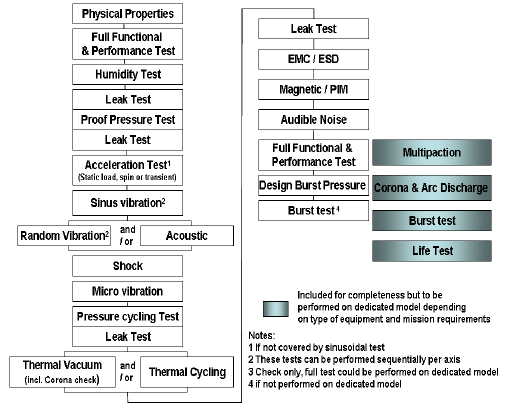
\includegraphics[scale=0.7]{fig/example_of_equipment_test_sequence}
\caption{Example of Equipment Test Sequence (ECSS)}
\label{fig:Example of Equipment Test Sequence}
\end{figure}

\textbf{Testing of spacecraft model} is to a large degree dependent on mission requirements and launcher profile. The following lists typical test blocks to be completed on spacecraft level, unless the launch provider requires different tests and/or test levels:

\begin{itemize}
\item General tests
	\begin{itemize}
	\item Functional (mechanical and electrical) and performance
	\item Mission: simulate nominal and contingency scenarios.
	\end{itemize}
\item Mechanical tests
	\begin{itemize}
	\item Physical properties: determine mass, CoG, and MoI of spacecraft in launch and orbit configuration.
	\item Modal survey
	\item Static load
	\item Spin
	\item Transient
	\item Acoustic
	\item Random vibration
	\item Sinusoidal vibration
	\item Shock
	\end{itemize}
\item Structural integrity tests
	\begin{itemize}
	\item Leak (if applicable)
	\item Proof pressure and pressure cycle (if applicable)
	\end{itemize}
\item Thermal tests
	\begin{itemize}
	\item Thermal vacuum
	\item Thermal balance
	\end{itemize}
\item Electrical/RF tests
	\begin{itemize}
	\item Electromagnetic compatibility
	\item Magnetic filed measurements
	\end{itemize}
\item Mission specific tests
\end{itemize}

Again, the test details and test levels for qualification and acceptance on spacecraft level can be found in ECSS-Q-ST-10-03 \cite{ECSS-E-ST-10-03}.

\textbf{Pre-launch testing} is very specific to the spacecraft and comprises at a minimum:

\begin{itemize}
\item Functional testing to verify that no damage or degradation has occurred during shipment and handling.
\item In case of assembly at launch site, the final configuration shall be retested.
\item Check of satellite health condition, such as battery status.
\end{itemize}

\subsection{Electrical Engineering}

\begin{tabular}{l}
\textit{ECSS-E-ST-20 "Electrical and electronic" \cite{ECSS-E-ST-20}}
\end{tabular}

The electrical engineering discipline covers all aspects of the electrical, electronic, electromagnetic, microwave and optical engineering processes design of space products. 

\subsubsection{General Requirements}

\textbf{Signal interfaces} design requirements:

\begin{itemize}
\item Ensure compatibility of characteristics of both sides.
\item Minimize number of interface types by using standard interfaces.
\item Critical signals shall include mechanisms (e.g. noise discrimination) to avoid spurious commanding.
\item Application of signals to an unpowered interface shall not cause damage.
\end{itemize}

\textbf{Command} design requirements:

\begin{itemize}
\item Executable commands shall be explicitly acknowledged in telemetry.
\item Critical commands shall consist of two separate commands for execution (e.g. arm and fire).
\item High priority commanding shall be independent from the main onboard processor and its software (this implies the high level command decoder, command generator, and their power supply to be entirely independent).
\item High priority commands shall only be issued under ground control.
\item Ground control shall be able to inhibit/deactivate any onboard commands, including critical commands.
\end{itemize}

\textbf{Telemetry} design requirements:

\begin{itemize}
\item Telemetry shall allow retracing of overall configuration as well as failure location at least to the level of all reconfigurable elements.
\item The operational status of each element shall be provided to determine validity of telemetry data from that element.
\item Main bus load currents and bus voltage shall be reported in telemetry.
\item Power-energy resources and source temperatures shall be reported in telemetry.
\end{itemize}

\textbf{Failure containment and redundancy} design requirements:

\begin{itemize}
\item A single failure shall not propagate outside a single reconfigurable element.
\item The spacecraft electrical system shall be single point failure free.
\item Redundancy functions shall be routed separately, e.g. via separate harness.
\item For hot-redundant essential units (e.g. receiver) latching protection shall not be used or shall have autonomous periodic reset.
\item Any protection latch without automatic reset capability shall be at least resettable by ground command.
\end{itemize}

\textbf{Data processing units} design requirements:

\begin{itemize}
\item Margins shall be defined at System Requirements Review for memory size, CPU load and throughput of onboard communications networks (minimum of 50\% for new developments).
\item In absence of specific requirements, the likelihood of reset or data corruption occurrence of main functions at equipment level shall be less or equal $10^{-4}$ per day for worst case conditions of environment.
\item Connectors that carry source power shall not expose contacts that could create short circuits (commonly female type connectors are used).
\item Connector shells shall be grounded, or if not possible, at least one contact of the connector shall be connected to the unit structure.
\item Erroneous connector mating shall be avoided by design.
\item Battery and solar array power shall be distributed on multiple contacts on both positive and return lines.
\end{itemize}

\subsubsection{Electrical Power}

Electrical power is used by all active spacecraft systems and equipment for their operation. Electrical power engineering includes power generation, energy storage,  conditioning, line protection and distribution. 

The power subsystem of a spacecraft shall be able to generate, store, condition, distribute and monitor the electrical power used by the spacecraft throughout all mission phases in the presence of all environments actually encountered.

Key aspect of power engineering are the power and energy budget. The \textbf{power budget} is based on analyzing the peak power demand versus the power available, whereas the \textbf{energy budget} is based on analyzing the average power versus energy available, taking into account spacecraft-sun distance, sun and eclipse durations, solar aspect angle, pointing, environmental effects, and possibly, failure scenarios.

The primary source for \textbf{energy generation} are solar arrays. Provision shall be made against potential failure propagation in case of short-circuit of a solar array section, namely by means of blocking diodes.

The primary mechanism for energy storage is \textbf{electrochemical energy storage}, namely batteries. The battery design shall include signal lines for monitoring of battery voltage and temperature, and the capability to charge or discharge the battery with ground support equipment before launch. Keep in mind that almost all battery technologies can be hazardous if not properly managed. The design of the battery shall therefore preclude the occurrence of over-temperature, excessive currents, overcharging and over-discharging.

The \textbf{power conditioning and control} has the task of providing a (regulated or unregulated) main bus power line from the solar array input in combination with the energy storage components (if available). No single point failure shall result in the loss of the power system in the sense that the minimum mission requirements cannot be met. Also, the following units shall be fully independent from any external control (such as on board computer): main bus voltage regulator, battery discharge control, and solar array controller (if available). In terms of performance, a fully regulated bus shall have a nominal ripple voltage below <TBD>\% of the nominal bus voltage. Bus under-voltage shall be prevented by implementing an autonomous (temporarily) disconnection circuit for non-essential loads. All such current limiting and auto switch-off circuits shall be monitored by telemetry.

In terms of \textbf{battery charge and discharge management}, the battery charger shall be able to ensure charging of batteries discharged down to zero volts. Also, the solar array power shall be enough to recharge the battery in any mission phase with all the essential loads connected or one worst case load connected (representing a failure), whichever is the more constraining.

The \textbf{power distribution and protection} has the task of routing the source power to the various loads. For this, the spacecraft structure shall be grounded, preferably at a star reference point. The switching of loads shall not generate a bus voltage transient exceeding <TBD>\% of the nominal bus voltage. The power lines shall be routed near ground and twisted. Harness shall not create stress at connector level, hence stress relief shall be implemented.

\subsubsection{Electromagnetic Compatibility}

The objective of electromagnetic compatibility (EMC) requirements is to ensure that the space system operates without performance degradation under self-induced and external electromagnetic environment. For cases where EMC is of concern during operation, ECSS-E-ST-20-07 \cite{} provides sufficient details.

\subsubsection{Radio Frequency Systems}

Radio frequency (RF) systems include transmitters, receivers, antennas and their  associated transmission lines (waveguides) including connectors. CubeSat RF system typically operate in the VHF band (30 to 300 MHz), UHF band (0.3 to 3 GHz) or S band (2 to 4 GHz). The transmitted or received signals can be narrowband or wideband, often with complex modulation. 

The RF engineering process takes into account:

\begin{itemize}
\item Antenna field of view and polarization
\item Link budget
\item Spatial and spectral resolution
\item Signal to noise ratio
\item Frequency plan
\end{itemize}

The RF design and development is concerned with transmitter power, receiver sensitivity, multipaction, spectral purity, VSWR, frequency stability, coupling between antennas, insulation, and EIRP.

\textbf{Antennas} are commonly in a stored configuration during launch, a deployment mechanism must be included, as discussed in Section \ref{ss:Mechanisms}. To avoid electrostatic discharge (ESD) all metallic parts of the radiating elements shall be connected to the equipment DC ground. The characteristics of antennas comprise coverage or beam shape, directivity, beam pointing, gain, input impedance mismatch factor, radiation patter, sense of polarization, side lobe level, noise temperature (for receive antennas), and variations of all those characteristics due to frequency, temperature, and ageing.

All RF equipment shall be able to stand the maximum specified \textbf{RF power} plus safety margin at maximum qualification temperature without degradation of components or radio signal. 

\subsection{Mechanical Engineering}
\label{ss:Mechanical Engineering}

The mechanical engineering discipline addresses all aspects of the mechanical design of space products. In particular it includes thermal control, structures including structural materials, mechanisms and pyrotechnics, and propulsion.

\subsubsection{Thermal}

\begin{tabular}{l}
\textit{ECSS-E-ST-31 "Thermal control general requirements" \cite{ECSS-E-ST-31}} \\
\textit{ECSS-E-HB-31-01 "Thermal design data handbook" \cite{ECSS-E-HB-31-01}} \\
\textit{ECSS-E-HB-31-03 "Thermal analysis handbook" \cite{ECSS-E-HB-31-01}}
\end{tabular}

The thermal control design goal is to keep each and every element of the spacecraft within its defined \textbf{temperature limits}, including acceptance and qualification margins, throughout the entire mission phase. Broadly, this can be achieved through passive and/or active thermal control. The latter introduces much complexity in terms of active control and feedback loops and additional equipment (e.g. heaters, sinks).

Thermal analysis focuses mostly on the worst case analysis of hot and cold cases. In the center of such analyses is the \textbf{thermal mathematical model} (TMM), which is a numerical representations of the item and its surrounding (models of which are defined in ECSS-E-ST-10-04 \cite{ECSS-E-ST-10-04}). The model is made up of concentrated thermal capacitance nodes that are coupled by a network of thermal conductors (radiative, conductive, and convective). Beforehand that however, the analysis process typically starts with the construction of a \textbf{geometrical mathematical model} (GMM) which is used to compute the radiative couplings and environmental heat exchanges, which drive the thermal behaviour of a spacecraft. The results of the radiative analysis computed with the GMM are then fed into the TMM which is used to compute temperatures and heat flows. 

\subsubsection{Structural}

\begin{tabular}{l}
\textit{ECSS-E-ST-32 "Structural general requirements" \cite{ECSS-E-ST-32}} \\
\textit{ECSS-E-HB-32-20 "Structural design data handbook" \cite{ECSS-E-HB-32-20}}
\end{tabular}

The structural engineering process produces a structural product with the objective to aim for simple load paths (simply geometry), maximizing use of conventional materials, simplifying interfaces, and providing easy integration. Structures have to withstand the applied loads caused by the natural and induced environments to which they are exposed to during their lifetime (including ground, launch, and operational environment conditions).

The mechanical environment shall be defined by thermal, static, and dynamic environment loads. The later two shall be defined in terms of constant acceleration, transient, sinusoidal, and random vibration, acoustic noise, and shock loads, each at their worst case levels (i.e. limit loads plus margin).

The characteristics of structures are strength, local yielding, buckling, stiffness, dynamic behavior, thermal behavior, tolerances and alignments, electrical conductivity, electromagnetic compatibility, and dimensional stability of the assembly. Key aspects of the structural design are inspectability, interchangeability, maintainability, dismountability, mass and inertia properties, and material selection (e.g. considering corrosion). The later is discussed in detail in ECSS-E-ST-32-08 \cite{ECSS-E-ST-32-08}. Structural design of spacecraft hardware shall include factors of safety. Those are discussed in detail in ECSS-E-ST-32-10 \cite{ECSS-E-ST-32-10}.

For the purpose of verification by analysis a \textbf{mathematical model} shall be developed. In most cases this is a \textbf{finite element model} as commonly used. ECSS-E-ST-32-03 \cite{ECSS-E-ST-32-03} provides requirements for its establishment. Such mathematical models shall always been validated by correlation with test results for specific needs. The analyses to be conducted with the model include static analysis (i.e. static loads), modal analysis (to confirm natural frequencies, see ECSS-E-ST-32-11 \cite{ECSS-E-ST-32-11}), and dynamic response analysis (due to excitations).

The structural engineer is also in charge of monitoring the mass and inertia properties via computation or preferable via measurement, where possible. 

\subsubsection{Mechanisms}
\label{ss:Mechanisms}

\begin{tabular}{l}
\textit{ECSS-E-ST-33-01 "Mechanisms" \cite{ECSS-E-ST-33-01}}
\end{tabular}

Mechanisms in space are often potential mission critical single point failures, and therefore particular attention must be placed upon the reliability and redundancy of such. Mechanisms shall be interchangeable and maintainable during storage and ground life. For the unlikely case of using explosive devices, they shall be designed in accordance with ECSS-E-ST-33-11 \cite{ECSS-E-ST-33-11}. 

\subsubsection{Propulsion}

Propulsion systems are currently in very early development stage for CubeSats and therefore this section only provides a brief overview on relevant standards.

ECSS-E-ST-35 \cite{ECSS-E-ST-35} provides the general requirements for propulsion propulsion systems. Associated \textbf{cleanliness} requirements are provided in ECSS-E-ST-35-06 \cite{ECSS-E-ST-35-06}.

Specific requirements for \textbf{liquid and electric propulsion} are provided in ECSS-E-ST-35-01 \cite{}. Further, ECSS-E-ST-35-10 \cite{} provides details on compatibility testing for liquid propulsion systems. 

Specific requirements for \textbf{solid propulsion} are provided in ECSS-E-ST-35-02 \cite{ECSS-E-ST-35-02}. 

\subsection{Software Engineering}

\begin{tabular}{l}
\textit{ECSS-E-ST-40 "Software" \cite{ECSS-E-ST-40} }
\end{tabular}

The software engineering discipline addresses the life cycle processes for software products (e.g. requirements definition, architectural design, development, operations and maintenance). In particular it addresses the different types of software: onboard (embedded), on ground, and software for qualification, testing and verification. 

Space software engineering is implemented in much the same way is space system engineering is. In fact, the term system as used in this section refers to the combination of hardware and software. When the software development is included in the overall CubeSat project, it will share the same project phases and reviews with it. An perhaps better alternative is to have the software development carried out as in individual project, with its on project phases and reviews. This is  a matter of choice. 

Either way, the following software project reviews are to be passed:

\begin{itemize}
\item \textbf{System requirement review}: Reach approval of the software requirements baseline.
\item \textbf{Preliminary design review}: Review compliance of technical specification with the requirements baseline, the software architecture, and the development plans.
\item \textbf{Critical design review}: Review the design definition file and the design justification file.
\item \textbf{Qualification review}: Review the validation against the requirements baseline.
\item \textbf{Acceptance review}: Review the completion of software delivery, installation, and acceptance.
\end{itemize}

In addition, a custom defined number of technical reviews may take place during the development. 

The following sections deal with the typical software development phases, independent of whether it is a standalone or integrated project. And although the phases and reviews suggest the use of a waterfall model, the \textbf{software development plan} (Section \ref{sec:Software Development Plan}, which is the central document describing the management and development approach, can implement any life cycle, such as an agile approach, through the means of the technical reviews.

An important activity that runs in parallel to all the ones discussed in the following is the \textbf{software verification process}. Broadly speaking it has the objective to ensure that the software engineering processes are implemented in accordance to a number of metrics and rules, as specified in ECSS-E-ST-40 \cite{ECSS-E-ST-40}. It is advisable to have someone appointed for the verification processes who is not involved in the development, in order to guarantee objectivity.

\subsubsection{Requirements and Architecture}

The system requirements allocated to the software are derived from the analysis of the specific intended use of the system (that is, the combination of software-hardware), and from results of safety and dependability analysis. It also includes the requirements on observability, which is the capability of being able to monitor the software behavior and to facility system integration and failure investigation. These requirements together constitute the \textbf{software requirements baseline} (RB).

When the requirements baseline has passed through the system requirement review, it is further elaborated into the \textbf{technical specification} (TS). the TS captures all requirements on lower level and cover therefore functional and performance specifications, operational, reliability, configuration, quality assurance, data definition, interface specification and so on.

The established technical specification is then transformed into a \textbf{software architecture}. The architecture describes the top-level structure of the software, identifies software components and their interrelation, and describes the static (packages, classes, units) and dynamic decomposition (threads, tasks, processes). Further, it shall described the software behavior.

\subsubsection{Design and Implementation}

The design and implementation process consists of the design of software items, the coding and testing, and the integration.

The design of software items shall be refined into lower levels containing \textbf{software units} that can then be coded, compiled, and tested. This includes the same aspects as outlined in the architectural design, namely the software units interfaces, relationships, and the description of static, dynamic, and behavioral aspects. The goal is to arrive at a detailed enough design and documentation (as captured in the \textbf{software design document}, Section \ref{sec:Software Design Document}) that allows \textbf{coding} without requiring further information.

The coding activity shall be accompanied with \textbf{software unit testing}. The goal of unit testing is to isolate each part of the program and show that the individual parts are correct. A unit test provides a strict, written contract that the piece of code must satisfy.

\subsubsection{Validation}

Whereas the unit testing focused on lower level testing, the validation process is conducted on higher level. Namely it has the objective of defining and carrying out tests for each of the requirements stated in the TS to validate against the technical specification, as well as for the requirements stated in the RB to validate against the requirements baseline.

\subsubsection{Delivery and Acceptance}

This process comprises the \textbf{transfer} of the software to and \textbf{installation on} the target platform. The \textbf{acceptance testing} is then carried out to demonstrate that the software runs as expected in the target environment.

The \textbf{software user manual} (Section \ref{sec:Software User Manual}) and the \textbf{software release document} (Section \ref{sec:Software Release Document}) are integral part of the software delivery.

\subsubsection{Operation}

For the case when the software is developed externally, the provision of \textbf{software operation support} during operations becomes essential. Software operation support shall provide means for re-coding and handling of problem reports (bugs) that are encountered by the user.

\subsubsection{Maintenance}

The maintenance activities are carried out when needed during the operation usage phase of the software. Maintenance falls in two categories: fixing or modification. Problem \textbf{fixing} is the response towards the problem reports that were filed by the user. For this, the problems are first analyzed to determine their type (e.g. corrective, preventive, adaptive), their scope (size, cost, time), and criticality (e.g. impact on performance, safety, security). The problem solution plan is then developed in accordance.

The \textbf{modification} of operational software is generally avoided unless necessary. A typical case for modification would be the migration from an old to a new target environment.

\subsection{Communications Engineering}

\begin{tabular}{l}
\textit{ECSS-E-ST-50 "Communications" \cite{ECSS-E-ST-50}}
\end{tabular}

Space communications engineering is concerned with the provision of end-to-end communication services between ground and space assets. The communication link is usually between space and ground, but may include spacecraft-to-spacecraft links (e.g. in constellations) or links between spacecraft and lander (including rovers). In any case, the typical stream of data is through the \textbf{uplink} from ground to space for the control of operations (\textbf{telecommands}), and through the \textbf{downlink} from space to ground for the transfer of \textbf{telemetry} (e.g. housekeeping and science data) or other service data. Because of this inequality of the nature of uplink and downlink, there are significant differences in the requirements of both.

For the control of operations via the uplink, the communication system has the objective to provide guaranteed delivery of commands in the order of transmission. Commands can be repeated, but not lost. By contrast, the objective of the communication system for the downlink is to transport as much data as possible. Some loss of data may be acceptable and even unavoidable, and the delivery order is generally not that important, provided that the data order can be reconstructed on ground.

The three distinct \textbf{space communication domains} are:

\begin{itemize}
\item \textbf{Space network}: The space network comprises all the nodes in the space segment. They can be on a single spacecraft (intra-spacecraft links) or distributed among several spacecraft (inter-spacecraft links). Typically, all space link related elements of the space network reside within the onboard communications subsystem, also referred to as telemetry, tracking and command (TT\&C) subsystem.
\item \textbf{Space link}: The space link is essentially a point-to-point wireless link (dominantly using radio frequencies, very seldom optical) between a ground station and a spacecraft. The space link is inherently unreliable and usually constrained in time. The medium through which the space link signal propagates can interfere and distort it and thereby introduce bit errors. In addition, the high relative velocity of most spacecraft creates a Doppler effect, which causes a varying shift in the radio signal frequency. Usually, separate frequencies are used for up- and downlink (full-duplex), such as UHF and VHF for many CubeSats. When only a single frequency is available, the up- and downlink can only be established one at a time (half-duplex).
\item \textbf{Ground network}: The ground network comprises of all ground-based equipment and the terrestrial links between them.
\end{itemize}

The two commonly found data containers are \textbf{packets} and \textbf{frames}. Packets encapsulate as their payload higher level data, which is part of some kind of service or higher level function. Frames on the other hand are containers for packets and may include a single, a fraction or several packets. The protocols and services associated with the communications system can be layered into five of the seven Open Systems Interconnection (OSI) model layers (omitting session and presentation layer):

\begin{itemize}
\item \textbf{Application layer}: Highest and most hardware-abstract layer of the OSI model. Application-layer functions correspond to the service functions provided by the specific software that implements it, such as file transfer or messaging services. Thus, this layer supports application and end-user processes. Communication partners are identified, quality of service is identified, user authentication and privacy are considered, and any constraints on data syntax are identified. Everything at this layer is application-specific.
\item \textbf{Transport layer}: Provides the function of transferring variable-length data sequences from a source to a destination host via one or more networks, while maintaining the quality of service functions. Some protocols on this layer are state- and connection-oriented. This means that the transport layer can keep track of the segments and retransmit those that fail. The transport layer also provides the acknowledgement of the successful data transmission and sends the next data if no errors occurred. 
\item \textbf{Network layer}: Provides the function of routing variable length higher-layer data encapsulated in packets from one node to another connected to the same network. It translates logical network address into physical machine address. A network is a medium to which many nodes can be connected, on which every node has an address and which permits nodes connected to it to transfer messages to other nodes connected to.
\item \textbf{Data link layer}: Provides node-to-node data transfer. It can be further divided into the \textbf{protocol sublayer} that specifies the layout of \textbf{frames} that transfer the data units provided by the higher layer, and the \textbf{synchronization and coding sublayer} that among other things adds capability to detect and possibly corrects errors that may occur in the physical layer.
\item \textbf{Physical layer}: Defines the electrical and physical specifications of the data connection (e.g. cable properties, radio frequency). This includes pin layout, voltage levels, signal timing, modulation, bit rate, and so on. 
\end{itemize}

In addition to the end-to-end transfer of commands and data, some other services are realized via the communication link as well, namely \textbf{time correlation} and \textbf{ranging}. Time correlation relates the local time at each communication end (e.g. the spacecraft onboard counter and the ground reception time) with each other to derive the absolute time of events and time stamps. Ranging is used to determine the distance between ground station and spacecraft to support orbit determination. Ranging has not been implemented yet for CubeSats. Instead, CubeSat projects rely on orbit parameters in the form of two line elements (TLEs) as generated via radar tracking by the North American Aerospace Defense Command (NORAD).

\subsection{Control Engineering}

\begin{tabular}{l}
\textit{ECSS-E-ST-60-10 "Control performance" \cite{ECSS-E-ST-60-10}} \\
\textit{ECSS-E-HB-60 "Control engineering handbook" \cite{ECSS-E-HB-60}} \\
\textit{ECSS-E-HB-60-10 "Control performance guidelines" \cite{ECSS-E-HB-60-10}}
\end{tabular}

The control engineering discipline addresses aspects of automatic control in space systems. Although control engineering is used in various elements and different levels of a space system,its dominant usage is for attitude (pointing) control. 

The purpose of control is to ensure that the output of the system does not deviate by more than a given amount from the target output (\textbf{performance error}). Mathematically speaking, the magnitude of physical quantity to be constrained shall remain below a defined maximum value with a certainty of greater or equal to a defined probability. That is, the difference between desired and actual value shall be kept within a defined limit (such error indices can be for example pointing errors or rate errors). This error is also influenced by the \textbf{knowledge error}, which is the difference between measured and actual value.

In order to determine whether or not the design of the control system meets the performance requirements there are various ways:

\begin{itemize}
\item \textbf{Experimental results}: This is usually not possible (at least on system level) until a late stage of the development. And even then, it may not be feasible, due to difficulties in simulating the target environment.
\item \textbf{Numerical simulations}: More practical than experimental results and therefore widely used. However, such simulations are often very time-consuming, for example Monte-Carlo simulations that comprises of a large number of simulations to cover many possible cases. Simulations are more useful for analyzing specific contributions to the total error rather than the total error for the entire system
\item \textbf{Compiled error budget}: This budget is used to estimate the total error given what is known about the individual contributing errors.
\end{itemize}

The fact that control engineering performance is strongly based on the theory of \textbf{probability} and \textbf{statistics} requires the engineer to have good understanding of these topics.

In addition to performance requirements, an essential property is \textbf{stability} and \textbf{robustness}. For linear systems, stability is an intrinsic performance property and does not depend on the type and level of the inputs. This does not hold for non-linear systems. Nonetheless, stability and robustness must be demonstrated over the whole uncertainty domain. This is commonly accomplished through gain and phase margins for single-input single-output (SISO) loops, or sensitivity functions for multi-input multi-output (MIMO) loops.


\subsection{Attitude and Orbit Control Engineering}

\begin{tabular}{l}
\textit{ECSS-E-ST-60-30 "Satellite attitude and orbit control system requirements" \cite{ECSS-E-ST-60-30}}
\end{tabular}

The following functions are typically covered by classical attitude and orbit control systems:

\begin{itemize}
\item Attitude estimation
\item Attitude guidance
\item Attitude control
\item Orbit control
\item Orbit estimation / Navigation
\item FDIR operations related to AOCS
\end{itemize}

Depending on the complexity and requirements of the specific CubeSat mission, attitude operations and orbit control may be implemented and carried out autonomously onboard, whereas orbit guidance is typically performed by ground segment. This standard provides requirements and performance definitions.

\subsection{Ground Systems Engineering}

\begin{tabular}{l}
\textit{ECSS-E-ST-70 "Ground systems and operations" \cite{ECSS-E-ST-70}}
\end{tabular}

Large part of the previous sections were only concerned with spacecraft system engineering. The engineering of the ground system however is conducted in a very similar pattern. Namely, the same project phases and reviews can be applied, and the process typically covers requirements analysis, design, development, and verification. 

An essential interface control document that governs the link between space and ground segment is the \textbf{space-to-ground interface control document} (SGICD, Section \ref{sec:Space-to-Ground Interface Control Document}). Another important aspect is logistics support that comprises the staffing of stations, the training, provision of spares and support equipment, and so on. Ground systems engineering is also tightly related to mission operations, which is presented in Chapter \ref{chap:Mission Operations}.

\begin{figure}[h]
\centering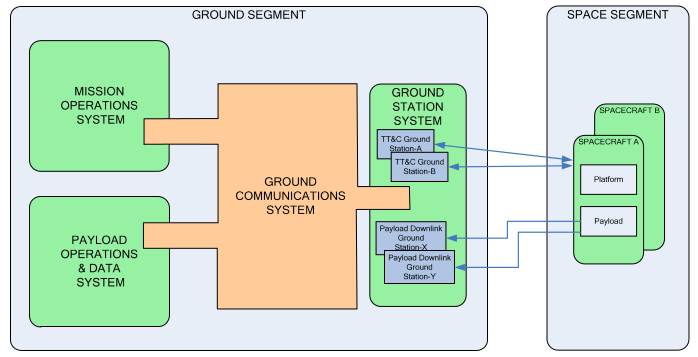
\includegraphics[scale=0.5]{fig/ground_segment_systems}
\caption{Ground Segment Systems (ECSS)}
\label{fig:Ground Segment Systems}
\end{figure}

The \textbf{ground segment} comprises all the \textbf{ground systems} that are used to support the preparation activities leading up to mission operations, the conduct of operations themselves and all post-operational activities. The ground segment as shown in Figure \ref{fig:Ground Segment Systems} typically consists of the following top-level systems:

\begin{itemize}
\item Mission operations system
\item Payload operations and data system
\item Ground station system
\item Ground communications system
\end{itemize}

\subsubsection{Mission Operations System}

The mission operations system typically supports the following:

\begin{itemize}
\item Mission analysis
\item Operations preparation
\item Simulation
\item Mission planning and scheduling
\item Monitoring and control
\item Flight dynamics
\item Onboard software maintenance
\item Data archiving
\item User services
\item Data product delivery
\item Performance analysis and reporting
\item Configuration management (space and ground segment, mission information)
\item System maintenance
\end{itemize}

\subsubsection{Payload Operations and Data System}

The payload operations and data system is used to exploit the mission products and typically supports:

\begin{itemize}
\item Payload operations analysis
\item Payload operations preparation
\item Simulation
\item Payload operations planning and scheduling
\item Payload operations control
\item Payload data processing
\item Payload data archiving
\item User services
\item Data product delivery
\item Performance analysis and reporting
\item Algorithm tuning and development, verification and validation
\item System maintenance
\end{itemize}

\subsubsection{Ground Station System}

The ground station system provides the physical link with the space segment. The following are supported, where applicable:

\begin{itemize}
\item Telemetry reception, storage and distribution
\item Telecommand transmission
\item Tracking, ranging, Doppler and meteorological data acquisition
\item Station monitoring and control
\item Time management
\item Network management and scheduling
\item Data distribution
\item System maintenance
\end{itemize}

\subsubsection{Ground Communications System}

The ground communications system provides the interconnections between systems, such as the connection between ground stations and mission control facilities. The following are supported, where applicable:

\begin{itemize}
\item Data distribution
\item Voice and video communication
\item System maintenance
\end{itemize}

\section{Model-Based System Engineering}

\begin{tabular}{l}
\textit{ECSS-E-TM-10-25 "Engineering design model data exchange (CDF)" \cite{ECSS-E-TM-10-25}} \\
\textit{ECSS-E-TM-10-23 "Space system data repository" \cite{ECSS-E-TM-10-23}} \\
\textit{CCSDS 311.0-M "Reference Architecture for Space Data Systems" \cite{CCSDS-311.0-M}} \\
\textit{"SysML Distilled: A Brief Guide to the Systems Modeling Language" \cite{delligatti2014sysml}}
\end{tabular}

To manage ever more complex systems and their interdependencies, there is a general trend in various engineering domains to move from a \textbf{document-centric} to a \textbf{model-centric} system engineering approach. Both approaches can equally be applied to the system engineering life cycle activities that were presented in the previous sections. The key difference between the two approaches, however, are the nature of the primary artifacts that they produce. 

With the \textbf{document-based} approach, systems engineers manually generate the documents related to system engineering, namely requirements specifications, interface definition documents, design definition documents, and so on. Document-based systems engineers produce these artifacts in the form of a disjoint set of text documents, spreadsheets, diagrams, and presentations (and configuration-manage them in a disjoint set of repositories). The problem is that the task of keeping all those documents in synch and up-to-date, is heavily time-consuming and error prone. Imagine for example just the profane activity of changing the name of an equipments unit; all documents making reference to it will have to be modified as well.

With the \textbf{model-based} system engineering (MBSE) approach, systems engineers perform the same life cycle activities and produce the same set of deliverables. But the deliverables are not the immediate outputs of the life cycle activities; they are not the primary artifacts. With the MBSE approach, the primary artifact of those activities is an integrated, coherent, and consistent system model, created by using a dedicated systems modeling tool. All other artifacts are secondary and automatically generated from the system model using that same modeling tool, which serves as the central repository for the design.

There are three things needed to conduct MBSE, namely:

\begin{itemize}
\item Modeling language
\item Modeling method
\item Modeling tool
\end{itemize}

To create a model, a \textbf{modeling language} is needed first. This is a semiformal language that defines the kinds of elements that can be put in the model, the relationships these elements can have with each other, and the set of notations that can be used to display them visually. The modeling language of choice that has found widespread acceptance is the \textbf{Systems Modeling Language (SysML)}.

While the language specifies the set of rules to determine if a given model is well formed or not, it does not prescribe anything about how to actually construct such a model. It is the chosen \textbf{modeling method} that dictates how and when models shall be created. At present there is no formally established method, but the one described in ECSS-E-TM-10-25 \cite{ECSS-E-TM-10-25} may serve as a good reference.

Not less important is the \textbf{modeling tool}. The tool must comply with the grammar of the modeling language. But different to simple drawing tools that only show diagrams that are drawn following the grammar of the modeling language, the modeling tool must also support the creation of the model itself, which serves as the underlying model for creating such views, and the integrated consistency updates. Although the prospects of MBSE are promising, such tools, in particular those in the open domain, are still not very mature. In addition, the semantics and reference models for use in space system engineering are yet to be formally established.

\clearpage
\section{Deliverables}
\label{sec:Engineering Deliverables}

\subsection{Documents per Review}

\begin{table}[h]
\centering
\begin{tabular}{l c c c c c c c c c}
\toprule
\textbf{Phase} & \textbf{0} & \textbf{A} & \multicolumn{2}{c}{\textbf{B}} & \textbf{C} & \multicolumn{2}{c}{\textbf{D}} & \multicolumn{2}{c}{\textbf{E}} \\
\textbf{Review} & \textbf{MDR} & \textbf{PRR} & \textbf{SRR} & \textbf{PDR} & \textbf{CDR} & \textbf{QR} & \textbf{AR} & \textbf{ORR} & \textbf{FRR} \\
\midrule
Mission description doc.    	& • & • &   &   &   &   &   &   &   \\
\hline
System - TS              	    &(•)&(•)& • &   &   &   &   &   &   \\
\hline
System - I/F TS          	    &   &(•)& • & • &   &   &   &   &   \\
\hline
System engineering plan		    & • & • & • & • & • & • & • &   &   \\
\hline
Verification plan 		        &   & • & • & • & • & • & • &   &   \\
\hline
AIT plan						&   &   &   & • & • & • & • &   &   \\
\hline
Orbital debris mitigation plan	& • & • & • & • & • & • & • & • & • \\
\hline
Coordinate system doc.       	&   & • & • & • & • & • &   &   &   \\
\hline
\hline
Design definition file       	&   & • & • & • & • & • & • &   &   \\
\hline
Function tree               	&   & • & • & • &   &   &   &   &   \\
\hline
Product tree	                &   & • & • & • &   &   &   &   &   \\
\hline
Specification tree           	&   &   & • & • &   &   &   &   &   \\
\hline
Technical budget            	&   & • & • & • & • & • & • &   &   \\
\hline
Element - TS                    &   &(•)& • &   &   &   &   &   &   \\
\hline
Subsystem - TS                  &   &   &(•)& • &   &   &   &   &   \\
\hline
Interface control doc.          &   &   & • & • & • & • & • & • & • \\
\hline
Product user manual  	        &   &   &   &   & • & • & • & • & • \\
\hline
\hline
Design justification file      	&   & • & • & • & • & • & • &   &   \\
\hline
Verification control doc.       &   &(•)&(•)&(•)& • & • & • & • & • \\
\bottomrule
\end{tabular}
\caption{System Engineering Documents required per Review}
\end{table}

(•) = preliminary

\subsection{Documents per Request}

\begin{itemize}
\item Test specification
\item Analysis report
\item Test procedure
\item Test report
\item Review of design report
\item Inspection report
\end{itemize}


\chapterimage{chapter_head_01} % Chapter heading image
\chapter{Mission Operations}
\label{chap:Mission Operations}

\section{Overview}

Mission operations is key element of a space system and plays an essential role in achieving mission success. Mission success is the achievement of the target mission objectives as expressed in terms of the quantity, quality, and availability of delivered mission products and services within a given cost envelope.

\section{Mission Operations Disciplines}

\begin{tabular}{l}
\textit{ECSS-E-ST-70 "Ground systems and operations" \cite{ECSS-E-ST-70}}
\end{tabular}

In order to implement the mission operations process, a number of disciplines are involved. They are described in the following sections.

\subsection{Requirements Analysis and Concept Development}

The input to this process are the requirements captured in the mission description document (Section \ref{sec:Mission Description Document}), the operations domain applicable technical requirements from the technical requirements specification (Section \ref{sec:Technical Requirements Specification}), and the \textbf{launch user manual} (if available). Further, the operability requirements as stated in ECSS-E-ST-70-11 \cite{ECSS-E-ST-70-11} shall be considered.

The \textbf{mission analysis} process shall characterize the constraints and characteristics of the launch, space, and ground segment, and mission-specific constraints. Its main purpose is to take into account the geometrical configuration of the trajectory and orbit of the spacecraft with respect to the ground segment and region of interest for achieving the mission objectives, and to make assessment about the feasibility and constraints. The outcome of the analysis shall be documented in the \textbf{mission analysis report} (Section \ref{sec:Mission Analysis Report}).

The \textbf{operations analysis} process on the other hand is concerned with the assessment of the operational feasibility of the mission. It also defines the onboard mission operations services, together with its corresponding service requests (telecommands) and service reports (telemetry). Further, the interfaces between all entities engaged in mission operations shall be defined in operational interface control documents. The outcome of the operations analysis shall be documented in the \textbf{mission operations concept document} (Section \ref{sec:Mission Operations Concept Document}).

Another important document that contains the schedule for the production and validation of mission operations data and the mission operations team composition, recruitment, and training is the \textbf{operations engineering plan} (Section \ref{sec:Operations Engineering Plan}).

For the validation of operations a number of tests have to be carried out in the operation validation process as presented in Section \ref{sec:Operational Validation}. This information is captured in the \textbf{operational validation plan} (Section \ref{sec:Operational Validation Plan}).

\subsection{Mission Operations Data Production and Validation}

The inputs to \textbf{mission operation data production} process are the documents generated by the requirements analysis and concept development process, together with the \textbf{space segment user manual} (Section \ref{sec:Space Segment User Manual}) and the user manuals of the ground system(s). In addition, the preliminary versions of the \textbf{monitoring and control databases} of space segment and ground segment are needed.

The main objective of this process is to generate the \textbf{mission operations plan} (Section \ref{sec:Mission Operations Plan}) that includes the procedures , rules, timelines, and schedules. It shall also define the operational organization and responsibilities, in particular the decision making process.

The \textbf{operations} procedures (Section \ref{sec:Operations Procedures}) that are part of the mission operations plan (MOP) shall cover the \textbf{nominal and contingency operations} of the space and ground segments.

The \textbf{mission operations data validation process} demonstrates the correctness of the data and its compatibility with the space segment. The major test tool for this is an \textbf{operational simulator}, as a flight representative space segment. The validation is performed invoking all operational procedures and telecommands, all operational modes of the spacecraft (nominal and non-nominal), and all spacecraft redundancies. All results are to be reported.

\subsection{Operations Team Build-Up and Training}

The \textbf{operations organization} is comprised of teams, and typically organized as follows:
 
\begin{itemize}
\item \textbf{Mission control team or flight control team}: Composed of operations manager, operations engineers, analysts, and spacecraft controllers, in charge of the overall control of the mission and of its space segment
\item \textbf{Flight dynamics team}: Providing support to the mission control team for orbit and attitude determination, prediction of orbit and orbital events, preparation of orbital and attitude maneuvers, and calibration of attitude sensors.
\item \textbf{Ground operations team}: In charge of the operations and maintenance of the supporting entities (e.g. ground stations, ground communications network, mission control facility).
\item \textbf{Mission exploitation team}: In charge of planning and processing and distribution of payload data and related ancillary data.
\item \textbf{Ground segment support teams}: Providing support to the ground operations teams.
\item \textbf{Space segment support teams}: Providing support to the mission control team.
\end{itemize}

An \textbf{operations training plan} shall be established that comprises theoretical and practical trainings (e.g. realistic simulations, rehearsals of scenarios and contingency cases). For each team member a \textbf{training record} shall be maintained.

\subsection{Operational Validation}
\label{sec:Operational Validation}

The operational validation (as defined in the operational validation plan (Section \ref{sec:Operational Validation Plan}) is carried out in a realistic operational context (that is, through representative operational scenarios with support of operational simulators), to demonstrate that the ground segment is properly functioning, all mission data is correct, all teams are working well together and are capable of supporting the mission.

The operational validation includes:

\begin{itemize}
\item \textbf{Simulations and rehearsals}: Operational teams execute nominal and contingency operational scenarios from the mission operations plan using the operational simulator in place of the real spacecraft.
\item \textbf{Mission readiness tests}: To validate the readiness of the ground stations to support the mission and to provide training for ground station operators and network staff.
\item \textbf{Data flow tests}: To validate the communications interfaces between ground stations and the control center (telemetry, telecommands, and tracking).
\item \textbf{Tracking campaigns}: Using already flying missions to validate the end-to-end ranging/Doppler system.
\end{itemize}

\subsection{Operations Execution}

Operations execution covers operations of the space segment and the ground segment from launch to disposal. Operations execution can be split into different phases depending on the criticality for the mission as follows:

\begin{itemize}
\item \textbf{Critical phases}: This includes launch and early operations phase (LEOP), commissioning, and orbital insertion.
\item \textbf{Routine phases}: This includes mission exploitation, cruise, and hibernation.
\end{itemize}

\subsubsection{Critical Mission Operations}

The critical mission operations are usually carried out in the presence of a larger team that has all the needed expertise to react upon unexpected behaviour, and the management staff to provide necessary authorization to implement counteractions. Therefore, such operations are typically conducted in a larger \textbf{multi-mission control room}.

\subsubsection{Routine Mission Operations}

The routine mission operations form the largest part of the operational activities. Therefore they are typically conducted from a smaller, \textbf{dedicated control room}, with the minimal needed infrastructure (but including redundancies, of course). Also, there is the tendency to automate most of the activities in this phase, in order to reduce manpower and therefore costs.

The following activities are typically executed during routine mission operations:

\begin{itemize}
\item \textbf{Mission planning}: Mission planning is the generic term referring to the process of identifying and organizing the activities required to achieve the mission objectives. It is an iterative process and generally overlaps with scheduling. In particular it comprises the following:

	\begin{itemize}
	\item \textbf{Science/objective planning}: The user (e.g. scientist, customer) inputs requests on operations (science observations at defined times, image taking at defined orbit position and attitude, etc.). This is then translated into configuration requirements for payload and platform.

	\item \textbf{Maneuver operations planning}: Flight dynamics provides times at which attitude/orbit maneuvers shall be executed, for purpose of orbit/attitude keeping or in respect to science/objective requirements.

	\item \textbf{Special operations planning}: All other necessary planning activities, such as planning for eclipses, hibernation, cruise phase, in-orbit tests, etc.
	\end{itemize}

\item \textbf{Preparation of operations schedules}: Scheduling is the generic term for the process of determining the sequential order of activities, assigning planned duration and determining the start and finish dates of each activity. Again, scheduling is an interactive process as well and has the planning activities as a prerequisite. Scheduling comprises for example:

	\begin{itemize}
	\item \textbf{Onboard schedules}: Define when and for how long elements of the spacecraft are active or in a certain mode. Typical output of this is a timeline of commands to be uplinked to the spacecraft and executed at specified times in the future. 
	\item \textbf{Pass schedules}: Specify the times during which a ground station is tracking a spacecraft. 
	\item \textbf{Shift schedules}: Specify for example when ground stations and control rooms are staffed.
	\end{itemize}
	
\item \textbf{Execution and verification of operations schedules}: This activity covers the uplink of commands and ensuring that those are carried out accordingly.

\item \textbf{Health monitoring}: Comprises of reception and checking of telemetry (for example, checking whether parameters are within defined limits, and checking the downloaded onboard logs).  

\item \textbf{Preservation of mission history data}: Comprises the long-term archival of monitoring and control data from space and ground segment for purpose of performance evaluation, anomaly investigations, etc.

\item \textbf{Mission products processing}: Comprises the processing of mission data, its archiving, and distribution to end users (possibly together with ancillary data).

\item \textbf{Anomaly handling}: At occurrence of anomalies that are not yet handled by contingency procedures, an anomaly review board meeting is called for to determine corrective actions, which then shall be elaborated into a new procedure that has to be validated, approved, and implemented.

\end{itemize}

\subsubsection{Operations Reporting} 
\label{sec:Operations Reporting}

The \textbf{nominal operations reports} are issued on periodic basis. Those reports state the operations and maintenance carried out, and anomalies encountered, during the reporting period. The periodicity of such reports depend on the mission phase. Typically such reports are issued daily during critical phases, and weekly during routine phases.

In addition, \textbf{summary reports} are issued for critical operations periods, such as LEOP, commissioning, and other critical operations. Other non-periodic reports include \textbf{performance reports} on space and ground segment, and \textbf{anomaly reports}. Anomaly reports are used to document a departure from expected performance during operations, for both the ground and space segment (Section \ref{sec:Operations Anomaly Report}).

Other reports are prepared when required or regarded as beneficial to future missions, for example, lessons learned, spacecraft in-orbit performance, and so on.

\subsection{Space Segment Disposal Operations}

The space segment disposal activities comprise the preparation and execution of spacecraft disposal, dominantly through atmospheric re-entry and subsequent burn-up. It shall comply with any space debris mitigation requirements that are imposed internally or externally (such as via international regulations or the launch authority). To achieve the disposal, corrective orbit maneuvers may be needed.

\section{Deliverables}
\label{sec:Mission Operations Deliverables}

\subsection{Documents per Review}

\begin{table}[h]
\centering
\begin{tabular}{l c c c c c c c c c}
\toprule
\textbf{Phase} & \textbf{0} & \textbf{A} & \multicolumn{2}{c}{\textbf{B}} & \textbf{C} & \multicolumn{2}{c}{\textbf{D}} & \multicolumn{2}{c}{\textbf{E}} \\
\textbf{Review} & \textbf{MDR} & \textbf{PRR} & \textbf{SRR} & \textbf{PDR} & \textbf{CDR} & \textbf{QR} & \textbf{AR} & \textbf{ORR} & \textbf{FRR} \\
\midrule
Mission analysis report     	&   &(•)& • & • & • & • &   &   &   \\
\hline
Mission operations concept doc.	&   &(•)& • & • &   &   &   &   &   \\
\hline
Operations engineering plan    	&   &   &   &(•)& • &   &   &   &   \\
\hline
Operational validation plan	    &   &   &   &   &   &   &   & • &   \\
\hline
Operations training plan        &   &   &   &   &   &   &   & • &   \\
\hline
Mission operation plan			&   &   &   &   &   &   &   & • &   \\
\hline
Operational validation reports  &   &   &   &   &   &   &   & • & • \\
\bottomrule
\end{tabular}
\caption{System Engineering Documents required per Review}
\end{table}

(•) = preliminary

\subsection{Documents per Request}

\begin{itemize}
\item LEOP reports
\item Commissioning reports
\item Performance reports
\item Routine operations reports
\item Operations anomaly reports
\item Mission reports
\item Disposal operations reports
\end{itemize}


\part{Systems}

\chapterimage{chapter_head_01} % Chapter heading image
\chapter{Space System}

\section{Overview}

The highest level system of a space mission is termed the space system. Examples are: the Global Positioning System (GPS), the European Data Relay System (EDRS), or Disaster Monitoring Constellation for International Imaging (DMCii), to name a few.

The further breakdown of a typical space system is provided provided in ECSS-S-ST-00-01 \cite{ECSS-S-ST-00-01} as follows. First, the space system is functionally categorized into three segments: space segment, ground segment, and launch segment. Each segment is further decomposed as shown exemplary for the space segment:

\begin{itemize}
\item space segment (functional)
\item space segment system (functional)
\item space segment element 
\item space segment subsystem (functional)
\item space segment equipment/unit
\item components/parts
\end{itemize}

Functional elements are logical grouping of physical elements. Figure \ref{fig:Space System Breakdown Schema} visualizes the ECSS approach for achieving a breakdown of the system.

\begin{figure}[h]
\centering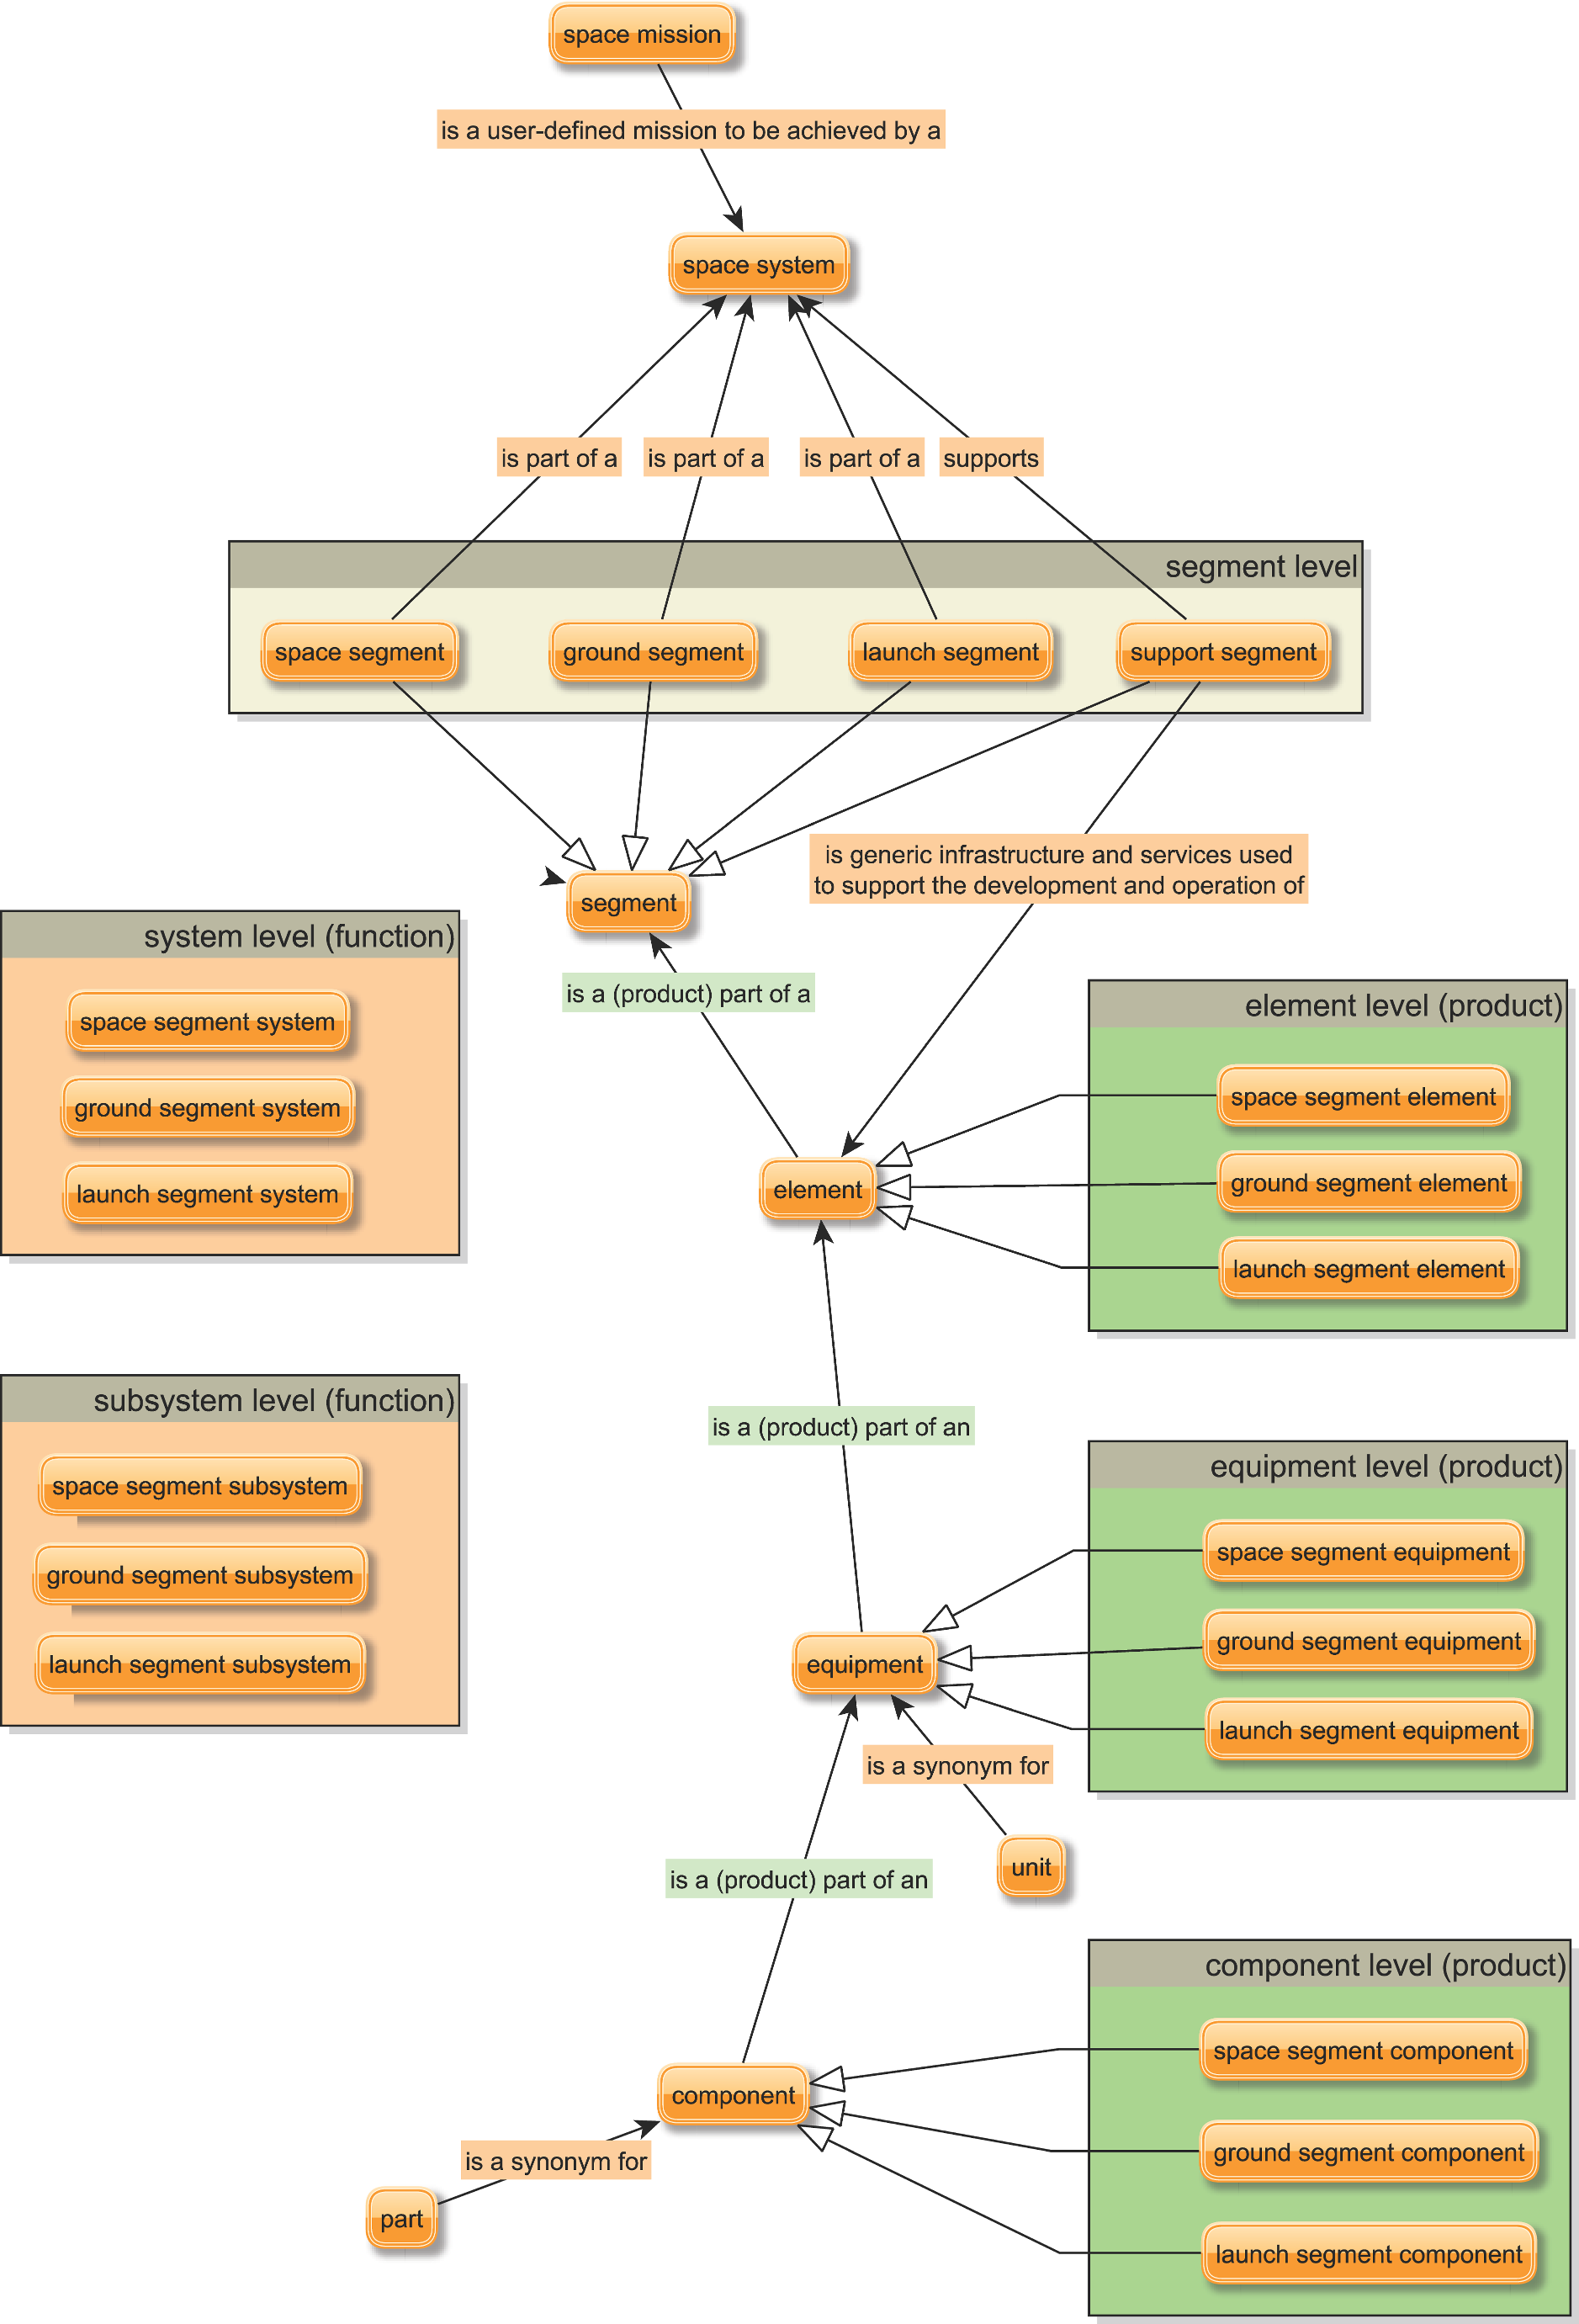
\includegraphics[width=1.0\linewidth]{fig/system_decomposition}
\caption{Space System Breakdown Schema (copyright ECSS)}
\label{fig:Space System Breakdown Schema}
\end{figure}

\section{Formats}

There are almost no standards that are applicable to the entire space system as such. Of those that are, they are concerned with formats of data to be used across the segment boundaries.

\subsection{Time}

\begin{tabular}{l}
\textit{CCSDS-301.0-B "Time Code Formats" \cite{CCSDS-301.0-B}} \\
\end{tabular}

Time codes are digital representations of time information. Four time codes are available: one unsegmented and three segmented time codes. All use the international standard second as the fundamental unit of time. An unsegmented time code is a pure binary count of time units and fractional time units from a starting time called the epoch. A segmented time code is one in which the count of time units and fractional time units is accumulated in two or more cascaded counters which count modulo of various bases and start from the epoch. 

The \textbf{CCSDS unsegmented time code} (CUC) consists of a number of contiguous octets representing an integrated  number of the basic time unit from a defined epoch along with an optional integer number of octets representing the elapsed binary fraction of the basic time unit. The time code increases monotonically without reversion. The CCSDS-Recommended epoch is that of 1958 January 1 and the recommended time unit is the second, using TAI as reference time scale. This time code is not UTC-based and leap-second corrections do not apply. 

The \textbf{CCSDS day segmented time code} (CDS) consists of a 16 or 24 bit counter for the day from epoch, a 32 bit counter for the milliseconds of the day and optionally a 16/32 bit counter for the submilliseconds. The CCSDS recommended day segment is a continuous counter of days from 1958 January 1 starting with 0. Since this code is UTC-based, the leap second correction must be made. 

The \textbf{CCSDS calendar segmented time code} (CCS) is defined in month of year / day of month format, or as day of year format. Both CCS time code variations are UTC-based. The leap second correction must be made.

The \textbf{CCSDS ASCII segmented  time code} is composed of a variable number of ASCII 
characters and defined in month of year / day of month format, or as day of year format. Both ASCII time code variations are UTC-based and leap second corrections must be made. The time represented is intended to match civil time usage.  Therefore, the epoch is taken to be the usual Gregorian calendar epoch of 1 AD, and the time is that of the prime meridian. The format is:

ASCII time code A: YYYY-MM-DDThh:mm:ss.d$\rightarrow$dZ (e.g. 1988-01-18T17:20:43.123456Z)
ASCII time code B: YYYY-DDDThh:mm:ss.d$\rightarrow$dZ (e.g. 1988-018T17:20:43.123456Z)

where:

\begin{tabular}{l l}
DDD & is day of year, \\
T & is the calendar-time separator, \\
d$\rightarrow$d & is decimal fraction of second, and \\
Z & is the optional time code terminator.
\end{tabular}
 
\subsection{Identifiers}

\begin{tabular}{l}
\textit{CCSDS-320.0-B "CCSDS Global Spacecraft Identification Field..." \cite{CCSDS-320.0-B}} \\
\end{tabular}

The CCSDS SCID (spacecraft identifier) is a 10-bit number used in telecommand and telemetry frames and serves as a mechanism for the identification of a simple spacecraft having only one logical space-ground link; or an association between space-based and ground-based application processes with complex spacecraft having more than one logical space-ground link.

CCSDS has established the Space Assigned Numbers Authority (SANA) \cite{sanaregistry.org}, which coordinates the issuing of SCID to different spacecraft. It has the objective to eliminate the possibility that data from any given CCSDS-compatible vehicle will be falsely interpreted as being from another CCSDS-compatible vehicle or commands sent to a CCSDS-compatible vehicle will be received and acted upon by application processes for which they were not intended.


\chapterimage{chapter_head_01} % Chapter heading image
\chapter{Space Segment}

\section{Overview}

One or more spacecraft make up the space segment. A spacecraft is composed of one or more payloads, and the spacecraft bus, also called platform. The platform is in turn composed of a number of subsystems that each provide some functional aspect for supporting the payload operations.

\section{Payload}

The payload system provides the functionality to fulfill the specific mission objectives. For earth observation mission the payloads may be optical cameras or other remote sensing instruments. For communications mission the payload may be a transponder. For science missions the payload may be a certain type of novel instrument. With such a variety of mission objectives the standardization of payloads on system level is an unrealistic approach. On the other hand, what can be standardized to some extended is the interfaces to it, and possibly some of its onboard data processing.

\subsection{Data Compression}

\subsubsection{Lossless Data Compression}

\begin{tabular}{l}
\textit{CCSDS-121.0-B "Lossless Data Compression" \cite{CCSDS-120.0-G}} \\
\textit{CCSDS-120.0-G "Lossless Data Compression" \cite{CCSDS-121.0-B}}
\end{tabular}

The lossless source coding technique preserves source data accuracy and removes redundancy in the data source. This technique is particularly useful when data integrity cannot be compromised. The described lossless source coder consists of two separate functional parts: the preprocessor and the adaptive entropy coder. 

The role of the \textbf{preprocessor} is to transform the data into samples that can be more efficiently compressed by the entropy encoder. It applies a reversible function to input data samples to produce the lowest entropy, which is a measure of the smallest average number of bits that can be used to represent each sample. In general a preprocessor that removes correlation between samples in the input data block will improve the performance of the entropy coder. The \textbf{adaptive entropy coder} uses variable-length codes and compresses data by assigning shorter codewords to symbols that are expected to occur with higher frequency. By using several different codes and transmitting the code identifier, the algorithm can adapt to many sources from low entropy (more compressible) to high entropy (less compressible).

\begin{tabular}{l}
\textit{CCSDS-123.0-B "Lossless Multispectral and Hyperspectral Image Compression" \cite{CCSDS-123.0-B}}
\end{tabular}

The described compressor is applicable to three-dimensional arrays of integer sample values (as obtained from multispectral and hyperspectral imagers and sounders). It consists of two functional parts: a predictor and an encoder. The \textbf{predictor} has as input the original image data and predicts the value of each image sample based on the values of nearby samples in a small three-dimensional neighbourhood. These mapped predictions make up the predictor output. The \textbf{encoder} then works similar as the adaptive entropy encoder presented above, using statistical data that is updated after each sample is encoded.

\subsubsection{Lossless and Lossy Image Data Compression}

\begin{tabular}{l}
\textit{CCSDS-122.0-B "Image Data Compression" \cite{CCSDS-122.0-B}} \\
\textit{CCSDS-120.1-G "Image Data Compression" \cite{CCSDS-120.1-G}}
\end{tabular}

Several lossless and lossy image compression algorithms are widely used, such as JPEG2000 and JPEG-LS. This standard however describes a fast and less complex algorithm that can be applied to greyscale images with integer-valued pixels with a bit depth of 16 bits. It consists of two functional parts: a discrete wavelet transform and a bit-plane encoder. The \textbf{discrete wavelet transform} performs low-pass and high-pass filtering along first horizontal and then vertical direction, resulting in four subband data arrays, each half as wide and half as tall as the original image array. This step is repeated two more time, each time with the obtained left upper subband data array as input. This produces a total of 10 subbands. The \textbf{bit-plane encoder} then processes 64 wavelet coefficients, which are made up from the 16 equally sized blocks of the most upper left subband (termd the DC coefficients) and their mapping to the other subbands.

\subsubsection{Digital Motion Imagery}

\begin{tabular}{l}
\textit{CCSDS-766.1-B "Digital Motion Imagery" \cite{CCSDS-766.1-B}} \\
\textit{CCSDS-706.1-G "Motion Imagery and Applications" \cite{CCSDS-706.1-G}}
\end{tabular}

This standard categories different video applications and relates to it appropriate video resolutions and frame rates. It specifies the commonly used MPEG-4 Part 10 (H.264) as the encoding format intended for real-time applications where live, or nearly live, video needs to be monitored at a ground location during an event or experiment. Further, JPEG2000 is intended for requirements for higher quality or where each individual frame needs to be maintained intact. 

\section{Platform}

\subsection{Mechanical}

\subsubsection{Structure}

\begin{tabular}{l}
\textit{"CubeSat Design Specification" \cite{cubesat_design_specification}}
\end{tabular}

The main purpose of the CubeSat design specification (CDS) is to ensure that CubeSats can fit inside a deployment system, of which California Polytechnic State University's P-POD (Poly Picosatelite Orbital Deployer) sets the standard, and to ensure that the CubeSat does not pose a threat to neighboring payloads. While the specification's main focus is on the definition of the mechanical outline of the primary structure and its geometrical properties, it also includes requirements on the material to be used and its surface finish. The original CDS introduced the cubic shaped 10x10x10 cm$^{3}$ single unit (1U) CubeSat design (as shown in Figure \ref{fig:1U CubeSat Design Specification Drawing}), however now the specification also includes definitions for multiples thereof (e.g. 1.5U, 2U, 3U, 3U+).

\begin{figure}[h]
\centering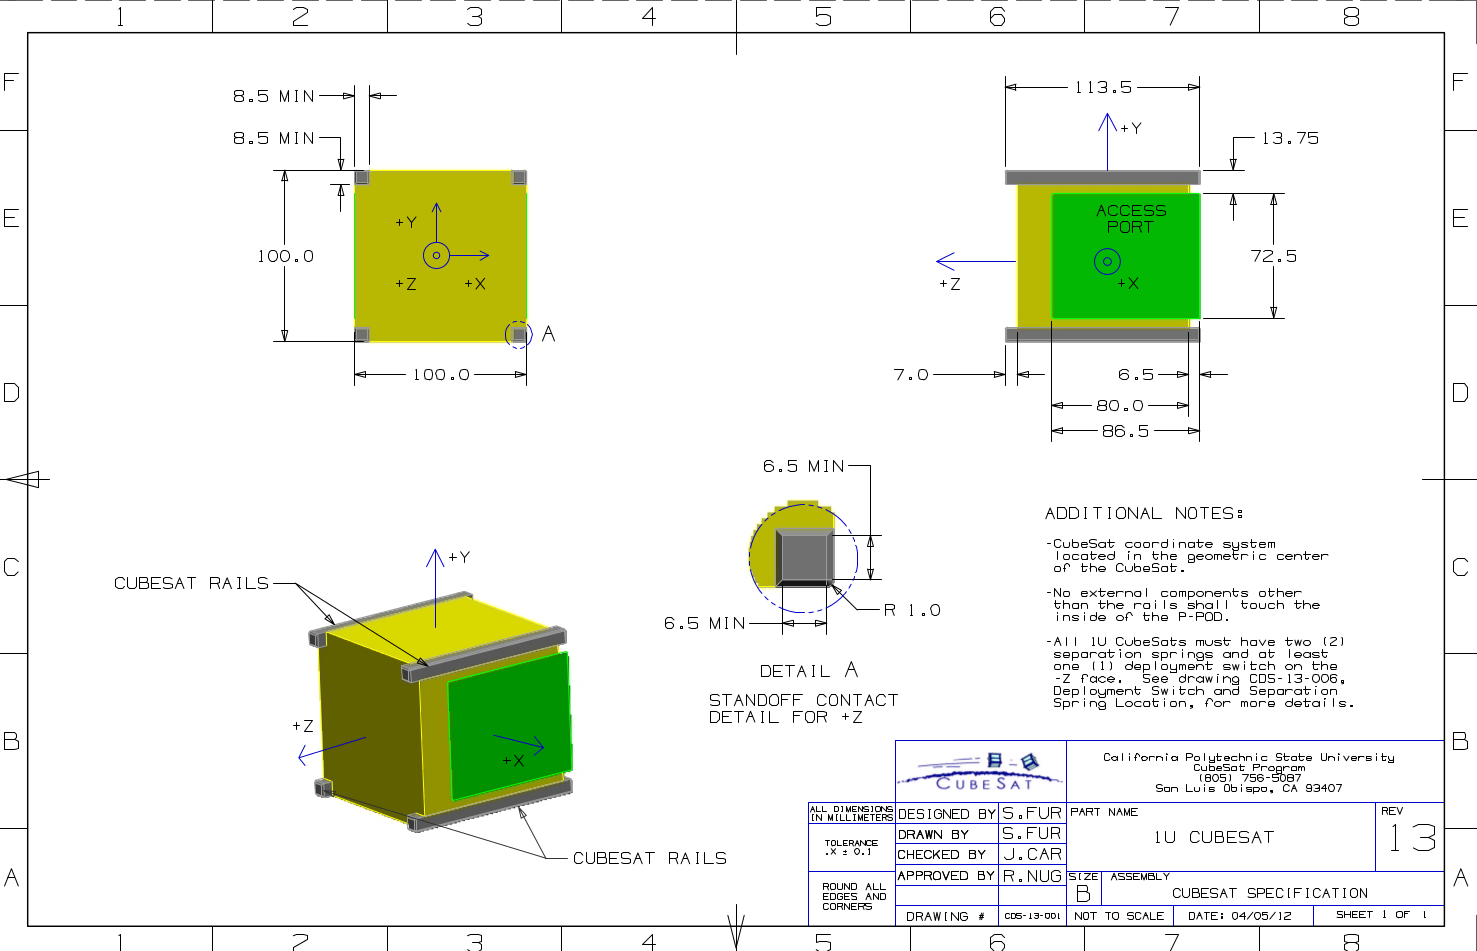
\includegraphics[scale=0.25]{fig/1u_cubesat_design_specification_drawing}
\caption{1U CubeSat Design Specification Drawing}
\label{fig:1U CubeSat Design Specification Drawing}
\end{figure}

\subsubsection{Mechanisms}

\begin{tabular}{l}
\textit{"CubeSat Design Specification" \cite{cubesat_design_specification}}
\end{tabular}

The design of mechanisms is very much mission specific. Deployments from CubeSats, such as booms or wires, have not reached a sufficient maturity that even a best practises could be derived. The exception to this is the definition of two mechanisms that part of the CubeSat specification: separation springs and deployment switches. Usually several CubeSats are launched inside a single deployer. The purpose of the \textbf{separation springs} is then to ensure adequate separation of CubeSats when ejected from the deployer. They are for obvious reasons not required on CubeSats that are contained in equally sized deployment containers. The purpose of the \textbf{deployment switches} is to completely power-off the CubeSat during launch while inside the deployer. The two separation springs and two deployment switches shall be integrated at the four rails on the -Z facing end and shall be diagonal to each other.  

\subsection{Electrical}

\subsubsection{Power Distribution Switches}

\begin{tabular}{l}
\textit{ECSS-E-ST-20-20 "Electrical design and interface requirements for power supply" \cite{ECSS-E-ST-20-20}} \\
\textit{ECSS-E-HB-20-20 "Guidelines for electrical design and interface requirements for power supply" \cite{ECSS-E-HB-20-20}} \\
\end{tabular}

Two types of power distribution switches are available. The \textbf{latching current limiter} (LCL) is a switchable and latching protection between a power source and the load, causing a trip off after having achieved at its outputs and over-current limitation for a defined trip-off time (Figure \ref{fig:LCL Generic Block Diagram}). In case of a load malfunction implying an overload, they enter current limitation mode for the given trip off time duration, and then switch off. LCLs can be externally commanded into ON or OFF mode.

The \textbf{retriggerable latching current limiter} (RLCL) is an LCL that automatically attempts to switch ON when powered or after a retrigger interval when a trip off event occurred. RLCLs are normally used to supply essential spacecraft loads (for example decoders, receivers, and reconfiguration modules) and as such they are supposed to provide continuously power to the load after start up. They react similar to a load malfunction, namely to limit current and then switch off. But they will attempt a re-start automatically after a defined time duration.

\begin{figure}[h]
\centering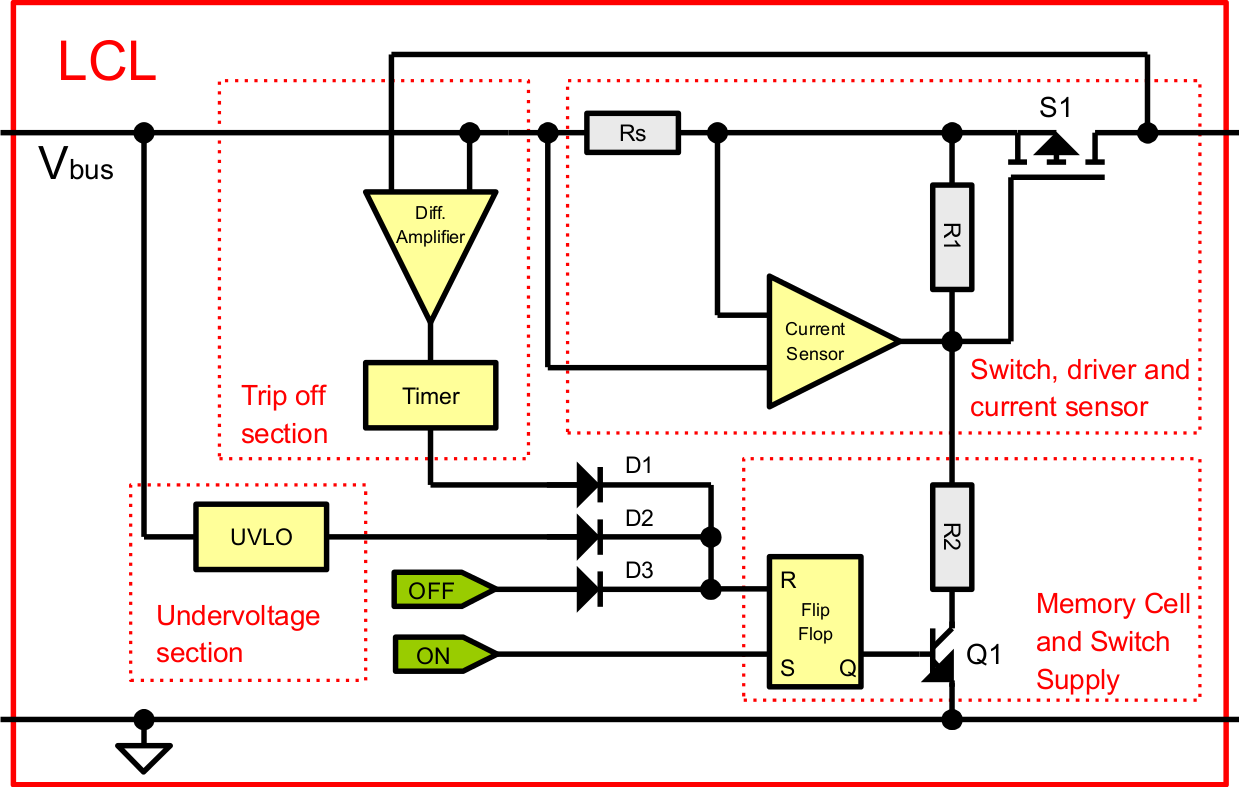
\includegraphics[scale=0.2]{fig/lcl_generic_block_diagram}
\caption{LCL Generic Block Diagram}
\label{fig:LCL Generic Block Diagram}
\end{figure}

\subsubsection{Discrete Interfaces}

\begin{tabular}{l}
\textit{ECSS-E-ST-50-14 "Spacecraft discrete interfaces" \cite{ECSS-E-ST-50-14}} \\
\end{tabular}

Discrete interfaces are used typically for sensor acquisition and actuator control. These interfaces can be broadly categorized into the following types: analog, bi-level digital, pulse commands, and serial digital interfaces. For units that are to be used in redundancy, the driver and receiver interfaces are to be cross-strapped as shown in Figure \ref{fig:General Scheme of Cross-Strapping}.

\begin{figure}[h]
\centering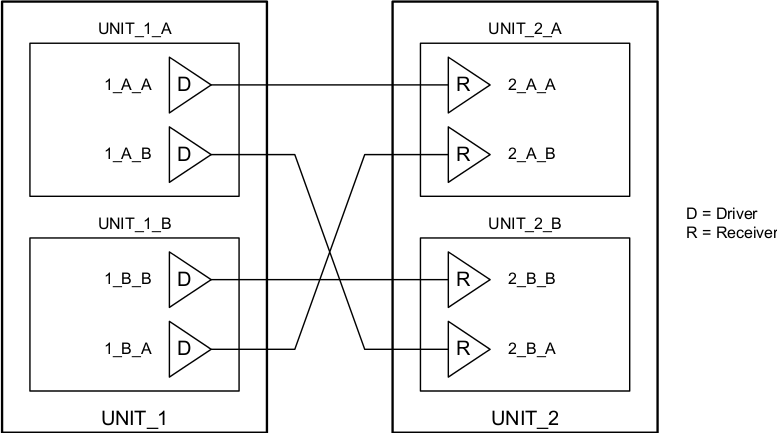
\includegraphics[scale=0.4]{fig/general_scheme_of_cross_strapping}
\caption{General Scheme of Cross-Strapping}
\label{fig:General Scheme of Cross-Strapping}
\end{figure}

The \textbf{analog signal interfaces} are used for direct connection to a device which produces a continuous variable analog voltage to indicate the value of the parameter being measured. Usually, the analog voltage produced by the sensor or a peripheral element is converted into a digital value within the element to which it is connected. The basic application scenario is a differential voltage range from 0 to 5 V with a signal bandwidth of up to 1 Hz (i.e. a slowly changing, quasi-static signal) and a conversion resolution of 12 bits.

A special case of analog signals are \textbf{temperature sensors} (thermistors). These are resistors that change resistance with temperature, either with the temperature gradient (positive temperature coefficient, PTC) or opposite (NTC). Figure \ref{fig:Temperature Sensor Interface Arrangement} shows a typical temperature sensor interface arrangement.

\begin{figure}[h]
\centering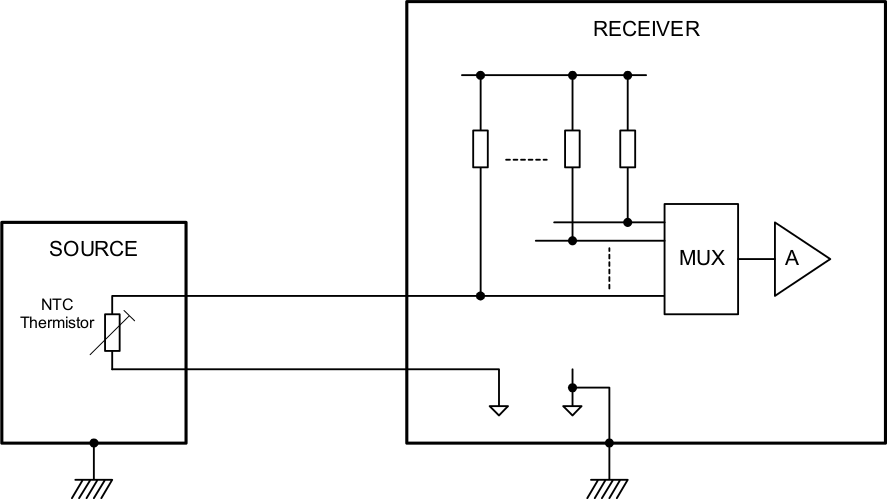
\includegraphics[scale=0.3]{fig/temperature_sensor_interface_arrangement}
\caption{Temperature Sensor Interface Arrangement}
\label{fig:Temperature Sensor Interface Arrangement}
\end{figure}

The \textbf{digital signal interfaces} are used for signals that take only two values, high or low, indicated by the signal voltage. Typically the low voltage ranges from 0 to 0.9 V and high voltage from 2.0 to 5.5 V for a 5 V interface. The signal sources are high impedance, meaning that they carry only a small current in the order of micro- or milliampere. Note that a number of such interfaces can be arranged in parallel to form an arrangement for transmission of larger data words and associated clock and read/write control capabilities.

The \textbf{pulsed command interfaces} on the other hand are intended for load driving interfaces and, for example, can be used to switch relays or similar loads. They provide high current capabilities in the order of up to 1 Ampere. A typical high power commanding interface arrangement is shown in Figure \ref{fig:High Power Commanding Interface Arrangement}.

\begin{figure}[h]
\centering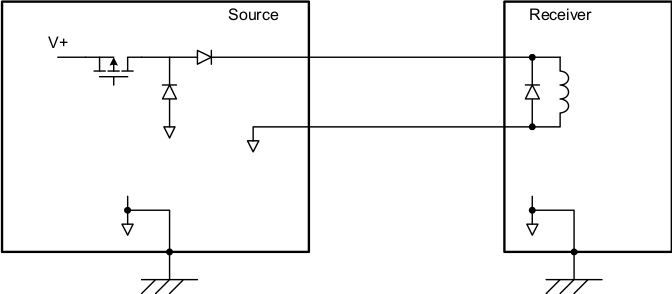
\includegraphics[scale=0.3]{fig/high_power_commanding_interface_arrangement}
\caption{High Power Commanding Interface Arrangement}
\label{fig:High Power Commanding Interface Arrangement}
\end{figure}
 
The \textbf{serial digital interfaces} for point-to-point communication are used to exchange digital data words between core and peripheral elements. Typically universal asynchronous receiver/transmitter (UART) are used for that. It takes bytes of data and transmits the individual bits in a sequential fashion. At the destination, a second UART re-assembles the bits into complete bytes. The UART usually does not directly generate or receive the external signals used between different items of equipment. Separate interface devices are used to convert the logic level signals of the UART to and from the external signaling levels. External signals may be of many different forms. Common microcontrollers support the RS-232 specification that is also known as the serial port on computers. The RS-422 is similar to it but provides for differential signal levels and hence requires two lines per transmit/receive signal. In both cases an intermediate circuit element is needed to convert from CMOS/TTL levels coming from the microcontroller to the larger voltage levels required by the RS-232/RS-422 specification.
 
\subsubsection{Data Bus}

\begin{tabular}{l}
\textit{ECSS-E-ST-50-15 "CANbus extension protocol" \cite{ECSS-E-ST-50-15}} \\
\end{tabular}

Data buses are used for spacecraft on-board communications and control. Typically the data rates are moderate, as they are intended to route telecommands and telemetry, but usually are not indented for streaming science or other high-volume data. The main objective of the data bus is to be highly reliable.

The CAN (Controller Area Network) bus has been successfully used in automotive and critical control industry for more than three decades. The ECSS-CAN standard specifies the requirements for the use of CAN data bus in spacecraft onboard applications. They extend the CAN network specification to cover aspects of the physical and data link layer related to the particular needs of spacecraft data handling systems. 

CAN is by itself a multi-master network, so each node may send messages at any time. Collisions get resolved by message priority. For this to work, each CAN message identifiers used in a network must be unique. A CAN network is composed of two or more nodes. Each of these nodes (see Figure \ref{fig:CAN Bus Node}) include a central processing unit (such as microcontroller), a CAN controller (often integrated in microcontroller), and a CAN transceiver. 

\begin{figure}[h]
\centering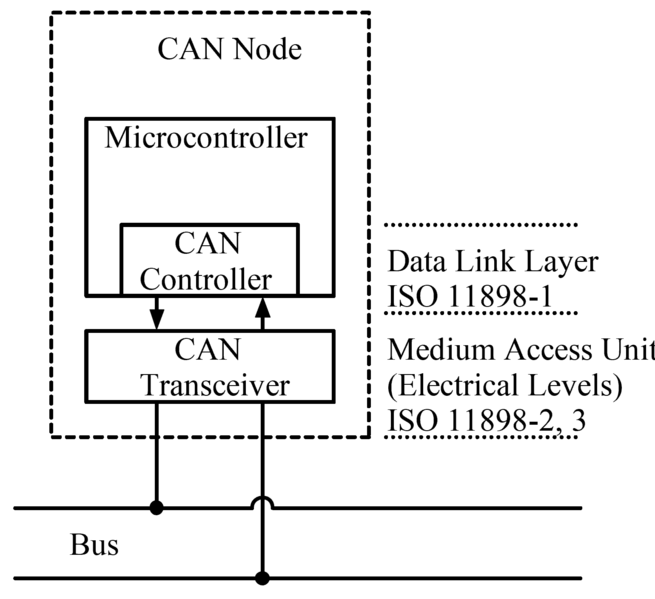
\includegraphics[scale=0.3]{fig/can_bus_node}
\caption{CAN Bus Node}
\label{fig:CAN Bus Node}
\end{figure}

CAN may be implemented on different physical transmission media like twisted pair, power lines, optical and others. A CAN transceiver is used to connect the CAN controller and the physical medium. The transceiver takes the TTL (or CMOS) signal from the controller’s transmit pin and converts it to a differential signal between the two wires of the network cable. In return, differential signals on the two wires of the network cable are converted back into TTL/CMOS level and fed back to the controller’s receive pin.

The data link layer represents the kernel of the CAN protocol. It is responsible for bit timing and synchronization, message framing, arbitration, acknowledgement, error detection and signaling, and fault confinement.

The CAN standard does not include tasks of application layer protocols, such
as flow control, device addressing, and transportation of large data blocks. Many
implementations of higher layer protocols were created to address those issues. The CANopen specification is one of the most widespread protocol stack for industrial applications and has been adopted for the ECSS-CAN bus extension protocol as optional for use as an application layer protocol. 

CANopen is a communication protocol and device profile specification for embedded systems used in automation. In terms of the OSI (Open Systems Interconnection) model, CANopen implements the layers above and including the network layer. The CANopen standard consists of an addressing scheme, several small communication protocols and an application layer defined by a device profile (see Figure \ref{fig:CANopen Device Model}). The communication protocols have support for network management, device monitoring and communication between nodes, including a simple transport layer for message segmentation/desegmentation.

\begin{figure}[h]
\centering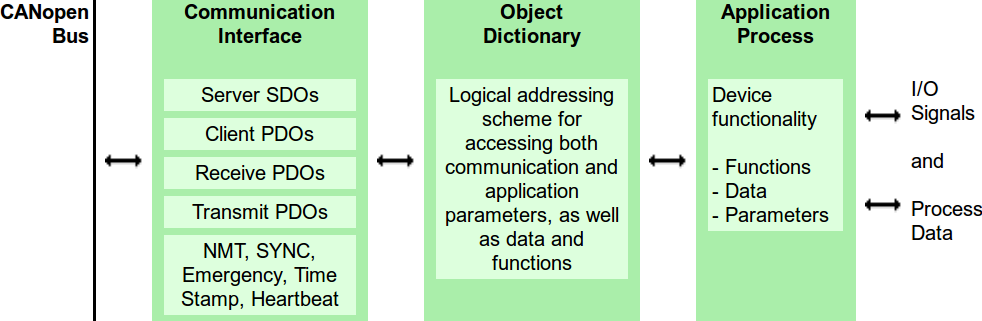
\includegraphics[scale=0.4]{fig/canopen_device_model}
\caption{CANopen Device Model}
\label{fig:CANopen Device Model}
\end{figure}


\subsection{Attitude and Orbit Control}

\subsubsection{Sensors}

\begin{tabular}{l}
\textit{ECSS-E-ST-60-20 "Stars sensors terminology and performance specification" \cite{ECSS-E-ST-60-20}} \\
\end{tabular}

This standard defines the terminology and specification definitions for the performance of star trackers (in particular, autonomous star trackers). It focuses on the specific issues involved in the specification of performances of star trackers and is intended to be used as a structured set of systematic provisions. The standard defines and normalizes terms used in star sensor performance specifications, as well as some performance assessment conditions:

\begin{itemize}
\item Sensor components
\item Sensor capabilities
\item Sensor types
\item Sensor reference frames
\item Sensor metrics
\end{itemize}

\begin{tabular}{l}
\textit{ECSS-E-ST-60-21 "Gyro terminology and performance specification" \cite{ECSS-E-ST-60-21}} \\
\end{tabular}

Similar to the star tracker specification, this standard defines the terminology and specifications for the functions and performance of gyros used on spacecraft. This includes effects of gyro warm-up, bias stability, alignments, and so on. 


\subsection{Space Link}
\label{sec:Space Link}

\begin{tabular}{l}
\textit{ECSS-E-ST-50 "Communications" \cite{ECSS-E-ST-50}} \\
\textit{ECSS-E-HB-50 "Communications guidelines" \cite{ECSS-E-HB-50}} \\
\textit{CCSDS-130.0-G "Overview of Space Communications Protocols" \cite{CCSDS-130.0-G}}
\end{tabular}

The purpose of space link communication is the provision of end-to-end communication services to and from spacecraft. These links are generally between spacecraft and ground, but also include spacecraft-to-spacecraft links, as well as links between spacecraft and landed elements such as rovers. 

\begin{figure}[h]
\centering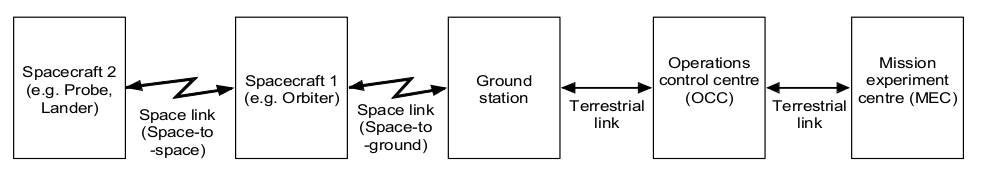
\includegraphics[scale=0.4]{fig/example_configuration_of_a_space_communication_system}
\caption{Example Configuration of a Space Communication System}
\label{fig:Example Configuration of a Space Communication System}
\end{figure}

A communications protocol is usually associated with one of the seven layers defined in the OSI Basic Reference Model. As in most terrestrial networks, protocols of the Session and Presentation Layers of the OSI model are rarely used over space links. Therefore the space link communications protocols are defined for the following five layers:

\begin{itemize}
\item Physical layer
\item Data Link layer
\item Network layer
\item Transport layer
\item Application layer
\end{itemize}

Figure \ref{fig:Space Communications Protocols Reference Model} shows the available space communications protocols and their associated layer.

\begin{figure}[h]
\centering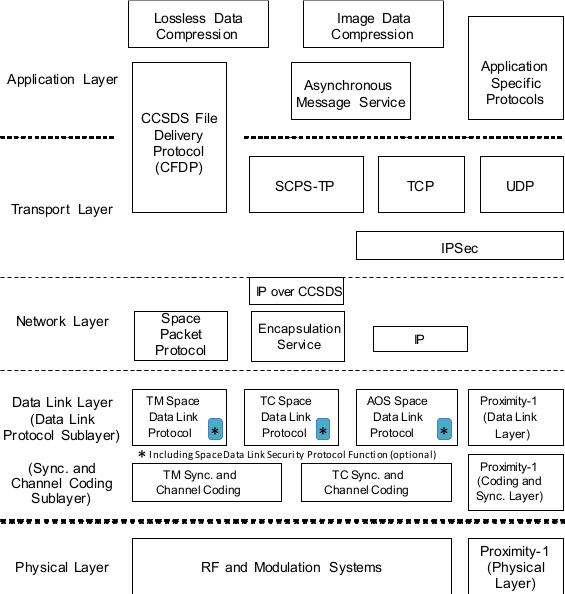
\includegraphics[scale=0.7]{fig/space_communications_protocols_reference_model}
\caption{Space Communications Protocols Reference Model}
\label{fig:Space Communications Protocols Reference Model}
\end{figure}

\subsubsection{Physical Layer}

\begin{tabular}{l}
\textit{CCSDS-401.0-B "Overview of Space Communications Protocols" \cite{CCSDS-401.0-B}} \\
\textit{CCSDS-413.0-G "Bandwidth-Efficient Modulations" \cite{CCSDS-413.0-G}} \\
\textit{ECSS-E-ST-50-05 "Space engineering - Radio frequency and modulation" \cite{ECSS-E-ST-50-05}}
\end{tabular}

The physical layer specification covers the characteristics of the radio frequency and modulation systems. It specifies the properties of the RF signals, namely the frequency stability, polarization, bandwidth occupations, and emissions, as well as the signal modulation (categorized into two categories: with residual carrier and with suppressed carrier). Further, link acquisition procedures and link budget calculations are defined.

\subsubsection{Data Link Layer}

\begin{tabular}{l}
\textit{CCSDS-130.2-G "Space Data Link Protocols--Summary of Concept and Rationale" \cite{CCSDS-130.2-G}}
\end{tabular}

The protocol data units used by the data link layer are called \textbf{transfer frames}. Each transfer frame consists of a header which provides protocol information and a data field within which \textbf{service data units} (SDU) are carried.

The sending of \textbf{telemetry} from a spacecraft to a ground station (the \textbf{return link}) uses fixed-length \textbf{telemetry transfer frames} (TMTF) to facilitate robust synchronization procedures over a noisy link. Their length is fixed on a particular physical channel and must be known to the receiving end before the actual reception occurs.

The sending of \textbf{telecommands} from ground to space (the \textbf{forward link}) uses variable-length \textbf{telecommand transfer frames} (TCTF) to facilitate reception of short messages with a short delay. The length of the frame is contained in its header. In order to notify the sender of TCTFs about the status of acceptance of TCTFs at the receiving end, another data unit called the communications link control word (CLCW) is embedded in the return link (i.e. in the telemetry). 

The mechanism used by the data link layer protocol for transferring data with different quality of service (QoS) requirements (mostly priority and latency) is the use of \textbf{virtual channels} (VC). The virtual channel concept allows one physical channel to be divided into multiple separate logical data channels, each identified by a virtual channel identifier (VCID). Each transfer frame transferred over a physical channel belongs to one of the virtual channels of the physical channel (see Figure \ref{fig:Virtual Channels}).

\begin{figure}[h]
\centering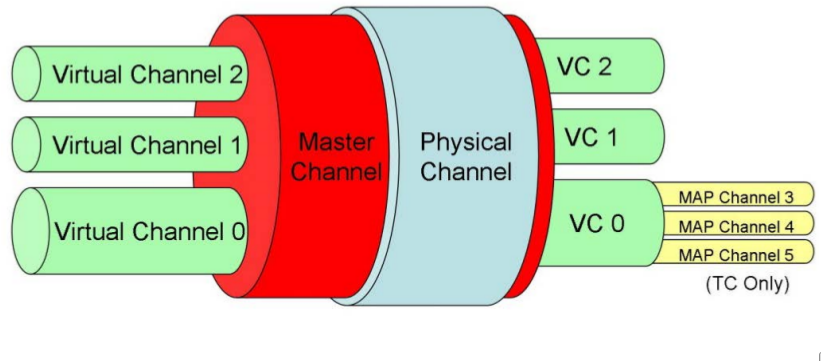
\includegraphics[scale=0.4]{fig/virtual_channels}
\caption{Virtual Channels}
\label{fig:Virtual Channels}
\end{figure}

\textbf{Telemetry Synchronization and Channel Coding Sublayer}

\begin{tabular}{l}
\textit{CCSDS-131.0-B "TM Synchronization and Channel Coding" \cite{CCSDS-131.0-B}} \\
\textit{CCSDS-130.1-G "TM Synchronization and Channel Coding--Summary of Concept and Rationale" \cite{CCSDS-130.1-G}}
\end{tabular}

The TM channel coding and synchronization sublayer provides the following three functions for transferring \textbf{telemetry transfer frames} over a space link: error-control coding, synchronization, and pseudo-randomization. 

For the \textbf{error-control coding} there are four coding types available: convolutional coding, Reed-Solomon coding, Turbo coding, and low-density parity-check coding. These coding schemes typically provide error detection and correction and are aimed for ensuring a reliable data transmission with low bit error rate over a channel with Gaussian noise. All of them however come at the price of complexity, and require a coder on the sending end and a decoder on the receiving end. The alternative is to use no coding at all, which may be acceptable depending on the link budget and the frame size. Figure \ref{fig:Telemetry Link Coding Options} shows the several coding options.

\begin{figure}[h]
\centering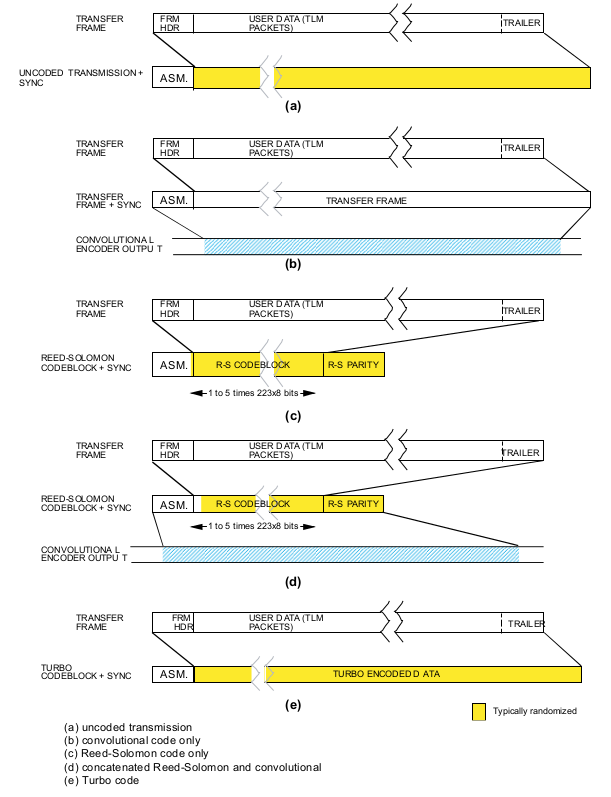
\includegraphics[scale=0.5]{fig/telemetry_link_coding_options}
\caption{Telemetry Link Coding Options}
\label{fig:Telemetry Link Coding Options}
\end{figure}

The \textbf{synchronization} of frames is necessary for the decoding process (if coding is applied) as well as for the pseudo-randomization. An \textbf{attached synch marker} (ASM) is used for this. The ASM is a 32 bit pattern that is fairly unique such that it can be recognized by the receiving end. The specific bit pattern represented in hexadecimal notation is 0x1ACFFC1D, transmitted from left to right. The ASM marks the start of the \textbf{channel access data unit} (CADU). A CADU is therefore defined as a ASM plus the coded or uncoded transfer frame. 

The transfer frame part of the CADU may optionally be exposed to \textbf{pseudo-randomization}. This is done to make the signal have sufficient bit transitions (i.e. avoid having long runs of zeros or ones), which is needed for the receiver to work properly. The pseudo-randomization process is fairly simple: the transfer frame is bitwise exposed to an XOR operation with a pseudo-random sequence, which is generated from the following polynomial: $h(x) = x^{8} + x^{7} +x^{5} + x^{3} + 1$. The sequence generator is initialized with all-ones at the start of each transfer frame.

There is no prescription on how to arrange the CADUs that are sent over the physical channel. Common practice is to send a continuous stream of CADUs back-to-back, and fill them with idle data if no data is available for insertion. A continuous stream of CADUs is essential for the ground receiving end if they only contain idle data, because each CADU also contains valuable information in the frame header and operational control field.

\textbf{Telecommand Synchronization and Channel Coding Sublayer}

\begin{tabular}{l}
\textit{CCSDS-231.0-B "TC Synchronization and Channel Coding" \cite{CCSDS-231.0-B}} \\
\textit{CCSDS-230.1-G "TC Synchronization and Channel Coding--Summary of Concept and Rationale" \cite{CCSDS-230.1-G}}
\end{tabular}

The TC channel coding and synchronization sublayer provides the following four functions for transferring \textbf{telecommand transfer frames} over a space link: error-control coding, synchronization, pseudo-randomization, and repeated transmissions. 

For the \textbf{error-control coding} a modified Bose-Chaudhuri-Hocquenghem (BCH) code is used to reduce the effects of noise in the physical layer and establish a reliable data channel. The BCH codeblock is a fixed-length data entity as shown in Figure \ref{fig:BCH Codeblock Format}. Note that the filler bit is appended to achieve an integer number of bytes per codeblock. It is always set to zero. 

\begin{figure}[h]
\centering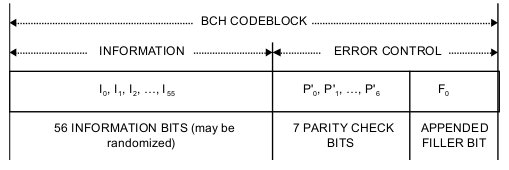
\includegraphics[scale=0.7]{fig/bch_codeblock_format}
\caption{BCH Codeblock Format}
\label{fig:BCH Codeblock Format}
\end{figure}

The parity check bits for each codeblock are generated from a polynomial $g(x) = x^{7} + x^{6} +x^{2} + 1$. It is initialized with all-zeros for each codeblock. Using the parity bits, the receiving end can decode in either error-detecting mode (triple error detection), or in an error-correcting mode (single error correction). 

To achieve \textbf{synchronization} the \textbf{communications link transmission unit} (CLTU) data structure is used. The CLTU is a data structure which carries data as continuous series of encoded BCH codeblocks. The data contained in the BCH codeblocks consist of one or more TC transfer frames from the sublayer above (possibly with fill data). The format of a CLTU is shown in Figure \ref{fig:CLTU Format}. 

\begin{figure}[h]
\centering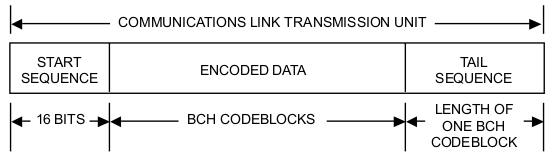
\includegraphics[scale=0.6]{fig/cltu_format}
\caption{CLTU Format}
\label{fig:CLTU Format}
\end{figure}

The start sequence of the CLTU delimits the start of the encoded data within the CLTU. The value of the start sequence in hexadecimal notation is 0xEB90. The encoded data consists of a set of BCH codeblocks, which may have been randomized or not. The tail sequence is a data structure which is constructed specifically to be a noncorrectable sequence which delimits the end of a CLTU by stopping the decoding process. The tail sequence consists of seven bytes of value 0xC5 and one byte with value 0x79. Alternatively the idle sequence consisting of eight bytes of value 0x55 is usable as well.

In order to maintain bit synchronization at the receiving end, the data stream must be sufficiently random. The transfer frame part of the CLTU may therefore optionally be exposed to \textbf{pseudo-randomization}. The pseudo-randomization process is fairly simple: the transfer frame is bitwise exposed to an XOR operation with a pseudo-random sequence, which is generated from the following polynomial: $h(x) = x^{8} + x^{6} +x^{4} + x^{3} + x^{2} + x + 1$. The sequence generator is initialized with all-ones at the start of each transfer frame.

In particular for long-distance links, it is common to send each CLTU with several \textbf{repetitions} in order to increase the likelihood of reception at the receiving end.

The procedure for sending CLTUs over the physical channel is named \textbf{physical layer operation procedure} PLOP. There are two options available, with PLOP-2 being the preferred one. It is defined as follows in terms of \textbf{carrier modulation modes} (CMM):

\begin{enumerate}
\item Begin of command session
\item (CMM-1) Unmodulated carrier only
\item (CMM-2) Carrier modulated with acquisition sequence
\item (CMM-3) Carrier modulated with one CLTU
\item (CMM-4) Carrier modulated with idle sequence 
\item Repeat from step 4 for each CLTU
\item (CMM-1) Unmodulated carrier only
\item End of command session
\end{enumerate}

The acquisition sequence and the idle sequence is a pattern of alternating ones and zeros, starting with either a one or a zero. The acquisition sequence shall be at least 128 bits (16 bytes) long and the idle sequence shall be at least 8 bits long.

\textbf{Telemetry Space Data Link Protocol Sublayer}

\begin{tabular}{l}
\textit{CCSDS-132.0-B "TM Space Data Link Protocol" \cite{CCSDS-132.0-B}} 
\end{tabular}

The telemetry space data link protocol has the features that it is: unidirectional (data flow is one way), unconfirmed service (sending end does not receive confirmation), incomplete service (completeness is not guaranteed), sequence-preserving (the sequence of service data units is preserved, although there may be gaps and duplications).

The telemetry transfer frame is composed of the mandatory and optional fields as shown in Figure \ref{fig:TM Transfer Frame Format}. Although the transfer frame data field is shown with undefined length, the length must be chosen and kept fixed over the mission phase for any channel. Figure \ref{fig:TM Transfer Frame Primary Header Format} shows the format of the primary header.

\begin{figure}[h]
\centering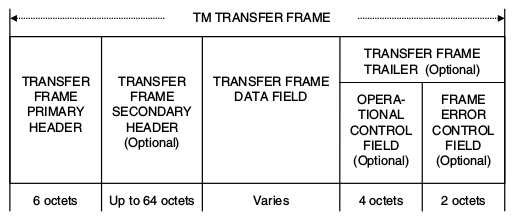
\includegraphics[scale=0.6]{fig/tm_transfer_frame_format}
\caption{TM Transfer Frame Format}
\label{fig:TM Transfer Frame Format}
\end{figure}

\begin{figure}[h]
\centering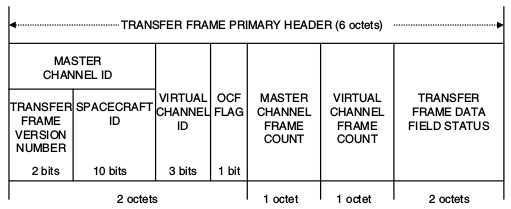
\includegraphics[scale=0.6]{fig/tm_transfer_frame_primary_header_format}
\caption{TM Transfer Frame Primary Header Format}
\label{fig:TM Transfer Frame Primary Header Format}
\end{figure}

The fixed-length TMTF is used to transport variable-length space packets (see Section \ref{sec:Network Layer}) as its service data unit. A TMTF may contain one, several, or zero space packets (in the later case it only contains idle data). Packets are concatenated and inserted into the TMTF until its length is exceeded. Any packet that exceeds the size of the TMTF data field will be split, and starts a new TMTF data field on the same virtual channel with its remainder. For the case where no Packets are available for inserting, idle data is written into the TMTF data field.

The TMTF primary header contains essential information about its source (spacecraft ID) and its channel properties. The data status field provides information about if and where a new packet starts in the data field.

The purpose of the operational control field (OCF) is to provide a mechanism for the retransmission control, namely the communications link control word, as defined in the following.

\textbf{Telecommand Space Data Link Protocol Sublayer}

\begin{tabular}{l}
\textit{CCSDS-232.0-B "TC Space Data Link Protocol" \cite{CCSDS-232.0-B}} \\
\textit{CCSDS-232.1-B "Communications Operation Procedure-1" \cite{CCSDS-232.1-B}}
\end{tabular}

The telecommand space data link protocol has the features that it is: unidirectional (data flow is one way), asynchronous service (data transfer is requested at any time), sequence preserving service (the sequence of service data units is preserved, except for expedited Type-B service).

The telecommand transfer frame is composed of the mandatory and optional fields as shown in Figure \ref{fig:TC Transfer Frame Format}. The transfer frame data field is of variable length. Figure \ref{fig:TC Transfer Frame Primary Header Format} shows the format of the primary header.

\begin{figure}[h]
\centering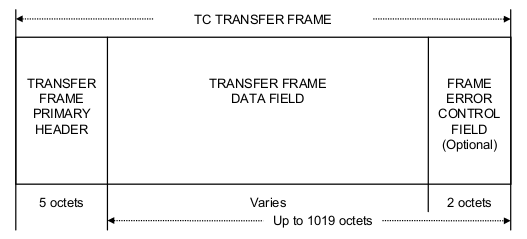
\includegraphics[scale=0.6]{fig/tc_transfer_frame_format}
\caption{TC Transfer Frame Format}
\label{fig:TC Transfer Frame Format}
\end{figure}

\begin{figure}[h]
\centering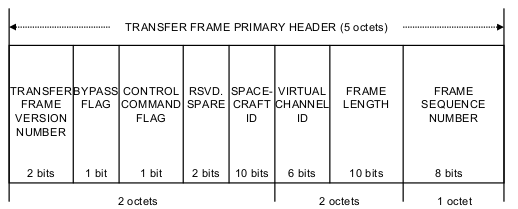
\includegraphics[scale=0.6]{fig/tc_transfer_frame_primary_header_format}
\caption{TC Transfer Frame Primary Header Format}
\label{fig:TC Transfer Frame Primary Header Format}
\end{figure}

The variable-length TCTF is used to transport variable-length space packets (see Section \ref{sec:Network Layer}) as its service data unit. A TCTF may contain one or several space packets. To improve system throughput efficiency, relatively small TCTFs are desirable. Therefore, large space packets are broken into smaller pieces via segmentation and sent in several consecutive TCTFs. On the other hand, very small space packets may be grouped together via blocking and transferred in a single TCTF.

The TCTF primary header contains essential information about its destination (spacecraft ID) and its channel properties. It contains a bypass and control command flag that are used to indicate how sequence control is applied to the frame and what data is contained in the data field:

\begin{itemize}
\item Type-AD: The data field carries space packets, subject to sequence control.
\item Type-BD: The data field carries space packets, bypassing sequence control.
\item Type-BC: The data field carries control commands, bypassing sequence control.
\end{itemize}
 
The transfer frame data field therefore may carry space packet data or control commands. For the case of transferring space packets, a \textbf{segment header} is inserted as the first byte of the data field, with the format defined in Figure \ref{fig:Segment Header Format}. Following the segment header are: a complete packet, multiple packets, or a portion of a packet (Figure \ref{fig:Blocking and Segmentation}). The sequence flags in the segment header are used to distinguish between these cases. Also, the segment header introduced yet another mechanism for further channel multiplexing. Namely it allows the definition of several \textbf{multiplexer access points} (MAP) to be used on a particular virtual channel.

\begin{figure}[h]
\centering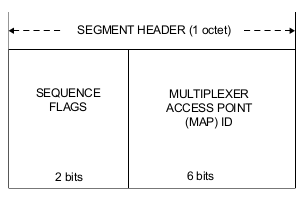
\includegraphics[scale=0.6]{fig/segment_header_format}
\caption{Segment Header Format}
\label{fig:Segment Header Format}
\end{figure}

\begin{figure}[h]
\centering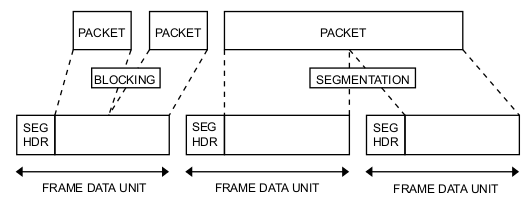
\includegraphics[scale=0.6]{fig/blocking_and_segmentation}
\caption{Blocking and Segmentation}
\label{fig:Blocking and Segmentation}
\end{figure}

For the case where the data field carries \textbf{control commands}, it may contain either  an unlock command, or a command for setting the receiver frame sequence number. These two commands are essential for controlling the sequence control mechanism of the uplink, which is realized through a procedure called communications operation procedure.

The \textbf{communications operation procedure} (COP) is a closed-loop procedure executed by the sending and receiving ends of the telecommand space data link protocol. COP utilizes an automatic request for retransmission (ARQ) procedure to retransmit transfer frames that were rejected by the receiving end. It ensures that Type-AD frames are only accepted at the receiving end in strict sequential order, without omission or duplication. 

COP-1 consists of a pair of synchronized procedures for each virtual channel: a \textbf{frame operation procedure} (FOP-1) at the sending end and a \textbf{frame acceptance and reporting mechanism} (FARM-1) at the receiving end. FOP-1 transmits telecommand transfer frames to the FARM-1 of the same virtual channel. The FARM-1 returns reports of the status of transfer frame acceptance to the FOP-1 using the \textbf{communications link control word} (CLCW), which is placed in the operational control field of a telemetry transfer frame. The format of a CLCW is shown in Figure \ref{fig:Communications Link Control Word Format}.

\begin{figure}[h]
\centering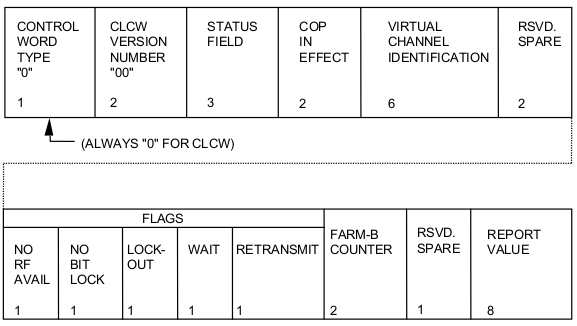
\includegraphics[scale=0.6]{fig/communications_link_control_word_format}
\caption{Communications Link Control Word Format}
\label{fig:Communications Link Control Word Format}
\end{figure}

The \textbf{sequence-controlled service} (also called AD service) is realized through the use of synchronized counters (see Figure \ref{fig: COP-1 Variables, Frame, and Report Values}). For each transmitted and received Type-AD telecommand transfer frame the counter increases on the sending and on the receiving end, respectively. Any loss of transfer frame would result in a mismatch of these counters and will immediately cause the rejection of further incoming telecommand frames.

\begin{figure}[h]
\centering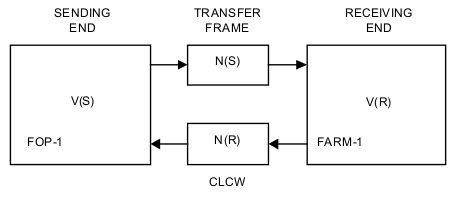
\includegraphics[scale=0.6]{fig/cop-1_variables_frame_and_report_values}
\caption{COP-1 Variables, Frame, and Report Values}
\label{fig: COP-1 Variables, Frame, and Report Values}
\end{figure}

The Type-BC transfer frames are used to carry control commands to configure COP-1, namely to handle locked out situations and to synchronize the counters.

Finally, the expedited service (BD service) is used only in exceptional circumstances, typically during spacecraft recovery. Here the frames are not subjected to sequence control and hence there is no guarantee that all are delivered.

\subsubsection{Network Layer}
\label{sec:Network Layer}

\begin{tabular}{l}
\textit{CCSDS-133.0-B "Space Packet Protocol" \cite{CCSDS-133.0-B}} 
\end{tabular}

The protocol data units used by the network layer are called \textbf{space packets}. Aside from a header that identifies the packet, the internal data content is completely under control of the user application.

The space packets protocol has the features that it is: pre-configured (user data can be sent only through pre-defined logical data path), unidirectional (data flow per defined path is one way), asynchronous (data transfer takes place at any time), unconfirmed service (sending end does not receive confirmation), incomplete service (completeness is not guaranteed), non-sequence-preserving (the sequence of service data units may not be preserved).

The space packet is composed of the fields as shown in Figure \ref{fig:Space Packet Format}. The packet data field is of variable length. Figure \ref{fig:Space Packet Primary Header Format} shows the format of the primary header. The optional packet secondary header may be used to transport time and/or other essential ancillary data in the same location within each and every space packet.

\begin{figure}[h]
\centering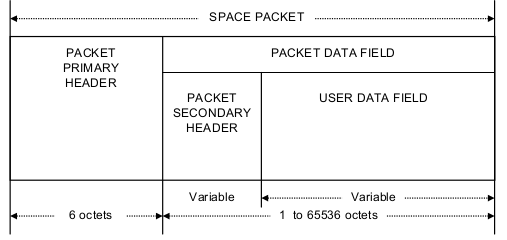
\includegraphics[scale=0.6]{fig/space_packet_format}
\caption{Space Packet Format}
\label{fig:Space Packet Format}
\end{figure}

\begin{figure}[h]
\centering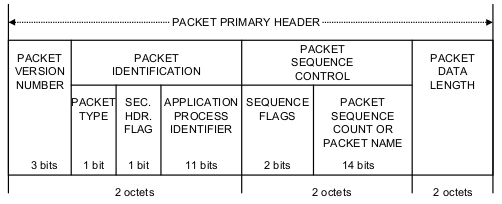
\includegraphics[scale=0.6]{fig/space_packet_primary_header_format}
\caption{Space Packet Primary Header Format}
\label{fig:Space Packet Primary Header Format}
\end{figure}

The \textbf{application process identifier} (APID) is a unique identifier for the sending or receiving application process. The APID is used to identify the \textbf{logical data path} of that particular packet, in order to allow the underlying subnetwork services to route the packet to its destination. 

\subsubsection{Space Link Protocol Stack}

The protocol stack for transport of telecommands and telemetry are shown in Figure \ref{fig:Telecommand Protocol Stack} and Figure \ref{fig:Telemetry Protocol Stack}.

\begin{figure}[h]
\centering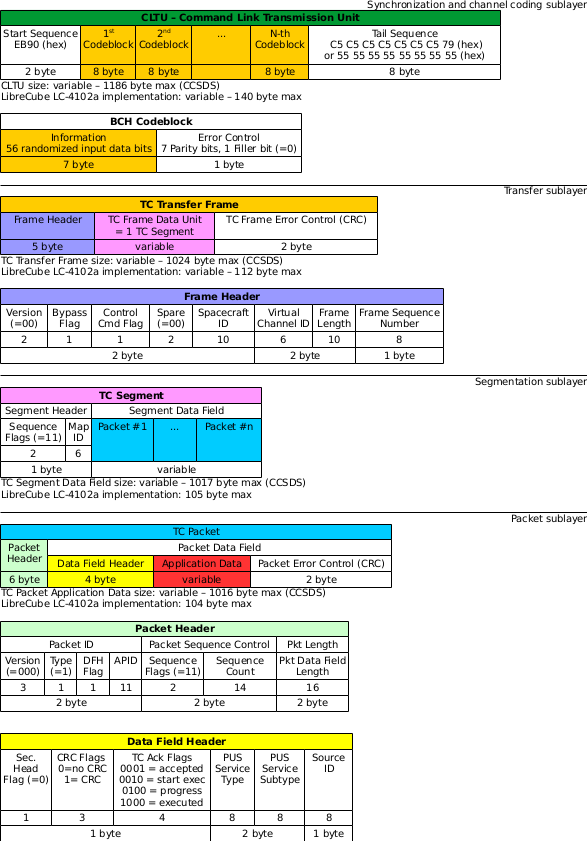
\includegraphics[scale=0.4]{fig/telecommand_protocol_stack}
\caption{Telecommand Protocol Stack}
\label{fig:Telecommand Protocol Stack}
\end{figure}

\begin{figure}[h]
\centering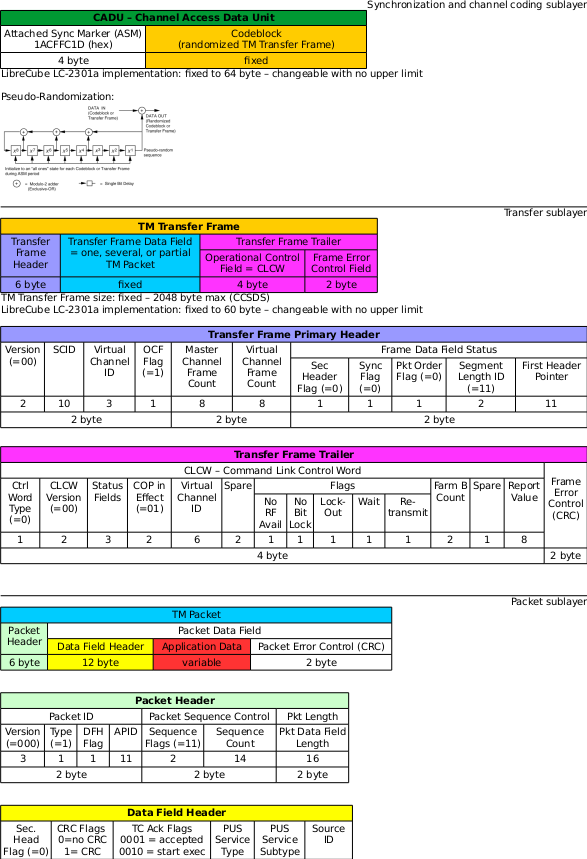
\includegraphics[scale=0.4]{fig/telemetry_protocol_stack}
\caption{Telemetry Protocol Stack}
\label{fig:Telemetry Protocol Stack}
\end{figure}

\clearpage
\subsection{Onboard Interface Services}

\begin{tabular}{l}
\textit{CCSDS-850.0-G "Spacecraft Onboard Interface Services" \cite{CCSDS-850.0-G}} 
\end{tabular}

The spacecraft onboard interface services (SOIS) standardizes the services to be supported by underlying protocols in the onboard software (OBSW) on application support layer and subnetwork layer. Figure \ref{fig:Spacecraft Onboard Interface Services Reference Model} shows a layered view of the recommended services and their associated access points. User, i.e. mission specific applications make use of the \textbf{application support layer} services (and possibly any lower level service). The \textbf{transfer layer} provides transport and network layer services based on existing (or dedicated) protocols (such as space packet for the network protocol). In many cases the transport layer will not be required, unless routing across multiple data links is needed. The \textbf{subnetwork layer} provides access to the data link medium and provides a set of services to be mapped over the subnetwork defined by that medium.

\begin{figure}[h]
\centering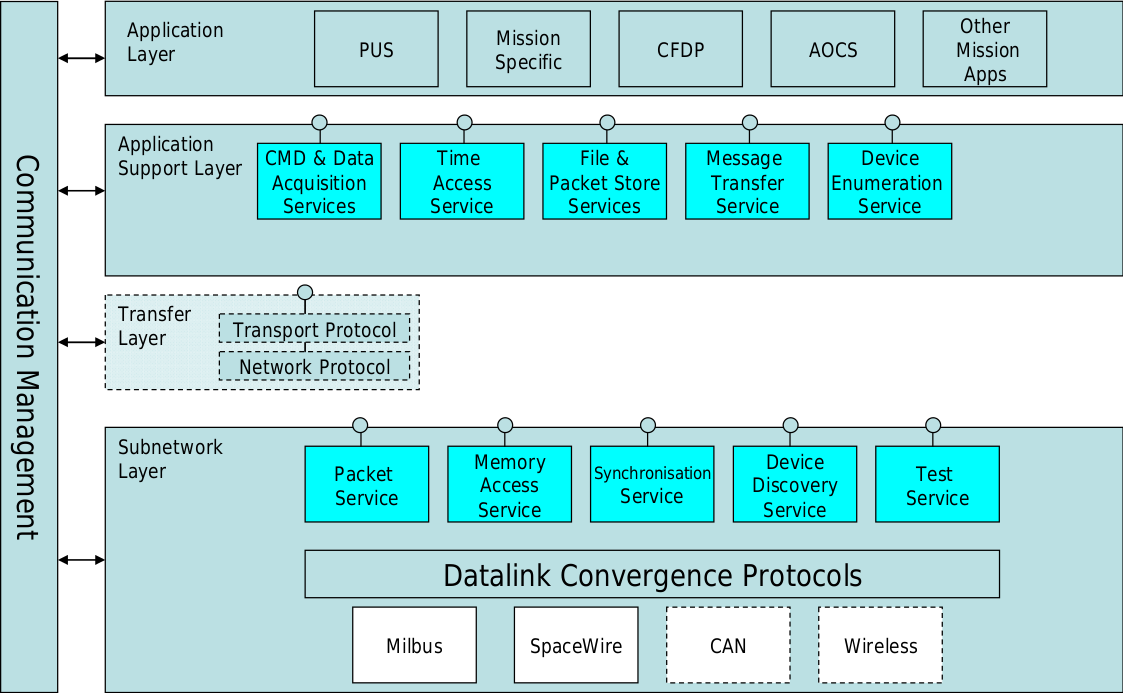
\includegraphics[scale=0.4]{fig/spacecraft_onboard_interface_services_reference_model}
\caption{Spacecraft Onboard Interface Services Reference Model}
\label{fig:Spacecraft Onboard Interface Services Reference Model}
\end{figure}


\subsubsection{Subnetwork Layer - Packet Service}

\begin{tabular}{l}
\textit{CCSDS-851.0-M "Spacecraft Onboard Interface Services--Subnetwork Packet Service" \cite{CCSDS-851.0-M}} 
\end{tabular}

The \textbf{packet service} transfers variable length, delimited octet strings from one endpoint on a data link to another endpoint within the same subnetwork. It defines four classes of quality of service (QoS) for the transfer and provides the following three primitives: packet send request, packet receive indication, and packet failure indication (depending on the QoS).

\subsubsection{Subnetwork Layer - Memory Access Service}

\begin{tabular}{l}
\textit{CCSDS-852.0-M "Spacecraft Onboard Interface Services--Subnetwork Memory Access Service" \cite{CCSDS-852.0-M}} 
\end{tabular}

The \textbf{memory access service} provides means for a user entity to retrieve or change data located in memory hosted by a node on a subnetwork. The QoS comprises acknowledgement, authorisation, priority, and other aspects. The service provides the following primitives: read request, read indication, write request, an atomic read/modify/write request (useful for example to set individual bits), and a memory access result indication (as a response to the write and atomic read/modify/write).

\subsubsection{Subnetwork Layer - Subnetwork Synchronisation Service}

\begin{tabular}{l}
\textit{CCSDS-853.0-M "Spacecraft Onboard Interface Services--Subnetwork Synchronisation Service" \cite{CCSDS-853.0-M}} 
\end{tabular}

The \textbf{synchronisation service} provides a means for a user entity to maintain knowledge of time which is common to all data systems on the subnetwork. It is a best-effort service which provides the following primitives: time request, time indication, and optionally also: event request, event indication.

\subsubsection{Subnetwork Layer - Subnetwork Device Discovery Service}

\begin{tabular}{l}
\textit{CCSDS-854.0-M "Spacecraft Onboard Interface Services--Subnetwork Device Discovery Service" \cite{CCSDS-854.0-M}} 
\end{tabular}

The \textbf{device discovery service} provides a means for a user entity to receive notification of the presence of other nodes on the subnetwork. It is a best-effort service which provides the following primitives: device discovery request, device discovery indication, and device discovery loss indication.

\subsubsection{Subnetwork Layer - Subnetwork Test Service}

\begin{tabular}{l}
\textit{CCSDS-855.0-M "Spacecraft Onboard Interface Services--Subnetwork Test Service" \cite{CCSDS-855.0-M}} 
\end{tabular}

The \textbf{test service} provides a means for a user entity to test functionality and connectivity of the subnetwork. It is a best-effort service, which provides the following primitives: test request and test indication.

\subsubsection{Application Support Layer - Command and Data Acquisition Services}

The \textbf{command and data acquisition services} provide the ability for onboard applications to command and acquire data from onboard devices across subnetworks, whilst being isolated from the protocols associated with the particular subnetworks. Applications can interface to the functionality directly provided by a physical device or with a higher level abstraction of the physical device, known as a virtual device. The individual services that comprise the command and data acquisition services are described in the following.

\begin{tabular}{l}
\textit{CCSDS-871.0-M "Spacecraft Onboard Interface Services--Device Access Service" \cite{CCSDS-871.0-M}} 
\end{tabular}

The \textbf{device access service} (DAS) provides a standard interface between onboard software applications and flight hardware such as sensors and actuators. To acquire a value (i.e. data) from a device, an application invokes the "acquire from device request" primitive and obtains the result in form of an "acquire from device indication" primitive. To command (i.e. send a value to) a device, an application invokes the "command device request" primitive and obtains the result in form of an "command device indication" primitive, which indicates whether or not the command was sent successfully and, if available, more result metadata. The DAS uses either the packet service or the memory access service form the subnetwork layer to implement its functionality. An example is shown in Figure \ref{fig:Example Device Access Service}.

\begin{figure}[h]
\centering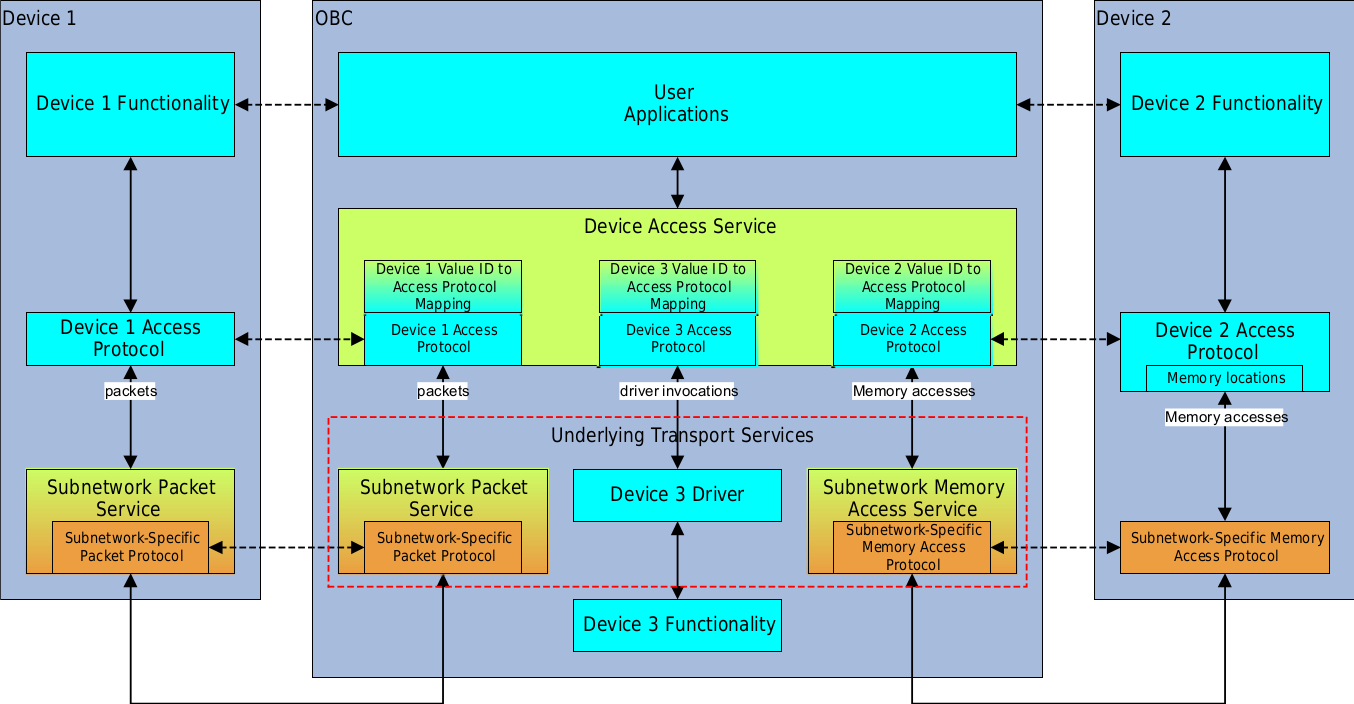
\includegraphics[scale=0.3]{fig/example_device_access_service}
\caption{Example Device Access Service}
\label{fig:Example Device Access Service}
\end{figure}

\begin{tabular}{l}
\textit{CCSDS-871.2-M "Spacecraft Onboard Interface Services--Device Virtualization Service" \cite{CCSDS-871.2-M}} 
\end{tabular}

The \textbf{device virtualization service} (DVS) provides applications with functional interfaces to devices, abstracted from the protocols used for accessing the devices and the data encodings used in those protocols. This is a further abstraction on top of the device access service that provides applications with raw interfaces to devices, only abstracted from the subnetwork protocols used for exchanging data with the devices. Similar to the DAS, the DVS provides service primitives for commanding and data acquisitions. In contrast however, it uses logical identifiers for the device and value identifiers, which are then mapped to the physical ones via a managed \textbf{device and value identifier resolution table}.

An example would be to command ON a virtual image of a GPS unit via the DVS, which then invokes a number of DAS functions to implement this functionality. the required mapping of identifiers for each service layer is shown in Figure \ref{fig:Mapping of Identifiers}.

\begin{figure}[h]
\centering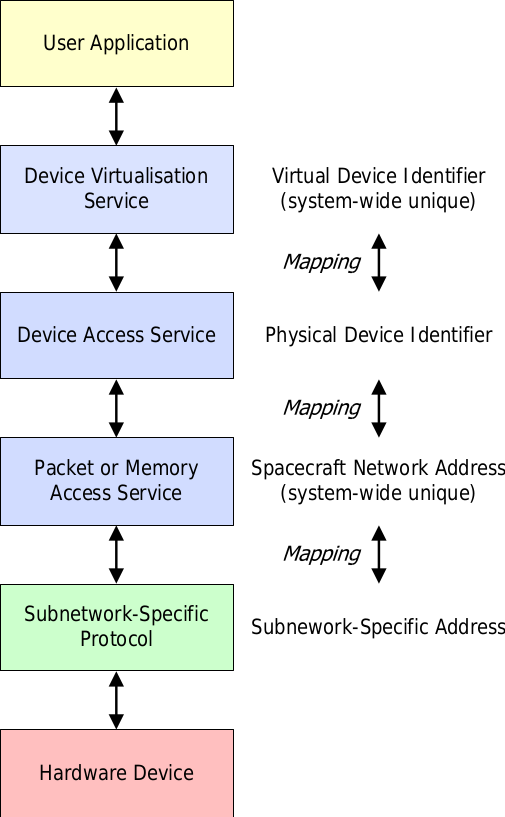
\includegraphics[scale=0.3]{fig/mapping_of_identifiers}
\caption{Mapping of Identifiers}
\label{fig:Mapping of Identifiers}
\end{figure}

\begin{tabular}{l}
\textit{CCSDS-871.1-M "Spacecraft Onboard Interface Services--Device Data Pooling Service" \cite{CCSDS-871.1-M}} 
\end{tabular}

The \textbf{device data pooling service} (DDPS) enables onboard software to access pooled data acquired from simple onboard hardware devices such as sensors and actuators, without explicitly requesting an acquisition from the real device. The layout of a data pool is shown in Figure \ref{fig:Layout of Data Pool}. At each sample acquisition, the various pre-defined values are sampled and stored together with a time stamp. A (normally short) history of those samples is maintained.

\begin{figure}[h]
\centering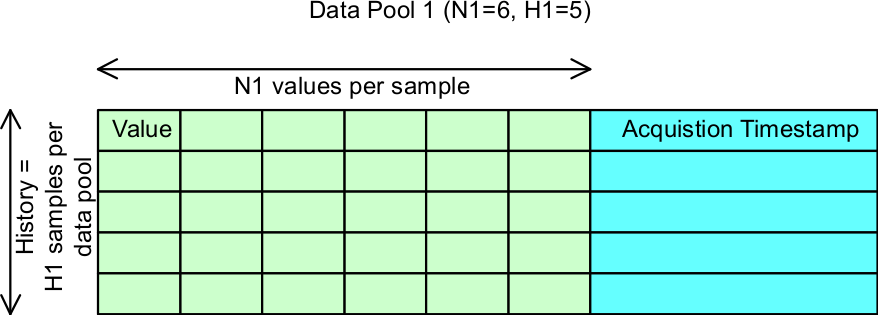
\includegraphics[scale=0.3]{fig/layout_of_data_pool}
\caption{Layout of Data Pool}
\label{fig:Layout of Data Pool}
\end{figure}

The sample acquisition period can be conveniently synchronized using the subnetwork synchronization service. This is shown in Figure \ref{fig:Example of Data Pooling Service}.

\begin{figure}[h]
\centering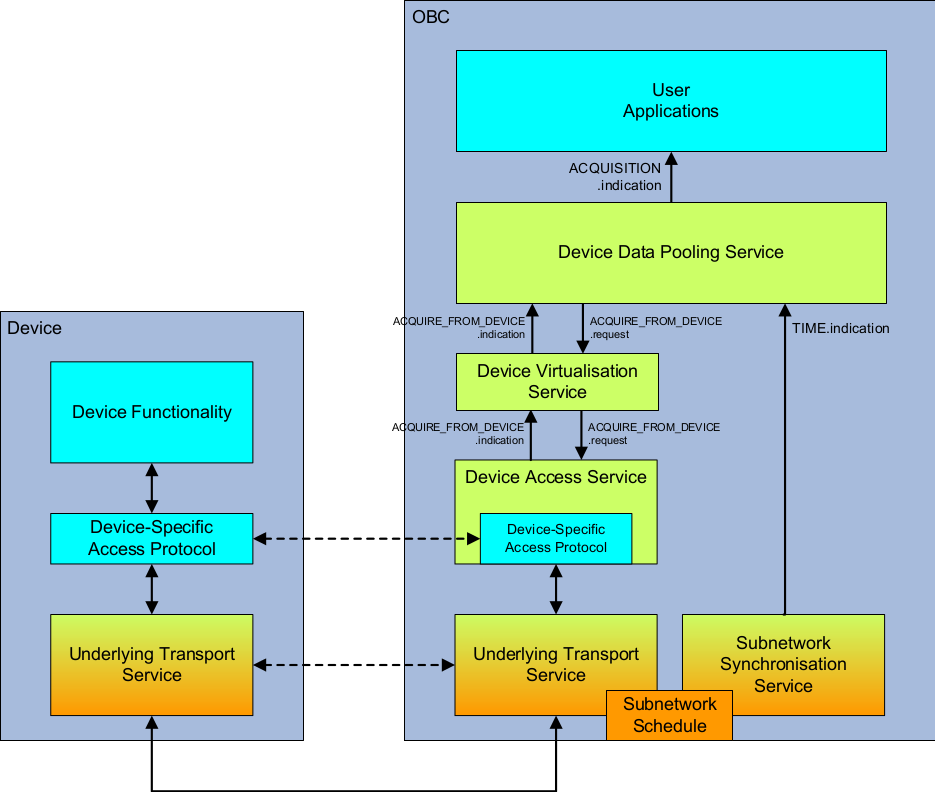
\includegraphics[scale=0.3]{fig/example_of_data_pooling_service}
\caption{Example of Data Pooling Service}
\label{fig:Example of Data Pooling Service}
\end{figure}

The DDPS provides service primitives for creating, deleting, starting, and stopping such data pools, and for reading them.

\begin{tabular}{l}
\textit{CCSDS-871.3-M "Spacecraft Onboard Interface Services--Device Enumeration Service" \cite{}} 
\end{tabular}

The \textbf{device enumeration service} (DES) provides management and user notification of addition of devices to or removal of devices from a spacecraft. The main goal of DES is to assist onboard reconfiguration functions, such as mode management or fault detection, isolation, and recovery regarding the notification of changes in the spacecraft configuration, and the execution of operations needed to adjust the onboard software to the new configuration. An example is given in Figure \ref{fig:Device Enumeration Service and Redundancy}.

\begin{figure}[h]
\centering\includegraphics[scale=0.3]{fig/device_enumeration_service_and_redundancy}
\caption{Device Enumeration Service and Redundancy}
\label{fig:Device Enumeration Service and Redundancy}
\end{figure}

The DES provides service primitives for adding, removing, querying/enumerating of devices, and indications of devices found or lost. Its relationship with other SOIS services is shown in Figure \ref{fig:Relationship between Device Enumeration Service and other Services}.

\begin{figure}[h]
\centering\includegraphics[scale=0.3]{fig/relationship_between_device_enumeration_service_and_other_services}
\caption{Relationship between Device Enumeration Service and other Services}
\label{fig:Relationship between Device Enumeration Service and other Services}
\end{figure}

\subsubsection{Application Support Layer - Time Access Services}

\begin{tabular}{l}
\textit{CCSDS-872.0-M "Spacecraft Onboard Interface Services--Time Access Service" \cite{}} 
\end{tabular}

The \textbf{time access service} provides a user entity with a consistent interface to a local time source that is correlated to some centrally maintained master onboard time source. The local time sources are typically free-running hardware counters accumulating seconds and sub-seconds of elapsed time. The master time source usually has the most accurate precision and broadcasts its time information to the other entities on the subnetwork, via the synchronisation service (see Figure \ref{fig:Typical Onboard Time System Architecture}). 

\begin{figure}[h]
\centering\includegraphics[scale=0.3]{fig/typical_onboard_time_system_architecture}
\caption{Typical Onboard Time System Architecture}
\label{fig:Typical Onboard Time System Architecture}
\end{figure}

Applications should use this service to obtain the time from the local time source rather than, for example, reading directly from the local elapsed time counter hardware registers. The service primitives provide are: time request and time indication for the so-called wall clock capability, and optionally, various primitives for implementing the alarm clock and metronome capability. 

\subsubsection{Application Support Layer - File and Packet Store Services}

\begin{tabular}{l}
\textit{CCSDS-873.0-M "Spacecraft Onboard Interface Services--Time Access Service" \cite{}} 
\end{tabular}

The \textbf{file and packet store services} (FPSS) comprise the following services: file access service (FAS), file management service (FMS), packet store access service (PSAS), and packet store management service (PSMS). These services are used to access and manage files and packets residing in file and packet stores. A \textbf{file store} is considered to be a file system (flat or hierarchical) and the associated storage medium. A \textbf{packet store} does not use a file system, but instead is organized either as an bounded or circular first-in first-out (FIFO) store, or a random-access store (the later being much more complex to manage). A large number of primitives are defined for each service to provide the functionality of accessing and managing the contents of the stores. An example deployment is shown in Figure \ref{fig:Example Deployment of Packet Store} where packets are stored in the onboard solid state mass memory (SSMM).

\begin{figure}[h]
\centering\includegraphics[scale=0.3]{fig/example_deployment_of_packet_store}
\caption{Example Deployment of Packet Store}
\label{fig:Example Deployment of Packet Store}
\end{figure}

\subsubsection{Application Support Layer - Message Transfer Service}

\begin{tabular}{l}
\textit{CCSDS-875.0-M "Spacecraft Onboard Interface Services--Message Transfer Service" \cite{}} 
\end{tabular}

The \textbf{message transfer service} (MTS) provides applications with a standard service for mediating the transfer of discrete data, i.e. messages, between onboard software users in a (potentially) distributed onboard system.

Four different models of message transfer exist:
\begin{itemize}
\item Send/receive: Messages may simple be sent to designated modules.
\item Synchronous query: Messages may be sent asynchronously but allowing synchronization with the message reply.
\item Publish/subscribe: Messages may be published to a time-varying number of self-selected subscribers.
\item Announcement: Messages may be sent to a set of modules selected by the message source.
\end{itemize}

The SOIS MTS is essentially a subset of the asynchronous message service (AMS). It provides a large number of service primitives with tailoring in respect to the MTS service definition.

\subsubsection{Electronic Data Sheets}

\begin{tabular}{l}
\textit{CCSDS-876.0-R "Spacecraft Onboard Interface Services--XML Specification for Electronic Data Sheets for Onboard Devices" \cite{}} \\
\textit{CCSDS-876.1-R "Spacecraft Onboard Interface Services--Common Dictionary of Terms for Onboard Devices and Software Components" \cite{}}
\end{tabular}

The \textbf{SOIS electronic datasheets} (SEDS) are intended to be a machine-understandable mechanism for describing devices which may be accessed using the SOIS command and data acquisition services. In this way it potentially shall replace the traditional user manuals, interface control documents, and datasheets which accompany a device and are necessary to determine the operation of the device and how to communicate with it.

The SEDS describes the format of information in a data interface for an onboard device accessed using the command and data acquisition service of the application support layer and the packet and memory access service of the subnetwork layer.

The SEDS are in XML format and specified by an XSD schema that allows for checking correct syntax. In addition, there is also a dictionary of terms (DoT) defined, which provides for semantic correctness checking. 

\subsection{Onboard Software Applications}
\label{sec:Onboard Software Applications}

\subsubsection{File Exchange Applications}

\begin{tabular}{l}
\textit{CCSDS-727.0-B "CCSDS File Delivery Protocol (CFDP)" \cite{CCSDS-727.0-B}} \\
\textit{CCSDS-720.1-G "CCSDS File Delivery Protocol (CFDP) Part 1: Introduction and Overview" \cite{CCSDS-720.1-G}} \\
\textit{CCSDS-720.2-G "CCSDS File Delivery Protocol (CFDP) Part 2: Implementers Guide" \cite{CCSDS-720.2-G}} \\
\end{tabular}

This standard defines a protocol suitable for the transmission of files to and from spacecraft data storage and capable of operating in a wide variety of mission configurations. In addition to the purely file delivery related functions, the protocol includes file management services to allow control over the storage medium. Although the protocol can operate over a wide range of subnetwork services, this standard assumes the use of existing CCSDS packet services. 

The CFDP enables the moving of a file from one filestore to another, where the two filestores are in general resident in separate data systems and often with an intervening space link. In its simplest form, the protocol provides a Core file delivery capability operating across a single link. For more complex mission scenarios, the protocol offers extended operation providing store-and-forward functionality across an arbitrary network, containing multiple links with disparate availability, as well as subnetworks with heterogeneous protocols (Figure \ref{fig:CCSDS File Delivery Protocol}).

\begin{figure}[h]
\centering\includegraphics[scale=0.4]{fig/cfdp}
\caption{CCSDS File Delivery Protocol}
\label{fig:CCSDS File Delivery Protocol}
\end{figure}

\subsubsection{Packet Utilization Services}

\begin{tabular}{l}
\textit{ECSS-E-ST-70-41 "Telemetry and telecommand packet utilization" \cite{ECSS-E-ST-70-41}} \\
\end{tabular}

The packet utilization standard (PUS) addresses the utilization of telecommand packets and telemetry packets for the purposes of remote monitoring and control of spacecraft subsystems and payloads. It is defining the application level interface between ground and space, in order to satisfy the requirements of electrical integration and testing and flight operations.

The services defined by PUS cover a wide spectrum of operational scenarios and, for a given mission, only a subset of these services is likely to be appropriate. The PUS should be viewed as a "Menu" from which the applicable services and service levels are selected for a given mission. The specification of PUS services is adapted to the expectation that different missions require different levels of complexity and capability from a given service. 

The standardized PUS services fulfill the following criteria:
\begin{itemize}
\item Commonality: each standard service corresponds to a group of capabilities applicable to many missions.
\item Coherence: the capabilities provided by each standard service are closely related and their scope is unambiguously specified. Each standard service covers all the activities for managing interrelated state information and all activities that use that state information.
\item Self-containment: each standard service has minimum and well-defined interactions with other services or on-board functions.
\item Implementation independence: the standard services neither assume nor exclude a particular spacecraft architecture (hardware or software).
\end{itemize}

The standard service types are shown in Figure \ref{fig:PUS Services}. They include:

\begin{itemize}
\item Service types that provide basic functions such as collecting parameter statistics.
\item Service types that hold requests and release them to another service as appropriate. The time-based scheduling, the position-based scheduling and the event-action service types are examples of service types that hold and release requests following the occurrences of specified events.
\item Service types that provide standardized interfaces, for example to onboard devices, to an onboard control procedure engine or to an onboard file handling system.
\end{itemize}

\begin{figure}[h]
\centering\includegraphics[scale=0.5]{fig/pus_services}
\caption{PUS Services}
\label{fig:PUS Services}
\end{figure}

When applying the PUS standard, a mission instantiates this standard by tailoring it for their needs. That instantiation results in a mission-specific packet utilization definition document that is rendered applicable to all partners involved in that mission. This document contains the mission-specific service type model that includes all PUS standardized service types considered suitable for use by that mission, each one tailored according to the mission needs, and all mission-specific additional service types.

\subsubsection{Onboard Control Procedures}

\begin{tabular}{l}
\textit{ECSS-E-ST-70-01 "Spacecraft on-board control procedures" \cite{ECSS-E-ST-70-01}} \\
\end{tabular}

The onboard control procedure (OBCP) concept is that of a procedure to be executed onboard, which can easily be loaded, executed, and also replaced, onboard the spacecraft without modifying the remainder of the onboard software. 

The benefits of implementing traditional onboard software (OBSW) functions as OBCPs include:
\begin{itemize}
\item the relative ease of development and validation of OBCPs vs. OBSW;
\item the core OBSW can be made more generic and is hence potentially reusable across many missions, if mission-specific functions are implemented as OBCPs; 
\item simplification of the OBSW maintenance task, i.e. changes to OBCPs can be easily and safely performed without changing the core OBSW. 
\end{itemize}

The availability of OBCPs enables operations procedures (both for routine functions and contingency operations) to be executed onboard as an alternative to on the ground (either  under manual control or automated in the mission control system). This can streamline the operations (reduction of bandwidth, potential reduction in operations manpower, reduction in  the loop delay inherent in ground control, simplification of ground procedures) as well as increasing their overall reliability. The use of  OBCPs also enhances the onboard autonomy capabilities and increases the robustness to ground station outages. 



\chapterimage{chapter_head_01} % Chapter heading image
\chapter{Ground Segment}

\section{Overview}

The ground segment comprises those elements of the space mission that are used to control the spacecraft and its payload, and to process the data returned from it. The activities can be divided into two general domains: control and monitoring of the spacecraft platform, and operation and exploitation of the payload.

\section{Ground Station System}

For everything related to the space link (i.e. that radio communications path between ground and space segment), the standards presented in section \ref{sec:Space Link} apply.

\begin{tabular}{l}
\textit{"Ground Equipment Monitoring Service (GEMS)" \cite{GEMS}} \\
\end{tabular}

The GEMS specification defines a standard, platform independent model (PIM) for controlling a wide range of devices used as ground station equipment. The GEMS model does not presume or try to define a specific system level architecture. Instead, it defines generic concepts such as devices, parameters, and directives that are relatively simple to implement and provide system integrators common ways to control heterogeneous suites of space related ground equipment. The central concept of GEMS is the GEMS device. GEMS devices have typed parameters, accept directives with typed arguments, and can optionally save and restore their configuration using persistent storage. Users utilize the GEMS interface within the device to configure and obtain status.

The specification defines a simple ASCII message protocol usable across a variety of transport mechanisms, including networks, serial lines and internal data buses. The message structure is human-readable and easy to process.

\section{Ground Communications System}

\begin{tabular}{l}
\textit{CCSDS-910.0-G "Space Link Extension Services - Executive Summary" \cite{CCSDS-910.0-G}} \\
\textit{CCSDS-910.3-G "Cross Support Concept — Part 1:  Space Link Extension" \cite{CCSDS-910.3-G}} \\
\textit{CCSDS-910.4-B "Cross Support Reference Model—Part 1: Space Link Extension Services" \cite{CCSDS-910.4-B}} \\
\end{tabular}

The space link extension (SLE) services extend the return telemetry (TM) and forward telecommand (TC) space link services (see \ref{sec:Space Link} and \ref{fig:Domain of Space Link and Space Link Extension Services}) in terms of: over (ground) distance, in time, and/or by adding information.

\begin{figure}[h]
\centering\includegraphics[scale=0.5]{fig/domains_of_space_link_and_space_link_extension_services}
\caption{Domain of Space Link and Space Link Extension Services (CCSDS)}
\label{fig:Domain of Space Link and Space Link Extension Services}
\end{figure}

The SLE services include two major elements:

\begin{itemize}
\item data transfer services that move space link data units between ground stations, control centers, and end-user facilities;
\item management services that control the scheduling and provisioning of the transfer services.
\end{itemize}

The SLE services operate in two phases:

\begin{itemize}
\item the definition phase, when most of the management activities take place;
\item the utilization phase, when the data transfer takes place (this can be either in real-time or off-line with respect to the contact time with the spacecraft).
\end{itemize}

The adherence to SLE standards makes it possible to implement cross support among ground station providers and satellite operators. Due to the well defined SLE interfaces and functionality if SLE elements, a large number of different cross support scenarios are feasible. For example, Figure \ref{fig:Multiple Limited Capability Ground Stations} illustrates the case in which multiple minimal ground stations each send all frames received during a pass to a single complex. This complex performs all the remaining return processing and distributes the data to users. Similarly, this complex accepts forward data from users, processes it, and transmits it to the ground stations for transmission to the mission spacecraft.

\begin{figure}[h]
\centering\includegraphics[scale=0.5]{fig/multiple_limited_capability_ground_stations}
\caption{Multiple Limited Capability Ground Stations (CCSDS)}
\label{fig:Multiple Limited Capability Ground Stations}
\end{figure}

\subsection{SLE Service Management}

\begin{tabular}{l}
\textit{CCSDS-910.14-G "Space Communication Cross Support — Service Manag. — Operations Concept" \cite{CCSDS-910.14-G}} \\
\textit{CCSDS-910.11-B "Space Communication Cross Support — Service Manag. — Service Specification" \cite{CCSDS-910.11-B}} \\
\end{tabular}

Although the SLE data transfer services can be implemented with an ad-hoc (user agreed) service management, adhering to the SLE service management standard provides a formal and clear definition of services for negotiation, configuration, and execution of space link services, and thus allows for maximum of automation of this tasks. 

The service management functions are implemented by the utilization management (UM) on the user side and the complex management (CM) on the provider side (see Figure \ref{fig:Service Management Environment}). The following four services are defined:

\begin{itemize}
\item Service package service, which addresses the arrangement of spacecraft space link session times and execution of the SLE transfer services.
\item Configuration profile service, which addresses the establishment of sets of data concerning the space link and ground station configuration.
\item Trajectory prediction service, which addresses the transfer and updating of spacecraft trajectory data.
\item Service agreement service, which addresses the information that needs to be agreed upon before a cross support service can be established.
\end{itemize}

\begin{figure}[h]
\centering\includegraphics[scale=0.3]{fig/service_management_environment}
\caption{Service Management Environment (CCSDS)}
\label{fig:Service Management Environment}
\end{figure}

\subsection{SLE Transfer Services}

The SLE transfer services are a suite of services that are used to transfer specific telecommand and telemetry protocol data units. The transfer services for the forward and return space link are presented in the next sections. There are three modes of delivery for SLE transfer services:

\begin{itemize}
\item complete online, where service data is delivered in the sequence received, with no data omitted (may relay on sufficient buffering capabilities);
\item timely online, where data may be omitted (deleted) if it exceeds a defined maximum delivery delay;
\item offline, where data is transported outside a real-time space link session.
\end{itemize}

\subsubsection{Return SLE Services}

\begin{tabular}{l}
\textit{CCSDS-911.1-B "Space Link Extension — Return All Frames Service Specification" \cite{CCSDS-911.1-B}} \\
\textit{CCSDS-911.2-B "Space Link Extension — Return Channel Frames Service Specification" \cite{CCSDS-911.2-B}} \\
\textit{CCSDS-911.5-B "Space Link Extension — Return Operational Control Fields Service Specification" \cite{CCSDS-911.5-B}} \\
\end{tabular}

The return SLE services (shown in Figure \ref{fig:Return SLE Services}) include: 

\begin{itemize}
\item Return all frames (RAF): provides the telemetry frames from a single space link symbol stream to spacecraft operators and other users who might need all the frames;
\item Return channel frames (RCF): provides master channel (MC) or specific virtual channels (VCs), as specified by each RCF service user;
\item Return frame secondary header (RFSH): provides MC or VC frame secondary headers (FSHs), as specified by each RFSH service user; 
\item Return operational control field (ROCF): provides MC or VC operational control fields (OCFs) channel, as specified by each ROCF service user; 
\item Return space packet (RSP): enables single users to receive packets with selected application process identifiers (APIDs) from one spacecraft VC.
\end{itemize}

\begin{figure}[h]
\centering\includegraphics[scale=0.3]{fig/return_sle_services}
\caption{Return SLE Services (CCSDS)}
\label{fig:Return SLE Services}
\end{figure}

\subsubsection{Forward SLE Services}

\begin{tabular}{l}
\textit{CCSDS-912.1-B "Space Link Extension — Forward CLTU Service Specification" \cite{CCSDS-912.1-B}} \\
\textit{CCSDS-912.3-B "Space Link Extension — Forward Space Packet Service Specification" \cite{CCSDS-912.3-B}} \\
\end{tabular}

The forward SLE services (shown in Figure \ref{fig:Forward SLE Services}) include: 

\begin{itemize}
\item Forward space packet (FSP): enables single users to provide packets for uplink to a spacecraft without needing to co-ordinate with other users of the spacecraft;
\item Forward telecommand virtual channel access (FTCVCA): enables users to provide complete VCs for uplink;
\item Forward telecommand frame (FTCF): enables users to supply TC frames to be transformed to communications link transmission units (CLTUs) ready for uplink;
\item Forward communications link transmission unit (FCLTU): enables users to provide CLTUs for pulink to the spacecraft.
\end{itemize}

\begin{figure}[h]
\centering\includegraphics[scale=0.4]{fig/forward_sle_services}
\caption{Forward SLE Services (CCSDS)}
\label{fig:Forward SLE Services}
\end{figure}

Note that as shown in Figure \ref{fig:Forward SLE Services} the ROCF service is input to the CLTU production and VC and packet production service.

\subsection{Cross Support Transfer Services}

\begin{tabular}{l}
\textit{CCSDS-921.1-R "Cross Support Transfer Service - Specification Framework" \cite{CCSDS-921.1-R}} \\
\end{tabular}

Cross support transfer services (CSTSes) provide for reliable, access-controlled transfer of spaceflight mission related data between ground element entities. A cross support service is characterized by the kind of data it transfers (e.g., telemetry data,  tracking data, service production monitoring data), and therefore different CSTSes need  to respond to specific requirements that may demand specific solutions. On the other hand, all CSTSes defined by CCSDS  apply the same basic communications patterns in order  to simplify specification, implementation, and operation of these services.  

\begin{tabular}{l}
\textit{CCSDS-922.1-R "Cross Support Transfer Service - Monitored Data Service" \cite{CCSDS-922.1-R}} \\
\end{tabular}

This standard defines a service, which allows a spaceflight mission to receive cyclic reports on, and to query the current values of, the parameters that are pertinent to cross support services being provided by a cross support complex. The service also allows a spaceflight mission to receive notifications of the occurrence of events of interest associated with the services that are being provided by the complex.

\begin{tabular}{l}
\textit{CCSDS-922.2-R "Cross Support Transfer Service - Tracking Data Cross support Transfer Service" \cite{CCSDS-922.2-R}} \\
\end{tabular}

This standard defines a service that allows a spaceflight mission to receive periodic measurements of tracking data as soon as they are generated by a cross support complex or anytime thereafter. The service delivers the tracking data formatted in accordance with the CCSDS Tracking Data Message Recommended Standard (TDM).

\subsection{API for Transfer Services}

\begin{tabular}{l}
\textit{CCSDS-914.1-G "SLE — API for Transfer Services — Summary of Concept and Rationale" \cite{CCSDS-914.1-G}} \\
\textit{CCSDS-914.0-M "SLE — API for Transfer Services — Core Specification" \cite{CCSDS-914.0-M}} \\
\textit{CCSDS-914.2-G "SLE — API for Transfer Services — Application Programmer's Guide" \cite{CCSDS-914.2-G}} \\
\end{tabular}

The SLE API provides a high level, communication technology independent interface for exchange of SLE operation invocations and returns between a SLE service user and a SLE service provider. 

The SLE API for transfer services consists of two distinct layers, API proxy and the API service element, shown shown in figure \ref{fig:Layers of the SLE API}.

\begin{figure}[h]
\centering\includegraphics[scale=0.5]{fig/layers_of_the_sle_api}
\caption{Layers of the SLE API (CCSDS)}
\label{fig:Layers of the SLE API}
\end{figure}

The API proxy represents the technology abstraction layer. 

\subsubsection{API for Return SLE Services}

\begin{tabular}{l}
\textit{CCSDS-915.1-M "Space Link Extension — API for Return All Frames Service" \cite{CCSDS-915.1-M}} \\
\textit{CCSDS-915.2-M "Space Link Extension — API for Return Channel Frames Service" \cite{CCSDS-915.2-M}} \\
\textit{CCSDS-915.5-M "Space Link Extension — API for Return Operational Control Fields" \cite{CCSDS-915.5-M}} \\
\end{tabular}

These standards define C++ application program interfaces (APIs) for the specified return SLE services.

\subsubsection{API for Forward SLE Services}

\begin{tabular}{l}
\textit{CCSDS-916.1-M "Space Link Extension — API for the Forward CLTU Service" \cite{CCSDS-916.1-M}} \\
\textit{CCSDS-916.3-M "Space Link Extension — API for the Forward Space Packet Service" \cite{CCSDS-916.3-M}} \\
\end{tabular}

These standards define C++ application program interfaces (APIs) for the specified forward SLE services.

\subsubsection{Internet Protocol for Transfer Services}

\begin{tabular}{l}
\textit{CCSDS-913.1-B "Space Link Extension — Internet Protocol for Transfer Services" \cite{CCSDS-913.1-B}} \\
\end{tabular}

This standard defines a protocol for transfer of SLE protocol data units (PDUs) using the internet protocols TCP (transmission control protocol) and IP (internet protocol), named internet SLE protocol one (ISP1). It is a layered protocol as shown in Figure \ref{fig:ISP1 Architectural Model}, where the:

\begin{itemize}
\item Higher layers: represent the functionality specified in the SLE transfer services;
\item Authentication layer: responsible for generating and analysing the credentials to authorize transfers;
\item Data encoding layer: responsible for encoding of SLE protocol data units received from higher layers and decoding of protocol data units received from the peer application;
\item Transport mapping layer: handles the interface to the TCP protocol.
\end{itemize}

\begin{figure}[h]
\centering\includegraphics[scale=0.4]{fig/isp1_architectural_model}
\caption{ISP1 Architectural Model (CCSDS)}
\label{fig:ISP1 Architectural Model}
\end{figure}

\section{Mission Operations System}

\subsection{Spacecraft Control System}

For everything related to the application layer functionality of the spacecraft control system (that is, the packet utilization standard and the CCSDS file delivery protocol), the standards presented in section \ref{sec:Onboard Software Applications} apply accordingly.

\subsubsection{Mission Information Base}

\begin{tabular}{l}
\textit{CCSDS-660.0-B "XML Telemetric and Command Exchange (XTCE)" \cite{CCSDS-660.0-B}} \\
\textit{CCSDS-660.0-G "XML Telemetric and Command Exchange (XTCE)" \cite{CCSDS-660.0-G}} \\
\textit{CCSDS-660.1-G "XML Telemetric and Command Exchange (XTCE) - Element Description" \cite{CCSDS-660.1-G}} \\
\end{tabular}

XTCE is a solution to specify and exchange telemetry and telecommand databases in an open, non-proprietary way using XML. The main concept behind XTCE is that of a hierarchy of information. Hence XTCE can be applied to any part of the spacecraft (such as instruments), the spacecraft itself, or the entire space or ground segment. Typically, individual databases would be created for each payload and for the spacecraft platform itself, which then can be integrated into one large database. 

\subsubsection{Monitoring and Control Data}

\begin{tabular}{l}
\textit{ECSS-E-ST-70-31 "Ground systems and operations - Monitoring and control data definition" \cite{ECSS-E-ST-70-31}} \\
\end{tabular}

The purpose of this specification is to define the data that is associated with the monitor and control of system elements (that are referred to as products). It defines \textsl{what} is to be provided rather then \textsl{how}.

A product consists of hardware component, software component, or both, together with associated documentation containing all the product knowledge. To facilitate the sharing and reuse of the product knowledge, this standards defines a formal structure, named the space system model (SSM). An example of the SSM of a product is shown in figure \ref{fig:Example Product Delivery System Element Hierarchy}.

\begin{figure}[h]
\centering\includegraphics[scale=0.35]{fig/example_product_delivery_system_element_hierarchy}
\caption{Example Product Delivery System Element Hierarchy (ECSS)}
\label{fig:Example Product Delivery System Element Hierarchy}
\end{figure}

The SSM simply consists of:
\begin{itemize}
\item "Entity" types, e.g. system elements
\item "Value" types, e.g. an application program identifier (APID)
\end{itemize}

The SSM types that are relevant for monitoring and control purposes are system elements and their associated activities, reporting data, events, and constituent system elements.

The \textbf{system elements} correspond to the elements of the space system resulting from the functional decomposition.

An \textbf{activity} is a space system monitoring and control function implemented within the ground support equipment or mission control system. An activity can be implemented as a telecommand either to the space segment or to the ground segment, a procedure, an operating system command (e.g. a printer request, sending an email, transferring a file using FTP) or any other command type that is specific to a given implementation of the space system (e.g. a command to a special check-out system or to a ground station).

\textbf{Reporting data} is information that a system element provides, irrespective of how this information is used. Reporting data can comprise measurements which reflect the state of the associated system element or an output product whose purpose is to be used by another system element (e.g. manoeuvre parameters provided by the flight dynamics system). Reporting data comprises parameters and compound parameters. A parameter is the lowest level of elementary information that has a meaning for monitoring and control of the space system. A compound parameter is a record comprised of any sequence of parameters, arrays of parameters and sub-records. For example, a complete telemetry packet, or part thereof, may be represented as a compound parameter. The parameters within a compound parameter are normally interpreted together. Reporting data can have different representations depending on its life cycle within the space system (e.g. an on-board measurement has a raw value in telemetry and an engineering value when presented on a ground segment display).

An \textbf{event} is an occurrence of a condition or group of conditions of operational significance. Events are widely used within the space system to trigger the execution of functions (e.g. acquisition of signal can initiate telemetry processing tasks at the ground station). Users can define mission-specific events, associated with a system element, for example for use within procedures.

\subsection{Operations Management System}

\subsubsection{Procedures}

\begin{tabular}{l}
\textit{ECSS-E-ST-70-32 "Test and operations procedure language" \cite{ECSS-E-ST-70-32}} \\
\end{tabular}

A procedure is the principle mechanism to control the space system during pre-launch functional testing and post-launch in-orbit operations. There are two types of flight control procedures (FCP):

\begin{itemize}
\item \textbf{Nominal procedures}: These define the set of in-orbit operations of the space system to be used under nominal conditions. They constitute the building blocks from which the mission timelines and schedules of the flight operations plan (FOP) are constructed. 
\item \textbf{Contingency procedures}: These define the recovery actions used to reconfigure the space system if pre-identified anomalies or failures occur.
\end{itemize}

Although FCPs have traditionally been executed under manual control, pressure to reduce manpower during routine mission operations implies more automation of routine tasks such as the execution of procedures.

This standard defines a reference language, named "procedure language for users in test and operations (PLUTO)" for constructing FCPs for manual and/or automated execution.

A PLUTO procedure comprises the following elements (Figure \ref{fig:Example of PLUTO Procedure}):

\begin{itemize}
\item An optional declaration body, which declares the local events that can be raised within the procedure. 
\item An optional preconditions body, which ensures that the procedure is only executed if (or when) pre-defined initial conditions are satisfied.
\item A mandatory main body, which fulfills the goal of the procedure. The main body can be composed of self-contained sub-goals fulfilled by activities or steps.
\item An optional watchdog body, which manages contingency situations that can arise during the execution of the procedure. The watchdog body is composed of one or more special steps, called watchdog steps, which are all initiated in parallel.
\item An optional confirmation body, which assesses whether the objectives of the procedure have been achieved or not. 
\end{itemize}

 \begin{figure}[h]
\centering\includegraphics[scale=0.45]{fig/example_of_pluto_procedure}
\caption{Example of PLUTO Procedure (ECSS)}
\label{fig:Example of PLUTO Procedure}
\end{figure}

\subsubsection{Mission Planning}

\begin{tabular}{l}
\textit{CCSDS-902.1-R "Simple Schedule Format Specification" \cite{CCSDS-902.1-R}} \\
\end{tabular}

This standard specifies a standard format for use in transferring scheduling information related to ground stations and/or relay satellites between spacecraft operators. The schedule is an XML file that contains information about the times that one or more ground stations have been booked for tracking one or more satellites.

\subsubsection{Data Archival and Dissemination System}

\begin{tabular}{l}
\textit{CCSDS-661.0-B "XML Formatted Data Unit (XFDU) Structure and Construction Rules" \cite{CCSDS-661.0-B}} \\
\end{tabular}

This standard defines a technique for the packaging of data and metadata, including software, into a single package (e.g., file or message) to facilitate information transfer and archiving. It provides a detailed specification of core packaging structures and mechanisms to accommodate the current computing environment and meet evolving requirements by making the packaging manifest an XML document defined by the XML Schema specified in the document.

\begin{tabular}{l}
\textit{CCSDS-650.0-M "Reference Model for an Open Archival Information System (OAIS)" \cite{CCSDS-650.0-M}} \\
\textit{CCSDS-651.0-M "Producer-Archive Interface Methodology Abstract Standard" \cite{CCSDS-651.0-M}} \\
\textit{CCSDS-651.1-B "Producer-Archive Interface Specification (PAIS)" \cite{CCSDS-651.1-B}} \\
\end{tabular}

The Open Archival Information System (OAIS) is a reference model rather than an implementation plan for a long term digital archive. As a conceptual framework for a complete, generic archival system, OAIS's strength is in establishing common terms and concepts for describing repository architectures and comparing implementations — without specifying an implementation an organization should use. 

The OAIS environment is derived from the interaction of four entities: producers, consumers, management and the archive itself. Producers supply the information that the archive preserves. Consumers use the preserved information. A special class of consumers is the Designated Community - the subset of consumers who are expected to understand the archived information. Management is the entity responsible for establishing the broad policy objectives of the archive (e.g. determining what types of information are to be archived, identifying funding sources, etc.). The management entity does not include the day-to-day administration of the archive; this task is performed by a functional entity within the archive itself.

Within the OAIS entity, five functional units are identified (shown in Figure \ref{fig:OAIS Functional Entities}).

\begin{figure}[h]
\centering\includegraphics[scale=0.35]{fig/oais_functional_entities}
\caption{OAIS Functional Entities (CCSDS)}
\label{fig:OAIS Functional Entities}
\end{figure}

The \textbf{Ingest} function is responsible for receiving information from producers and preparing it for storage and management within the archive. More specifically, the Ingest entity accepts information from producers in the form of SIPs, performs quality assurance checks on the SIP, generates an AIP from one or more SIPs and extracts Descriptive Information from the AIPs (metadata for search and retrieval, thumbnail images for browsing, etc.). Finally, the Ingest function transfers the newly created AIPs to Archival Storage and the associated Descriptive Information to Data Management.

The \textbf{Archival Storage} function handles the storage, maintenance and retrieval of the AIPs held by the archive. These responsibilities include receiving new AIPs from the Ingest function and assigning them to permanent storage according to various criteria (media requirements, expected utilization rates, etc.), migrating AIPs to new media as required, error checking, implementing disaster recovery strategies, and providing copies of requested AIPs to the Access function.

The \textbf{Data Management} function coordinates the Descriptive Information pertaining to the archive's AIPs, in addition to system information used in support of the archive's operation. In particular, the Data Management function maintains and administers the database containing this information; executes query requests received from the Access function and generates result sets to be returned to the requestor; creates reports in support of the Ingest, Access or Administration functions; and performs updates on the Data Management database, including the addition of new Descriptive Information received from Ingest or new system data received from Administration.

The \textbf{Administratio}n function manages the day-to-day operation of the archive. This includes negotiating submission agreements with information producers and performing system engineering, access control and customer services. The Administration function also performs regular audits of SIPs to assess their compliance with the submission agreement, and develops policies and standards related to the system's data standards (e.g., data format standards, documentation requirements, storage, migration and security policies). This function also serves as an interface between the archive and two components of the OAIS environment: management and the Designated Community.

The \textbf{Access} function helps consumers to identify and obtain descriptions of relevant information in the archive, and delivers information from the archive to consumers. This function involves the provision of a single user interface to the archive's holdings for both search and retrieval purposes; generating a DIP in response to a user request by obtaining copies of the appropriate AIP(s) from Archival Storage; obtaining relevant Descriptive Information from Data Management in response to a query; and finally, delivering the DIP or query result set to consumers.

\subsection{Flight Dynamics}

\begin{tabular}{l}
\textit{"Two-line element set" \cite{wiki-TLE}} \\
\end{tabular}

A widely used format for exchange of orbit data are the so-called two-line element set (TLE). A TLE is a data format (two lines of 80-column ASCII text, see Figure \ref{fig:Example of Two Line Element Set (TLE)}) that encodes a list of orbital elements of a satellite for a given point in time, the epoch. Using suitable prediction formula, the state (position and velocity) at any point in the past or future can be estimated to some accuracy. The TLE data representation is specific to the applied simplified perturbations models, so any algorithm using a TLE as a data source must implement one of those models to correctly compute the state at a time of interest.

\begin{figure}[h]
\centering\includegraphics[scale=0.35]{fig/example_of_tle}
\caption{Example of Two Line Element Set (TLE)}
\label{fig:Example of Two Line Element Set}
\end{figure}

Although TLEs are the most common format in which satellite orbit data may be received (for example, via NORAD or CelesTrak), it is recommended to instead use the CCSDS OMM format (as introduced in the following) when generating or further distributing such information. One reason for this is that while TLE inherently uses SGP4 models for most earth orbiting satellites, the OMM format allows for explicit definition of which propagation algorithm to use.

\begin{tabular}{l}
\textit{CCSDS-500.0-G "Navigation Data — Definitions and Conventions" \cite{CCSDS-500.0-G}} \\
\end{tabular}

This report contains technical material to supplement the following standards for spacecraft navigation data. The topics covered include radiometric data content, spacecraft ephemeris, planetary ephemeris, tracking station locations, coordinate systems, and attitude data. 

\begin{tabular}{l}
\textit{CCSDS-502.0-B "Orbit Data Messages" \cite{CCSDS-502.0-B}} \\
\end{tabular}

This standard specifies message formats for use in transferring spacecraft orbit information. Namely it defines three different orbit data message formats:

\begin{itemize}
\item Orbit parameter message (OPM): specifies the position and velocity of a single object at a specified epoch. It requires the use of a propagation technique to determine position and velocity at times different from the epoch.
\item Orbit mean-elements message (OMM): specifies the orbital characteristics of a single object at a specified epoch, expressed in mean Keplerian elements. It can be used to convert to and from TLE messages. Figure \ref{fig:Example of Orbit Mean-Elements Message (OMM)} shows the corresponding OMM for the TLE shown in \ref{fig:Example of Two Line Element Set (TLE)}.
\item Orbit ephemeris message (OEM): specifies the position and velocity of a single object at multiple epochs contained within a specified time range. It is well suited for automated interaction and allows for higher precision compared to the other formats. It requires the use of an interpolation technique to interpret the position and velocity at times different from the tabular epochs. 
\end{itemize}

\begin{figure}[h]
\centering\includegraphics[scale=0.35]{fig/example_of_omm}
\caption{Example of Orbit Mean-Elements Message (OMM)}
\label{fig:Example of Orbit Mean-Elements Message}
\end{figure}

\begin{tabular}{l}
\textit{CCSDS-503.0-B "Tracking Data Message" \cite{CCSDS-503.0-B}} \\
\end{tabular}

This standard specifies a message format for use in exchanging of spacecraft tracking data, that is data pertinent to a ground station tracking a satellite. Tracking data includes data types such as Doppler, transmit/receive frequencies, range, ground antenna pointing angles, weather (at station), etc. The message format is suitable for automated interaction.

\begin{tabular}{l}
\textit{CCSDS-504.0-B "Attitude Data Message" \cite{CCSDS-504.0-B}} \\
\end{tabular}

This standard specifies message formats for use in transferring spacecraft orbit information. Namely it defines two different attitude data message formats:

\begin{itemize}
\item Attitude parameter message (APM): specifies the attitude state of a single object at a specified epoch. It requires the use of a propagation technique to determine the attitude state at times different from the epoch.
\item Attitude ephemeris message (AEM): specifies the attitude state of a single object at multiple epochs contained within a specified time range. It is well suited for automated interaction and allows for higher precision. It requires the use of an interpolation technique to interpret the attitude state at times different from the tabular epochs. 
\end{itemize}

\begin{tabular}{l}
\textit{CCSDS-505.0-B "XML Specification for Navigation Data Messages" \cite{CCSDS-505.0-B}} \\
\end{tabular}

This standard describes an integrated XML schema set suited for exchanges of above navigation data messages . 

\begin{tabular}{l}
\textit{CCSDS-508.0-B "Conjunction Data Message" \cite{CCSDS-508.0-B}} \\
\end{tabular}

This standard specifies a message format for use in exchange of spacecraft conjunction information between originators of conjunction assessments and satellite owner/operators and other authorized parties. 

\begin{tabular}{l}
\textit{CCSDS-509.0-R "Pointing Request Message" \cite{CCSDS-509.0-R}} \\
\end{tabular}

This standard defines a message format to allow exchange of information about a requested pointing of a spacecraft. These can be requested (sequences of) changes of the attitude of the spacecraft or of an articulate spacecraft component. Pointing requests are transmitted, for instance, from scientists who operate an onboard instrument to the operator of the  spacecraft.
  
\subsection{Simulator}

\begin{tabular}{l}
\textit{ECSS-E-TM-10-21 "System modeling and simulation" \cite{ECSS-E-TM-10-21}} \\
\end{tabular}

Simulation is conducted to support the analysis, design, and verification activities of a space system. Simulation during analysis and design is usually carried out with simplified that then become more and more complex. During development, these software models are partly exchanged with real hardware, to do hardware-in-the-loop testing. During mission operations phase then, the simulation integrates high-fidelity models of the spacecraft and its environment, and possibly uses emulators to run the flight software within the simulation environment.

A simulator is composed of all or a subset of the components shown in Figure \ref{fig:Simulator Components}.

\begin{figure}[h]
\centering\includegraphics[scale=0.45]{fig/simulator_components}
\caption{Simulator Components (ECSS)}
\label{fig:Simulator Components}
\end{figure}

\begin{tabular}{l}
\textit{ECSS-E-TM-40-07 "System modelling platform - Volume 1 to 5" \cite{ECSS-E-TM-40-07}} \\
\end{tabular}

The virtual system model shown in Figure \ref{fig:Simulator Components} is composed of many simulation models that are part of the simulation infrastructure. Although those models simulate different aspects, such as ground models or the space environment, they often can be reused for various missions. The same applies to the spacecraft model, which is composed of various lower level models, some of which may have already be used on other missions. 

To ease portability and allow reuse of simulation models, the simulation modelling platform (SMP) was established that defines a simulation model definition language (SMDL) to allow platform independent design of models in terms of catalogs, integrate those as assemblies, and schedule them (Figure \ref{fig:SMP Overview}). 

\begin{figure}[h]
\centering\includegraphics[scale=0.35]{fig/smp_overview}
\caption{SMP Overview (ECSS)}
\label{fig:SMP Overview}
\end{figure}

The SMP defines a generic pattern for component models, including a set of mandatory interfaces that each model has to implement. Further, the simulator services itself are defined (Figure \ref{fig:SMP Architecture}).

\begin{figure}[h]
\centering\includegraphics[scale=0.3]{fig/smp_architecture}
\caption{SMP Architecture (ECSS)}
\label{fig:SMP Architecture}
\end{figure}



%\part{Regulations}

%\chapterimage{chapter_head_01} % Chapter heading image
%\chapter{Launch Segment}

TO BE WRITTEN


\part{Appendix}

\chapterimage{chapter_head_01} % Chapter heading image
\chapter{Document Content}

The following sections list the type of content (specified in the form of top level headings) to be included for the various documents to be produced during the project life cycle.

Each document shall in addition include the following sections at the begin of the document, in the following order:

\begin{description}
\item[Change Log]
Provide brief information on what has changed between document revisions.
\item[Introduction]
Provide an introduction into the matter dealt with in the document and define the scope of the document.
\item[Applicable Documents]
List here the documents that are binding and must be adhered to within the scope of the current document (such as standards, or requirements documents).
\item[Reference Documents]
List here the documents that provide background information and further reading.
\item[Terms and Abbreviations]
Provide the list of abbreviations and explain special terminology (if any) used in the document. 
\end{description}


\section{Project Management}


\subsection{Mission Statement Document}
\label{sec:Mission Statement Document}
The mission statement document is the single document generated by the project initiator that defines the purpose and objectives of the mission together with key performance requirements and constraints.

\begin{description}
\item[Background]
Explain the scientific and/or commercial need that sparked the mission idea. Elaborate on the feasibility of the mission. 
\item[Purpose and Objectives]
Present the desired overall outcome of the project, the individual objectives to be achieved, and the formulation of a concise and catchy mission statement. 
\item[Key Performance Parameters]
List the key performance parameters to be fulfilled by the project. For example, the ground sample distance for an earth observation mission. 
\item[Key Constraints]
List the key technical and programmatic constraints to be applied to the project.
\item[Risks]
Initial assessment of the technical and programmatic risks.
\end{description}


\subsection{Project Requirements Document}
\label{sec:Project Requirements Document}
The project requirements document is the key document that the top-level customer provides to potential suppliers in the frame of an invitation to tender or request for proposal.

\begin{description}
\item[Statement of Work]
A summary of the mission statement document and the perceived work to be carried out for it.
\item[Technical Requirements]
Top-level requirements pertinent to the desired technical performance.
\item[Management Requirements]
Top level requirements pertinent to project management.
\item[Engineering Requirements]
Top level requirements pertinent to system engineering.
\item[Product Assurance Requirements]
Top level requirements pertinent to product assurance.
\item[Programmatic Requirements]
Top level requirements pertinent to how the project has to be implemented in accordance with the customers organization, such as the regulations of the university or agency.
\item[Other Requirements]
All other, project specific requirements.
\end{description}


\subsection{Project Management Plan}
\label{app:Project Management Plan}
The project management plan is the top level project plan which defines the project management approach and methodology to be used throughout the life cycle of the project, together with an overview of all elements of project management disciplines. It provides references to the separate system engineering, product assurance, and risk management plans, which together make up the total planning documentation used to implement a project.

\begin{description}
\item[Objectives and Constraints of the Project]
Describe briefly the objectives and constraints of the project, as conveyed in the project requirements document \ref{sec:Project Requirements Document}.
\item[Project Organization]
Describe the project organization approach as discussed in SEC.
\item[Project Breakdown Structures]
Describe the project breakdown structures approach as discussed in SEC. and make reference to its individual documents.
\item[Configuration Management]
Describe here the configuration management approach as discussed in SEC.
\item[Information Management]
Describe here the information management approach as discussed in SEC.
\item[Cost Management]
Describe here the cost management approach as discussed in SEC.
\item[Schedule Management]
Describe here the schedule management approach as discussed in SEC.
\item[Integrated Logistic Support]
Describe here the integrated logistic support approach as discussed in SEC.
\item[Risk Management]
Provide a brief description and make reference to the risk management policy and plan (SEC).
\item[Product Assurance Management]
Provide a brief description and make reference to the PAP (see SEC).
\item[Engineering Management]
Provide a brief description and make reference to the SEP (see SEC).
\end{description}


\subsection{Work Package Description}
\label{sec:Work Package Description}

\begin{comment}
The work package description shall contain all the elements shown in this template.
1. project name and project phase;
2. WP title;
3. unique identification of each WP and issue number
4. supplier or entity in charge of the WP performance;
5. WP manager’s name and organization;
6. supplier’s country;
7. product to which the tasks of the WP are allocated (link to the
product tree);
8. description of the objectives of the WP;
9. description of the tasks;
10. list of the inputs necessary to achieve the tasks;
11. interfaces or links with other tasks or WP’s;
12. list of constraints, requirements, standards, and regulations;
13. list of the expected outputs;
14. list of deliverables;
15. location of delivery;
16. start event identification including date;
17. end event identification including date;
18. excluded tasks.

\clearpage
\end{comment}

\subsection{Review Procedure}
\label{sec:Review Procedure}


\subsection{Review Item Discrepancy}
\label{sec:Review Item Discrepancy}


\subsection{Review Team Report}
\label{sec:Review Team Report}


\subsection{Review Authority Report}
\label{sec:Review Authority Report}


\subsection{Progress Report}
\label{sec:Progress Report}
\begin{comment}
The progress report shall contain the following information:
1. The project manager’s assessment of the current situation in
relation to the forecasts and risks, at a level of detail agreed
between the relevant actors.
2. The status of the progress of work being performed by the
supplier.
3. Status and trends of agreed key performance and engineering data
parameters.
4. Adverse trends in technical and programmatic performance and
proposals for remedial actions.
5. Planning for implementation of remedial actions.
6. A consolidated report derived from the lower tier suppliers status
reports.
7. Progress on all actions since the previous report.
\end{comment}


\subsection{Configuration Management Plan}
\label{sec:Configuration Management Plan}


\subsection{Configuration Item List}
\label{sec:Configuration Item List}


\subsection{Change Request}
\label{sec:Change Request}


\subsection{Change Proposal}
\label{sec:Change Proposal}


\subsection{Request for Deviation}
\label{sec:Request for Deviation}


\subsection{Request for Waiver}
\label{sec:Request for Waiver}


\subsection{Configuration Item Data List}
\label{sec:Configuration Item Data List}


\subsection{As-Built Configuration Data List}
\label{sec:As-Built Configuration Data List}


\subsection{Software Configuration File}
\label{sec:Software Configuration File}


\subsection{Risk Management Policy Document}
\label{sec:Risk Management Policy Document}


\subsection{Risk Management Plan}
\label{sec:Risk Management Plan}


\subsection{Risk Assessment Report}
\label{sec:Risk Assessment Report}


\subsection{Risk Register}
\label{sec:Risk Register}


%----------------------------------------------------------------------------------------
%	Product Assurance Documents
%----------------------------------------------------------------------------------------
\clearpage
\section{Product Assurance Documents}


\subsection{Product Assurance Plan}
\label{sec:Product Assurance Plan}


\subsection{Qualification Status List}
\label{sec:Qualification Status List}


\subsection{Critical-Item List}
\label{sec:Critical-Item List}


\subsection{Critical-Item Control Form}
\label{sec:Critical-Item Control Form}


\subsection{Nonconformance Report}
\label{sec:Nonconformance Report}


\subsection{NCR Status List}
\label{sec:NCR Status List}


\subsection{Quality Assurance Plan}
\label{sec:Quality Assurance Plan}


\subsection{Logbook}
\label{sec:Logbook}


\subsection{End Item Data Package}
\label{sec:End Item Data Package}


\subsection{Safety Program Plan}
\label{sec:Safety Program Plan}


\subsection{Declared Component List}
\label{sec:Declared Component List}


\subsection{Declared Materials List}
\label{sec:Declared Materials List}


\subsection{Declared Mechanical Parts List}
\label{sec:Declared Mechanical Parts List}


\subsection{Declared Process List}
\label{sec:Declared Process List}


\subsection{Software Product Assurance Plan}
\label{sec:Software Product Assurance Plan}


\subsection{Software Product Assurance Milestone Report}
\label{sec:Software Product Assurance Milestone Report}

%----------------------------------------------------------------------------------------
%	System Engineering Documents
%----------------------------------------------------------------------------------------
\clearpage
\section{System Engineering Documents}


\subsection{System Engineering Plan}
\label{sec:System Engineering Plan}


\subsection{Technical Requirements Specification}
\label{sec:Technical Requirements Specification}

\begin{description}
\item[Functional]
Define what the product shall perform, in order to conform to the needs / mission statement or requirements of the user.
\item[Mission]
Related to a task, a function, a constraint, or an action induced by the mission scenario.
\item[Interface]
Related to the interconnection of relationship characteristics between the product and other items. This can be further divided into the following types of interface requirements:
\begin{itemize}
\item Mechanical
\item Electrical
\item Thermal
\item Software
\item Communications
\end{itemize}
\item[Environmental]
Related to the product or system environment during its life cycle. This includes natural and induced environment.
\item[Operational]
Related to the system operability.
\item[(Integrated) logistics support]
Related to the ensuring and effective and economical support of a system for its lifetime.
\item[Physical]
Related to the physical properties of the system, such as mass, center of gravity, electrical isolation, etc.
\item[PA induced]
Related to the relevant activities covered by product assurance, such as RAMS and quality assurance.
\item[Configuration]
Related to the composition of the product or its organization.
\item[Design]
Related to the imposed design and construction standards.
\item[Verification]
Related to the imposed verification methods.
\end{description}


\subsection{Mission Description Document}
\label{app:Mission Description Document}


\subsection{Design Definition File}
\label{app:Design Definition File}


\subsection{Design Justification File}
\label{app:Design Justification File}


\subsection{Analysis Report}
\label{app:Analysis Report}


\subsection{System Concept Report}
\label{app:System Concept Report}


\subsection{Interface Control Document}
\label{app:Interface Control Document}


\subsection{Product User Manual}
\label{app:Product User Manual}


\subsection{Space Segment User Manual}
\label{app:Space Segment User Manual}


\subsection{Space-to-Ground Interface Control Document}
\label{app:Space-to-Ground Interface Control Document}


\subsection{Technical Budget Document}
\label{app:Technical Budget Document}


\subsection{Coordinate System Document}
\label{app:Coordinate System Document}


\subsection{Verification Plan}
\label{app:Verification Plan}


\subsection{Verification Control Document}
\label{app:Verification Control Document}


\subsection{Test Specification}
\label{app:Test Specification}


\subsection{Test Procedure}
\label{app:Test Procedure}


\subsection{Test Report}
\label{app:Test Report}


\subsection{Assembly, Integration, and Test Plan}
\label{app:Assembly, Integration, and Test Plan}


\subsection{Review of Design Report}
\label{app:Review of Design Report}


\subsection{Inspection Report}
\label{app:Inspection Report}


\subsection{Verification Report}
\label{app:Verification Report}


\subsection{Software Development Plan}
\label{app:Software Development Plan}


\subsection{Software Design Document}
\label{app:Software Design Document}


\subsection{Software User Manual}
\label{app:Software User Manual}


\subsection{Software Release Document}
\label{sec:Software Release Document}

%----------------------------------------------------------------------------------------
%	Mission Operation Documents
%----------------------------------------------------------------------------------------
\clearpage
\section{Mission Operation Documents}


\subsection{Mission Analysis Report}
\label{sec:Mission Analysis Report}


\subsection{Mission Operations Concept Document}
\label{sec:Mission Operations Concept Document}


\subsection{Mission Operations Plan}
\label{sec:Mission Operations Plan}


\subsection{Operations Procedures}
\label{sec:Operations Procedures}


\subsection{Operations Engineering Plan}
\label{sec:Operations Engineering Plan}


\subsection{Operational Validation Plan}
\label{sec:Operational Validation Plan}


\subsection{Operations Anomaly Report}
\label{sec:Operations Anomaly Report}


\clearpage
\chapter{Common Document Types}
\label{sec:Common Document Types}
%The following document types are ISO conform and should be used for all documents.

\begin{tabular}{l l}
MOU & Agreement/Memorandum of Understanding \\
AD & Assumption Document \\
AN & Analysis \\
AR & Article \\
BR & Brochure \\
CE & Certificate \\
CCN & Contract Change Notice \\
CP & Change Proposal \\
CR & Change Request \\
CT & Cost Documents \\
DEC & Declaration \\
DCR & Document Change Request \\
DD & Design Description \\
DN & Delivery Note \\
DP & Data Package \\
DW & Drawing \\
EM & Email \\
FI & File \\
FAX & Fax \\
HO & Handout \\
IF & Interface Requirement/Specification/Interface Control Document \\
INS & Instruction \\
ITT & Invitation to Tender \\
LB & Logbook \\
LE & Letter \\
LEG & Legal Text \\
LI & List \\
MAN & Manual/User Guide/Handbook \\
ML & Model \\
MIN & Minutes of Meeting \\
NC & Non-Conformance \\
OD & Operations Document \\
POL & Policy Document \\
PG & Progress Report/Status Report \\
PL & Plan \\
PO & Proposal \\
PR & Procedure \\
PT & Product Tree \\
RD & Request for Deviation \\
REC & Record \\
RP & Report \\
RS & Requirement Document/Specification \\
RW & Request for Waiver \\
SC & Schedule \\
ST & Standards \\
TN & Technical Note \\
TP & Test Procedure \\
TR & Test Report \\
TS & Test Specification \\
VC & Verification Control Document \\
WBS & Work Breakdown Structure \\
WI & Work Instruction \\
WPD & Work Package Description
\end{tabular}


\chapterimage{chapter_head_01} % Chapter heading image
\appendix
\chapter{Abbreviations}

\begin{tabular}{l l}
MOU & Agreement/Memorandum of Understanding \\
WPD & Work Package Description \\

TO BE WRITTEN


\end{tabular}


%----------------------------------------------------------------------------------------
%	BIBLIOGRAPHY
%----------------------------------------------------------------------------------------

\chapter*{Bibliography}
\addcontentsline{toc}{chapter}{\textcolor{ocre}{Bibliography}}
\section*{Books}
%\addcontentsline{toc}{section}{Books}
\printbibliography[heading=bibempty,type=book]
\section*{Standards}
%\addcontentsline{toc}{section}{Standards}
\printbibliography[heading=bibempty,type=misc]
\section*{Articles}
%\addcontentsline{toc}{section}{Articles}
\printbibliography[heading=bibempty,type=article]
\section*{Online}
%\addcontentsline{toc}{section}{Online}
\printbibliography[heading=bibempty,type=online]


%----------------------------------------------------------------------------------------
%	INDEX
%----------------------------------------------------------------------------------------

%\cleardoublepage
%\phantomsection
%\setlength{\columnsep}{0.75cm}
%\addcontentsline{toc}{chapter}{\textcolor{ocre}{Index}}
%\printindex

%----------------------------------------------------------------------------------------

\end{document}